
% Originally from 
% https://www.overleaf.com/articles/matrices/ktvccmrrmcqd

\documentclass[10pt]{article}
\usepackage[german]{babel}	  % english or german
\usepackage[utf8]{inputenc}
\usepackage[OT1]{fontenc}
\usepackage{caption}
\usepackage{amsfonts, amsmath, amsthm, amssymb}
\usepackage{wrapfig}
\usepackage{graphicx}
\usepackage{listings}
\usepackage[margin=1in]{geometry}
\usepackage{xcolor}
\newcounter{countCode}
\lstnewenvironment{code} [1][caption=Ponme caption, label=default]{%
	\renewcommand*{\lstlistingname}{Listado} 
	\setcounter{lstlisting}{\value{countCode}} 
	\lstset{ %
	language=java,
	basicstyle=\ttfamily\footnotesize,       % the size of the fonts that are used for the code
	numbers=left,                   % where to put the line-numbers
	numberstyle=\sc,      % the size of the fonts that are used for the line-numbers
	stepnumber=1,                   % the step between two line-numbers. 
	numbersep=5pt,                 % how far the line-numbers are from the code
	numberstyle=\color{red!50!blue},
    	backgroundcolor=\color{lightgray!20},
	rulecolor=\color{blue},
	keywordstyle=\color{red}\bfseries,
	showspaces=false,               % show spaces adding particular underscores
	showstringspaces=false,         % underline spaces within strings
	showtabs=false,                 % show tabs within strings adding particular underscores
	frame=single,                   % adds a frame around the code
	framexleftmargin=0mm,
	numberblanklines=false,
	xleftmargin=5pt,
	breaklines=true,
	breakatwhitespace=true,
	breakautoindent=true,
	captionpos=t,
	texcl=true,
	tabsize=2,                      % sets default tabsize to 3 spaces
	extendedchars=true,
	inputencoding=utf8, 
	escapechar=\%,
	morekeywords={print, println, size, background, strokeWeight, fill, line, rect, ellipse, triangle, arc, save, PI, HALF_PI, QUARTER_PI, TAU, TWO_PI, width, height,},
	emph=[1]{print,println,}, emphstyle=[1]{\color{blue}}, % Mis palabras clave.
	emph=[2]{width,height,}, emphstyle=[2]{\bf\color{violet}}, % Mis palabras clave.
	emph=[3]{PI, HALF_PI, QUARTER_PI, TAU, TWO_PI}, emphstyle=[3]\color{orange!50!violet}, % Mis palabras clave.
	emph=[4]{line, rect, ellipse, triangle, arc,}, emphstyle=[4]\color{green!70!black}, % Mis palabras clave.
	%emph=[5]{size, background, strokeWeight, fill,}, emphstyle=[5]{\tt \color{red!30!blue}}, % Mis palabras clave.
	%emph={[2]sqrt,baset}, emphstyle={[2]\color{blue}}, % f(sqrt(2)), sqrt a nivel 2 se pondrá azul
	#1}}{\addtocounter{countCode}{1}}

\usepackage{stackengine}
\usepackage{scalerel}
\usepackage{xcolor,amssymb}

\newcommand\dangersign[1][2ex]{%
  \scaleto{\stackengine{0.3pt}{\scalebox{1.2}[0.9]{%
  \color{red}$\blacktriangle$}}{\tiny\bfseries !}{O}{c}{F}{F}{L}}{#1}%
}
\newcommand\hintsign[1][2ex]{%
  \scaleto{\stackengine{0.3pt}{\scalebox{1.2}[0.9]{%
  \color{orange}$\blacktriangle$}}{\tiny\bfseries !}{O}{c}{F}{F}{L}}{#1}%
}


\title{Bionik (Biomimetics)}
\author{Philipp Wulff, Leo Holzhauer}
\date{\today}
\begin{document}
\maketitle \tableofcontents 

\begin{abstract}
    Abbildungen und Textpassagen sind aus der Vorlesung von Dr.\ Tobias Kohl (Lehrstuhl für Zoologie; Prof.\ Luksch). Inhalte aus dem Sommersemester 2022:
    \begin{itemize}
    	\item Grundprinzipien der bionischen Arbeitsweise
    	\item Vorstellung von „erfolgreichen“ Entwicklungen
    	\item Kritische Betrachtung und Evaluierung der bionischen Produkte
     	\item Anregen zur Aneignung bionischer Denkweisen
    \end{itemize}
    Wir markieren besonders klausurrelevante Stellen mit dem Symbol: \dangersign[3ex].
\end{abstract}

\section{Einführung in die Bionik - Biologie im Überblick}

\textbf{Was ist Bionik \dangersign?} Bionik (im Englischen: Biomimetics/ biomimesis/ biomimikry/ bio-inspired) ist die Komposition aus Biologie und Technik. Lebewesen dienen als Ideengeber für technische Umsetzungen, sind aber nicht in die Herstellung bionischer Produkte eingebunden. Keine direkte Übertragung, sondern ein kreatives Umsetzen in die Technik, d.h. ein durch die Natur angeregtes „Neuerfinden“.

Im Gegensatz dazu steht die \textbf{Biotechnologie}: Nutzung von Lebewesen oder von lebenden Subsystemen von Lebewesen für die Produktion der gewünschten Stoffe oder den Abbau unerwünschter Substanzen.
\\\\
Als \textbf{Mimese} wird eine Form der Tarnung bezeichnet, bei der ein Lebewesen in Gestalt, Farbe und Haltung einen Teil seines Lebensraumes annimmt. \dangersign
\\
\textbf{Mimikry}: Nachahmung optischer Signale anderer Arten um andere Tiere zu ihrem eigenen Vorteil zu täuschen. \dangersign \textit{(Erklärung + Unterarten)}

\begin{center}
	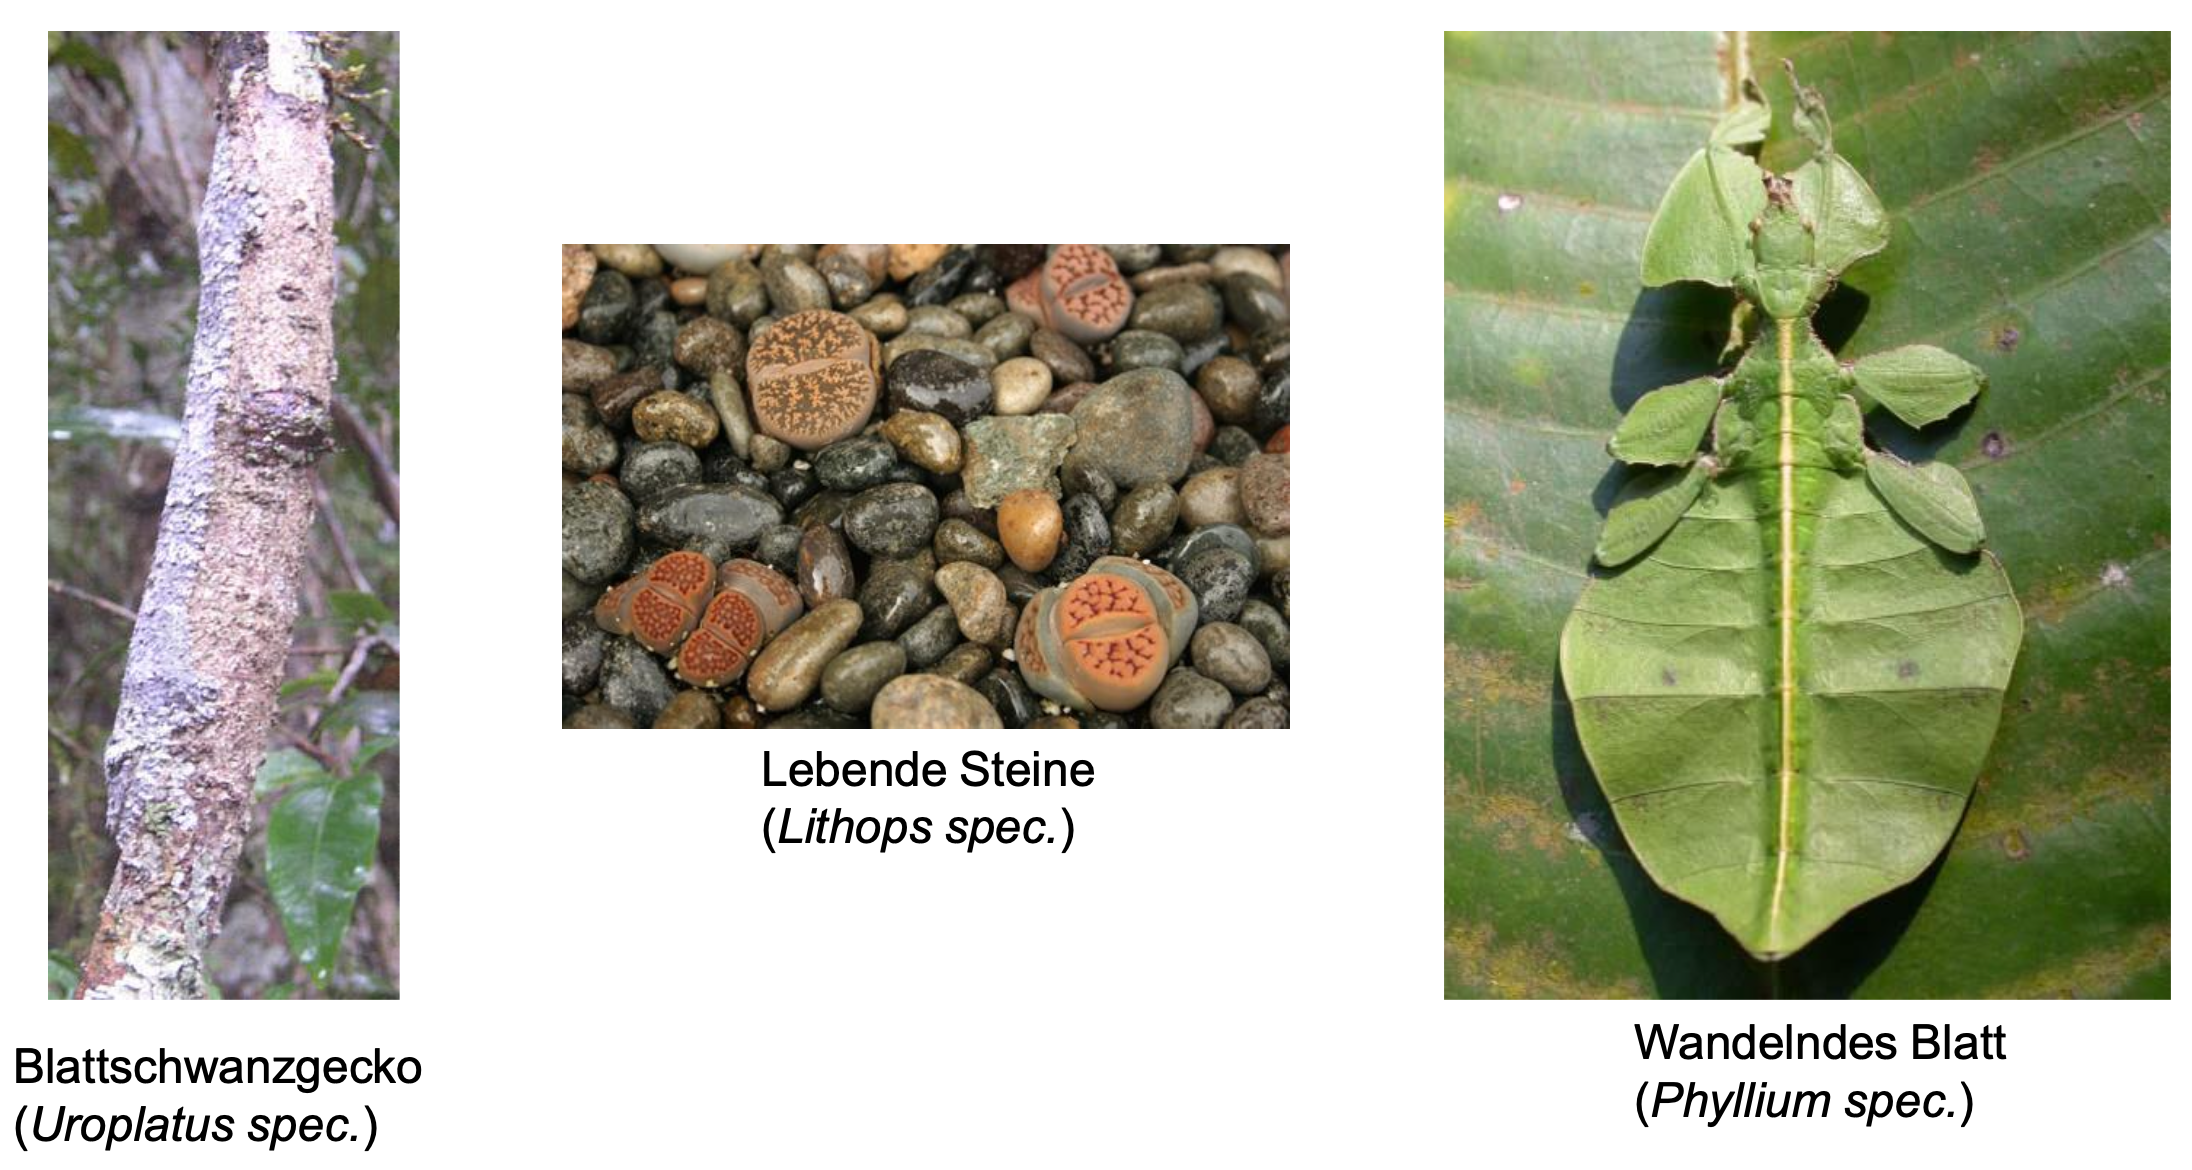
\includegraphics[width=8cm]{lec1/figures/Mimese.png}	
\end{center}
\textbf{Bates'sche Mimikry}: Ähnlichkeit von zwei Tierarten, wobei ein Tier ein ungenießbares Tier nachahmt.\\
\textbf{Mertens'sche Mimikry}: Ähnlichkeit von zwei Tierarten, wobei ein Tier ein giftiges Tier nachahmt. Dabei ahmen Tierarten vor allem mäßig giftige Tiere nach, da Angreifer nur bei diesen aus nicht-tödlichen Interaktionen lernen können.\\
\textbf{Peckham'sche Mimikry}: „Aggressive Mimikry“ die potentielle Beutetiere anlockt (z.B.\ Angel beim Seeteufel).

\subsection{Teilbereiche der Bionik}
Es werden folgende Beispiele genannt:
\begin{enumerate}
	\item \textbf{Leichtbau \& Materialien}: Selbstschärfende Messer für Industrieschneidemaschinen am Vorbild von Zähnen von Nagetieren. Dabei wird für die Spanfläche ein weiches Material und für die Freifläche ein hartes Material gewählt, sodass bei Abnutzung der Spanfläche die scharfe Schnittkante erhalten bleibt.
	\item \textbf{Oberflächen}: Selbstreinigende Oberflächen am Vorbild vom Lotus-Effekt and Blattoberflächen.
	\item \textbf{Fluiddynamik, Schwimmen \& Fliegen}: Der Kofferfisch hat einen geringen Strömungswiderstand (trotz seinen recht großen Körper). Diese Eigenschaft kann z.B. im Karosseriebau verwendet werden.
	\item \textbf{Biomechatronik \& Robotik}: Sechs- und mehrbeinige Tiere sind auch im Stand stabil (\textit{statisch stabile Gangart}). Vier- und zweibeinige Tiere sind dagegen nur bei Bewegung stabil (\textit{dynamisch stabile Gangart}).
	\item \textbf{Kommunikation \& Sensorik}: Das Infrarot-Organ des Schwarzen Kiefernprachkäfers kann als Vorbild für einen IR-Sensor verwendet werden.
	\item \textbf{Optimierung}: Die Struktur von Bäumen und Knochen kann zur Form- und Gewichtsoptimierung im Leichtbau verwendet werden ($\rightarrow$ Methode der Zugdreiecke nach dem Vorbild der gerundeten Ausformung von Astgabelungen).
	\item \textbf{Architektur \& Design}: Optimierung von Gebäudestrukturen (Leichtbau/ Ressourcenschonung/ hohe Stabilität).
\end{enumerate}

\subsection{Das Forschungsprinzip Bionik}

Biologen/ Grundlagenforscher verfolgen das bottom-up Prinzip \dangersign:
\begin{center}
	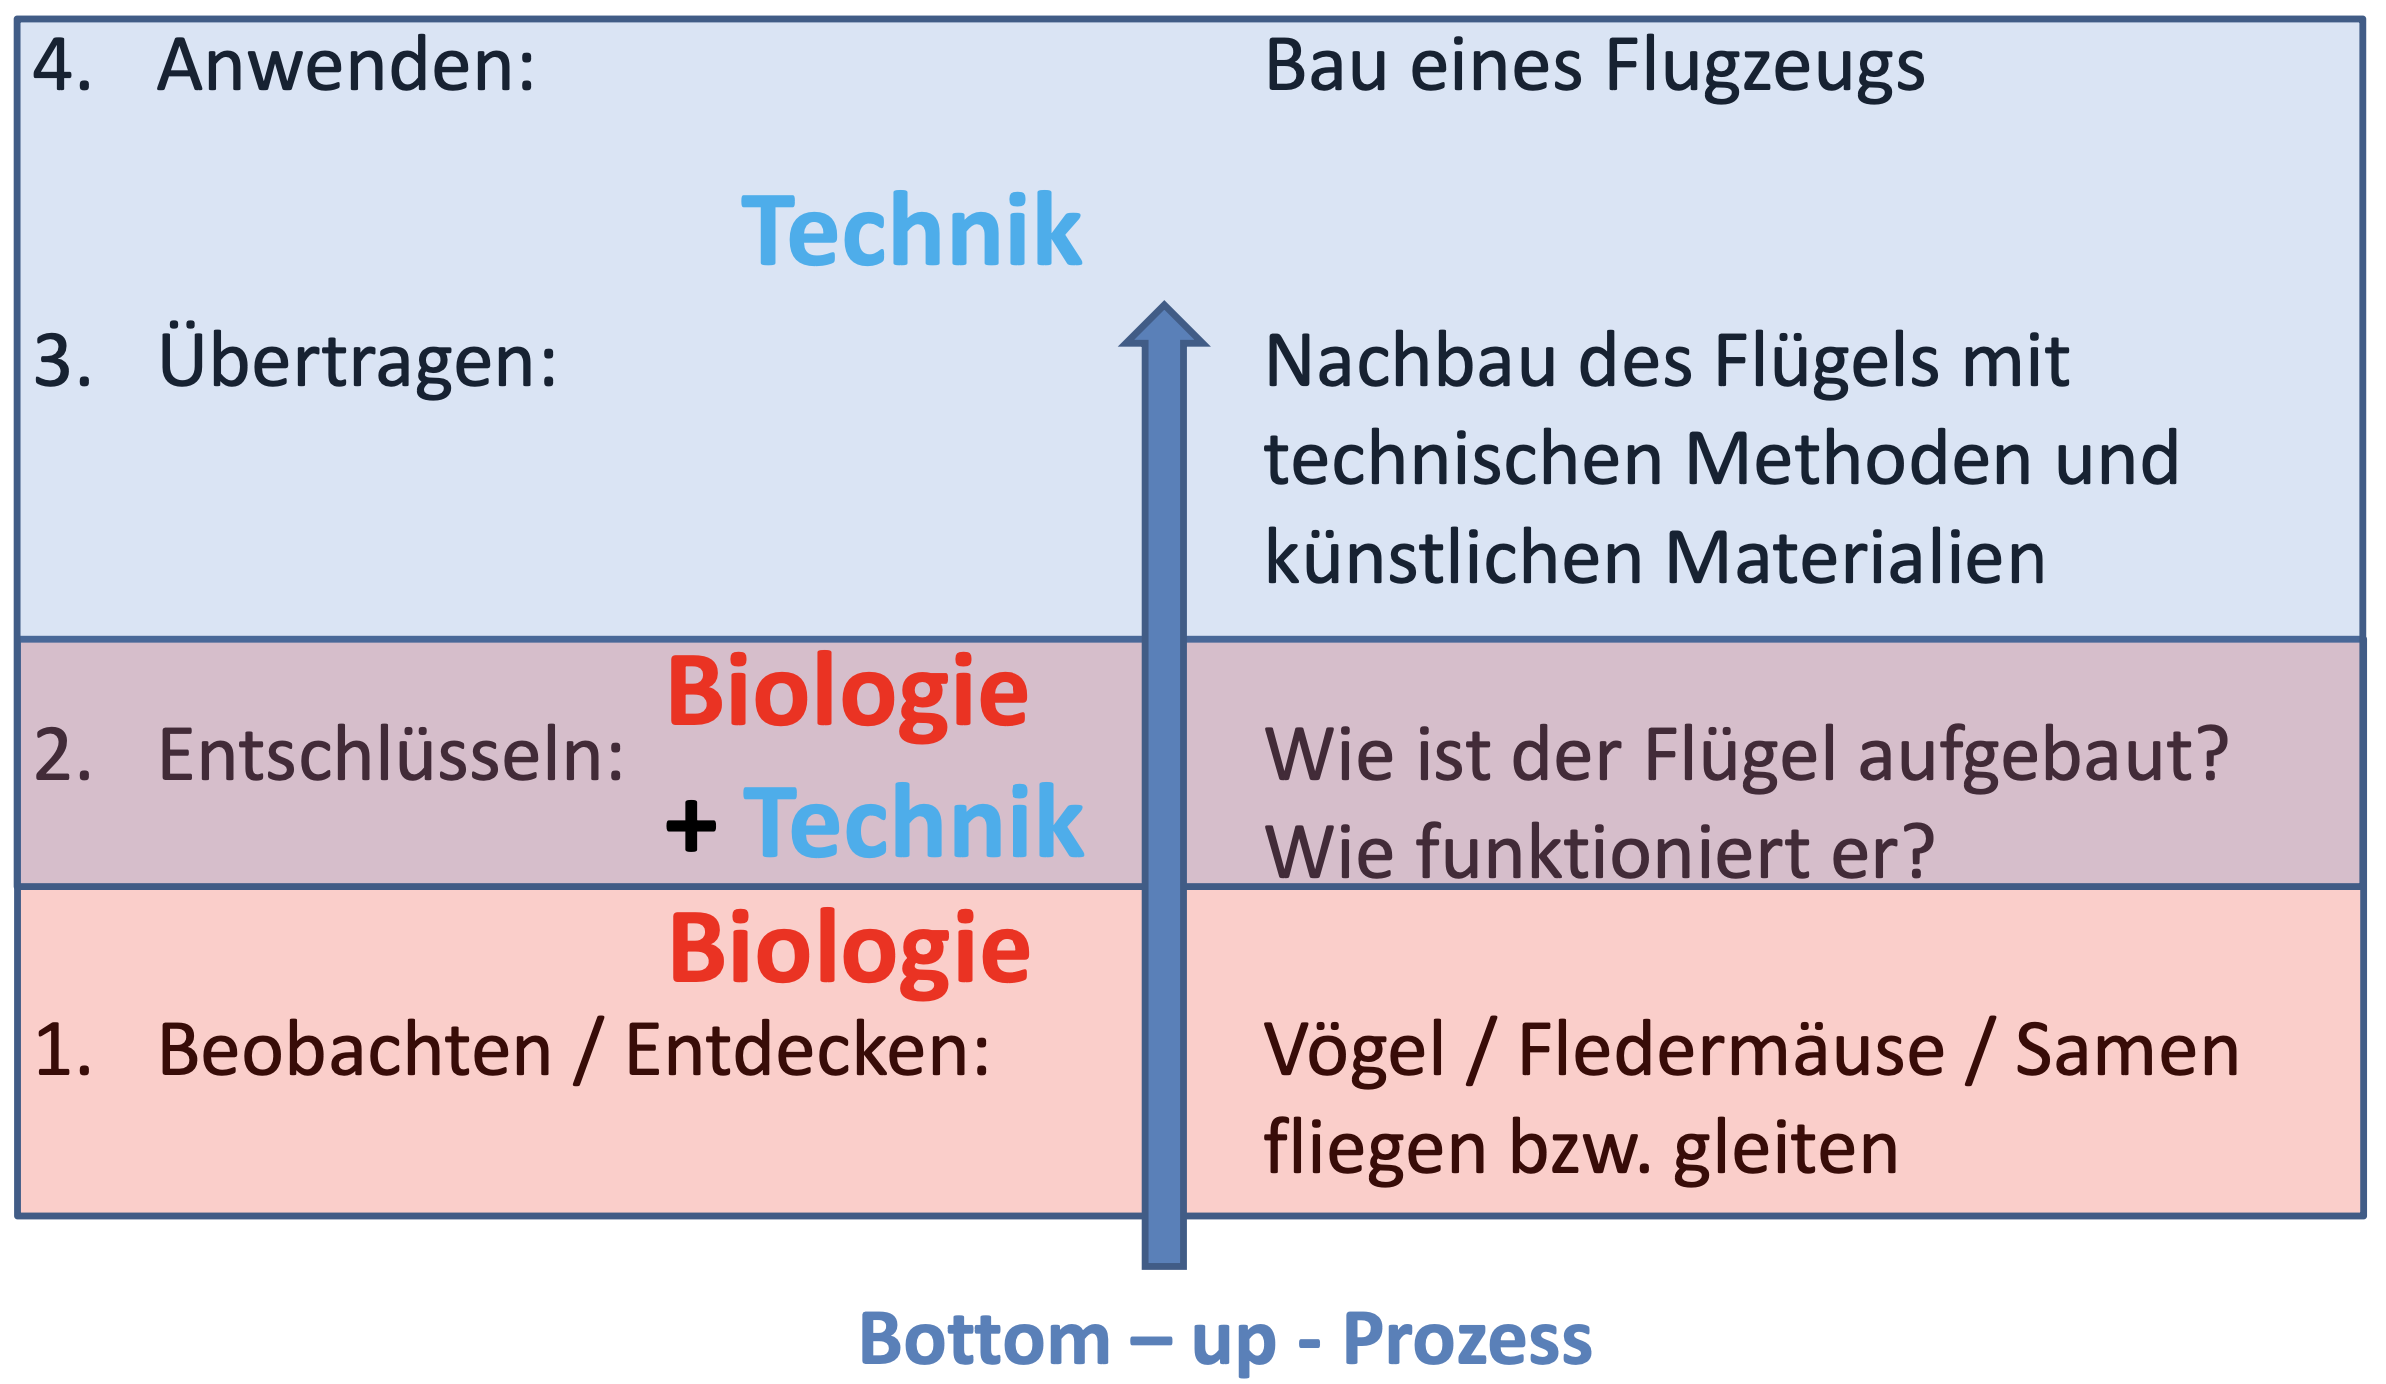
\includegraphics[width=10cm]{lec1/figures/Forschungsprinzip.png}	
\end{center}
Vorteile: Große Innovationshöhe. Nachteile: Erfolg/ Zeitbedarf sind nicht abschätzbar. ROI ist nicht gesichert $\rightarrow$ Bspl.\ Klettverschluss.\\
Der Ingenieur wird vom Optimierungsproblem her top-down getrieben (\dangersign \textit{Unterschiede zu bottom-up}):

\begin{center}
	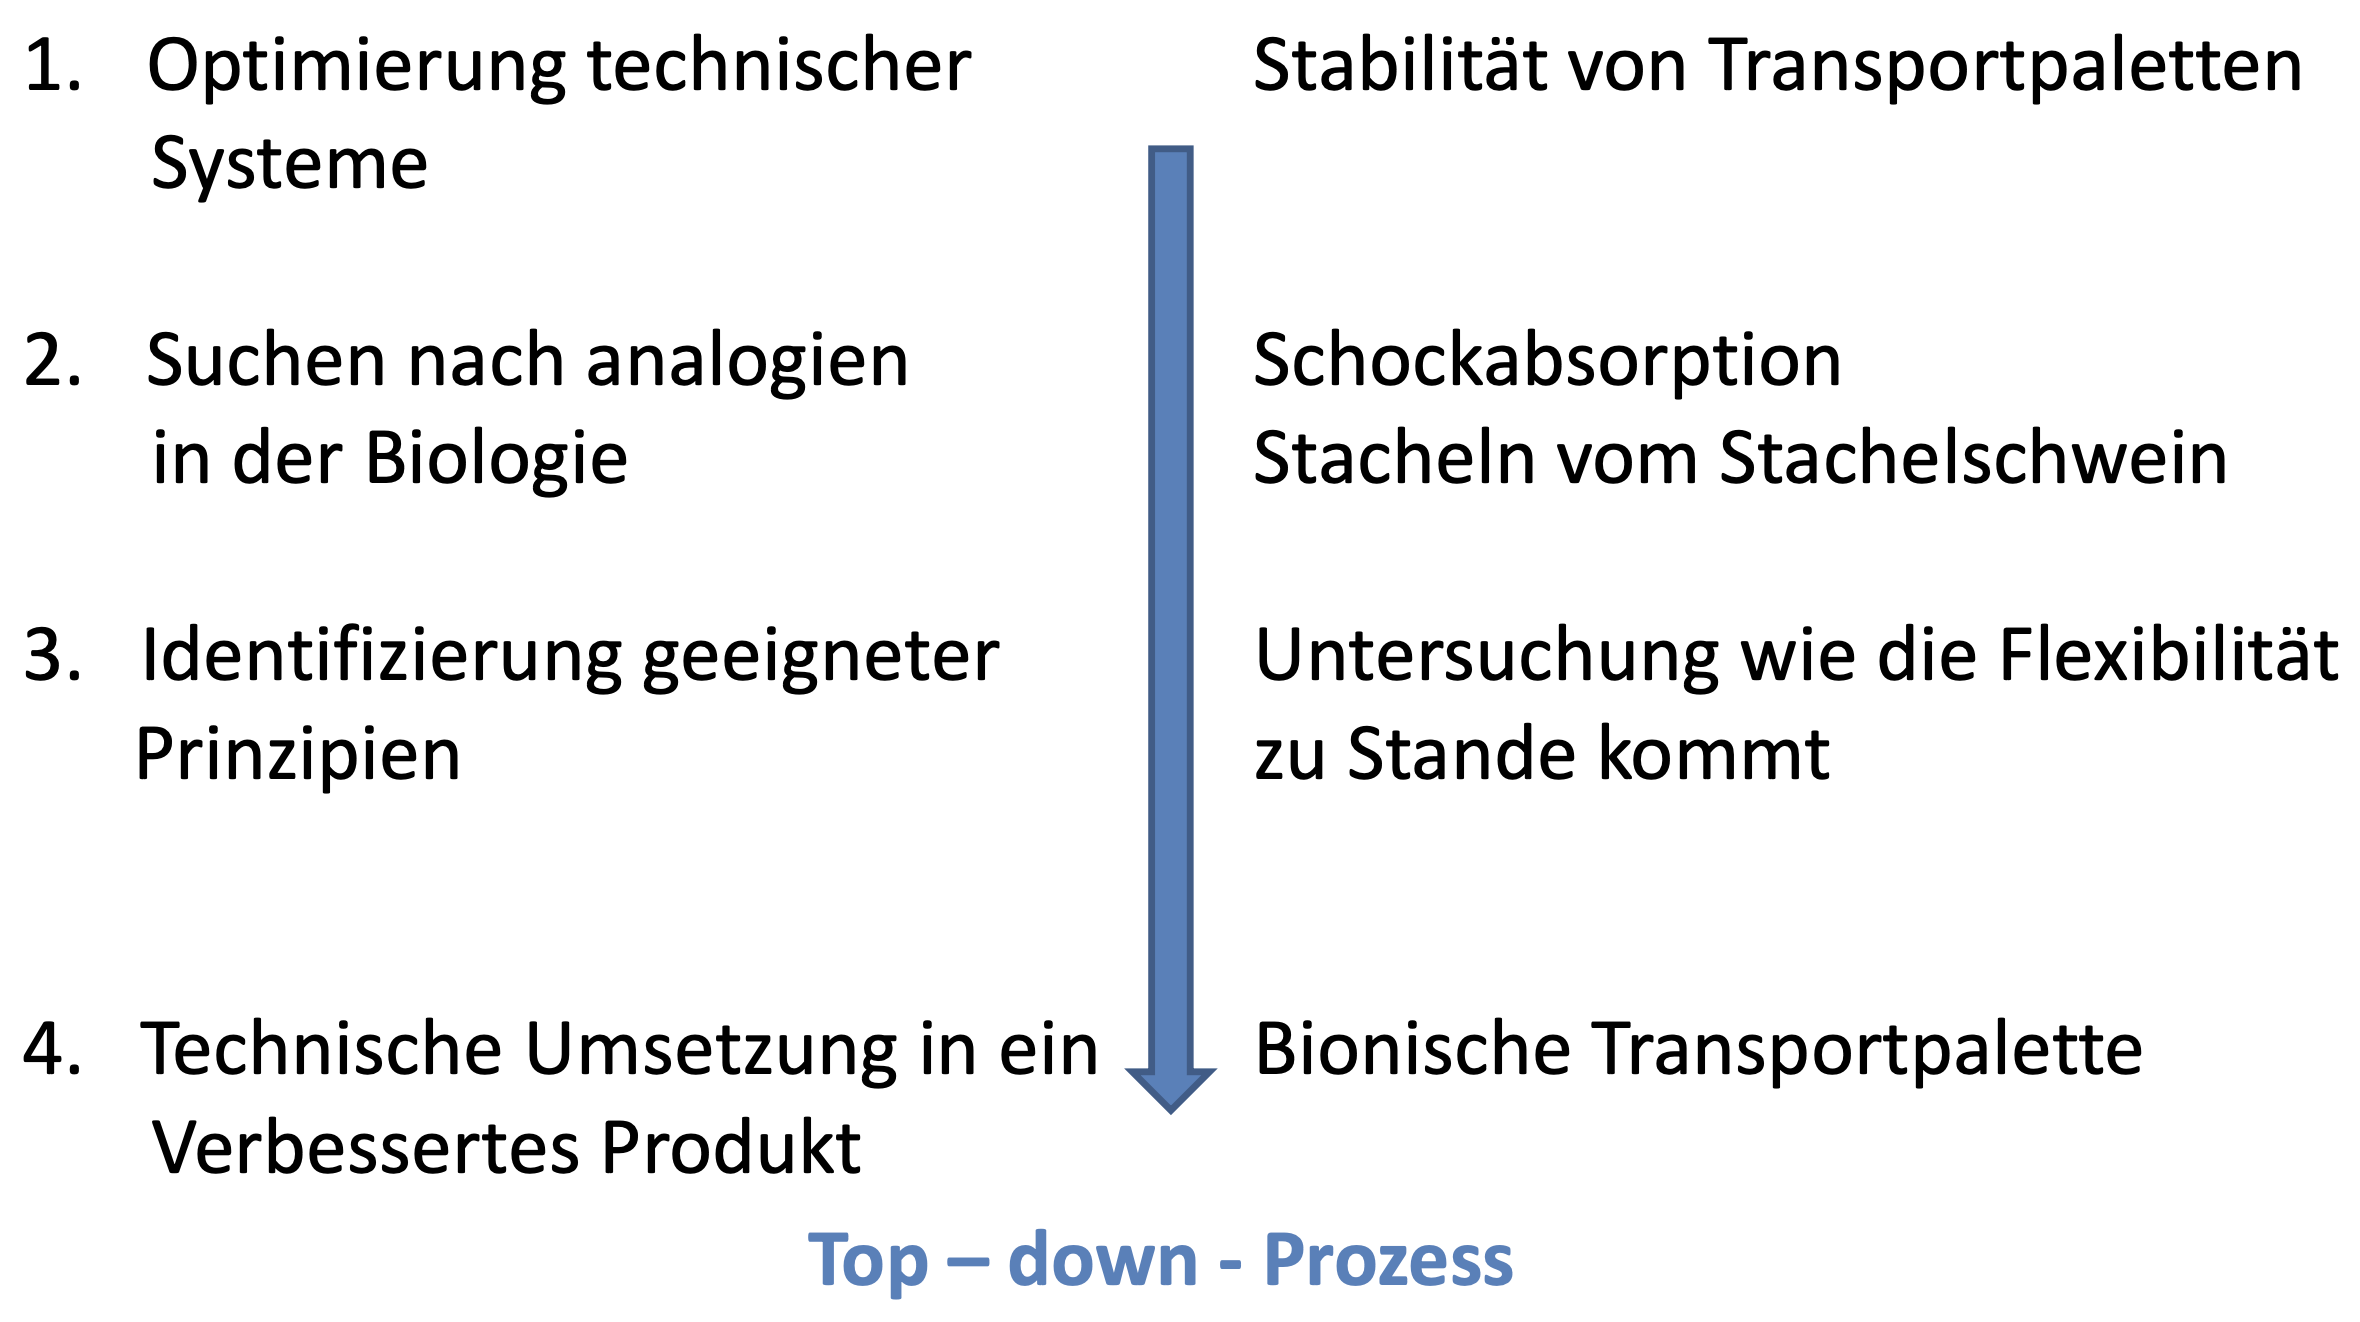
\includegraphics[width=10cm]{lec1/figures/top-down.png}
\end{center}
Vorteile: Erfolg/ Zeitbedarf sind abschätzbar. ROI ist gesichert. Nachteile: Geringe Innovationshöhe $\rightarrow$ Bspl.\ 
bionische Palette.\\
\\
Die Technische Biologie, Bionik und Reverse Bionik sind durch eine geschlossene Spirale verbunden:
\begin{center}
	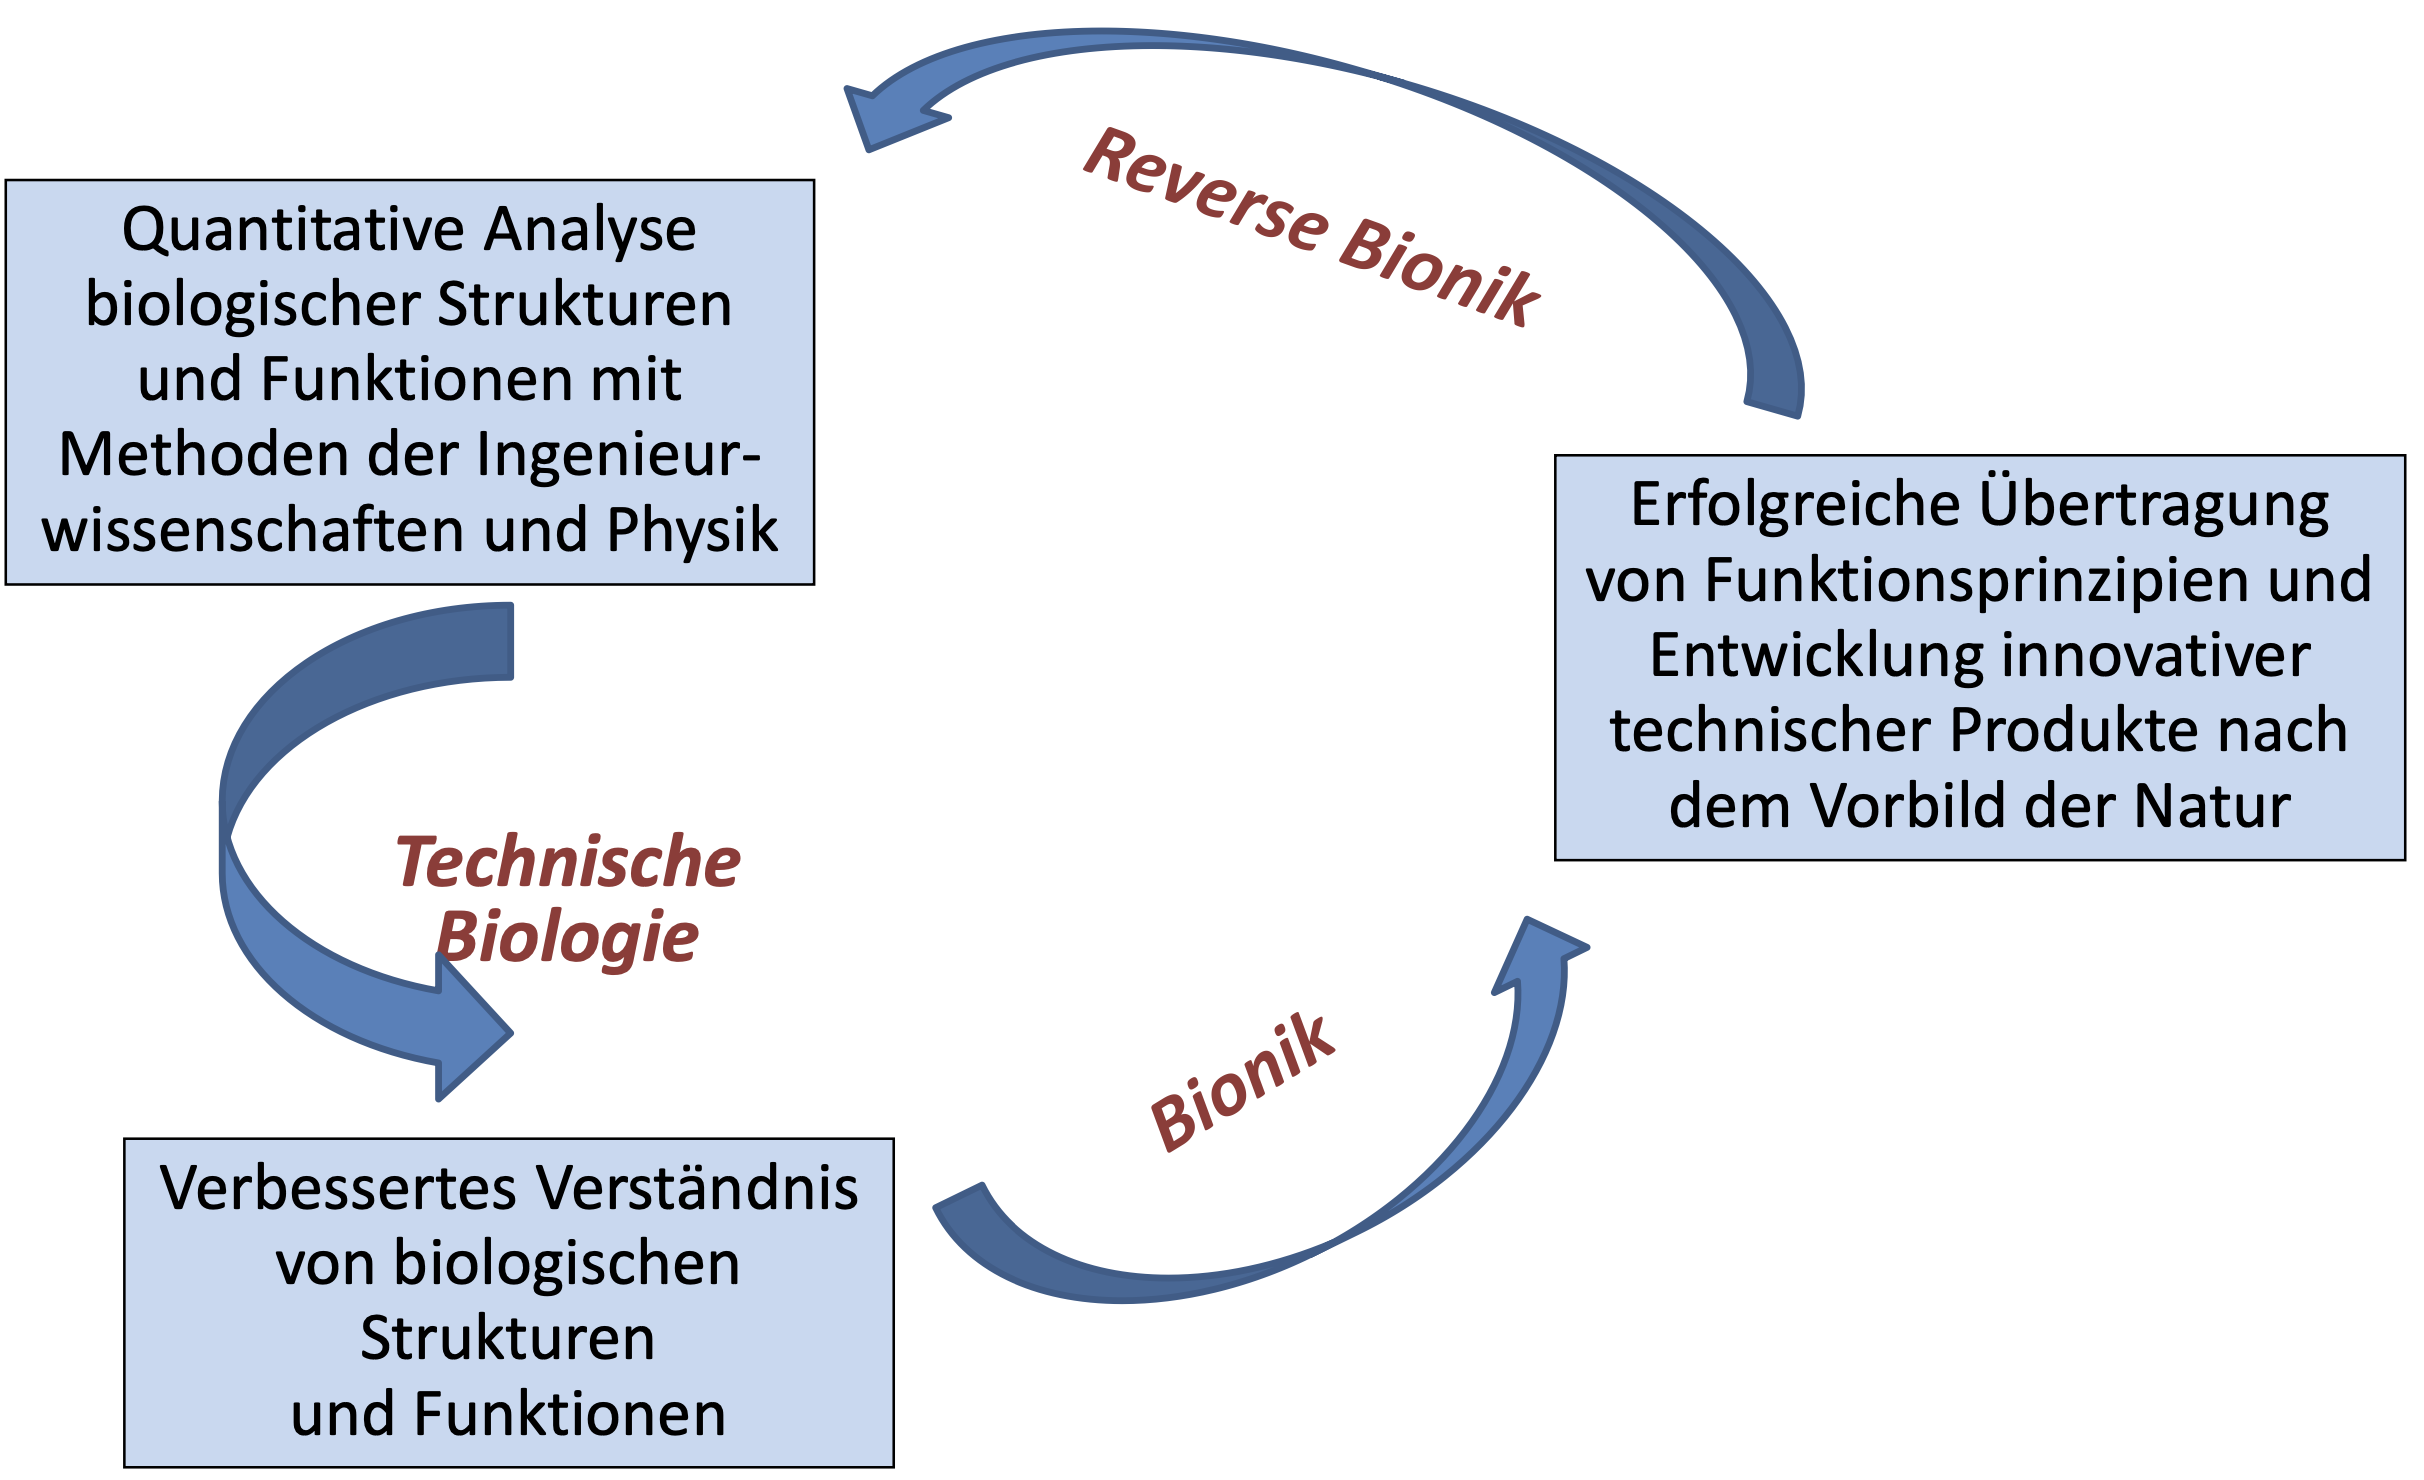
\includegraphics[width=10cm]{lec1/figures/spirale.png}
\end{center}

\subsection{Biologische Grundlagen}
Während bei der technischen Produktherstellung (Sägen, Stanzen, Schneiden, etc.) das Endprodukt aus einem Werkstückrohling i.d.R.\ durch Abtragung von Material geschieht, entstehen biologische Produkte durch \textit{genetische kontrollierte Selbstorganisation} (Molekül $\rightarrow$ Organell $\rightarrow$ Zelle $\rightarrow$ Gewebe $\rightarrow$ Organ $\rightarrow$ Spezies) -- \textcolor{red}{Komplexitätszunahme durch hierarchisches Wachsen} \dangersign. 3D-Drucker imitieren hier eher die biologische Produktherstellung.
\\
\\
Was ist eine \textbf{Spezies}? Nach dem \textbf{Morphologischen Artkonzept} geschieht die Unterscheidung anhand von morphologischen (äußeren) Merkmalen. Das \textbf{Ethologischen Artkonzept} trifft die Unterscheidung anhand des Verhaltens. Beim \textbf{Populationsgentischen Artkonzept} ist das entscheidende Merkmal, ob sich Populationen zweier Arten miteinander fortpflanzen können und fertile Nachkommen zeugen (``Biospezies''). Geographische/ ökologische Isolation zweier Populationen kann langfristig auch zur reproduktiven Isolation führen. 

Nachkommen zweier Spezies werden \textit{Allospezies} genannt, wenn sie fertil sind, und \textit{Hybride} wenn nicht. Es gibt allerdings auch Spezies, die sich nicht mit dem Populationsgenetischen Artkonzept abgrenzen lassen (z.B. Bakterien).
\\
\\
Der Census of marine life schätzt die \textbf{Artenvielfalt} auf ca.\ 8,7 Mio.\ Spezies, wovon lediglich 1,2 Mio. beschrieben sind (60\% davon Insekten). Die biologischen Hot-Spots sind der tropische Regenwald:

\begin{center}
	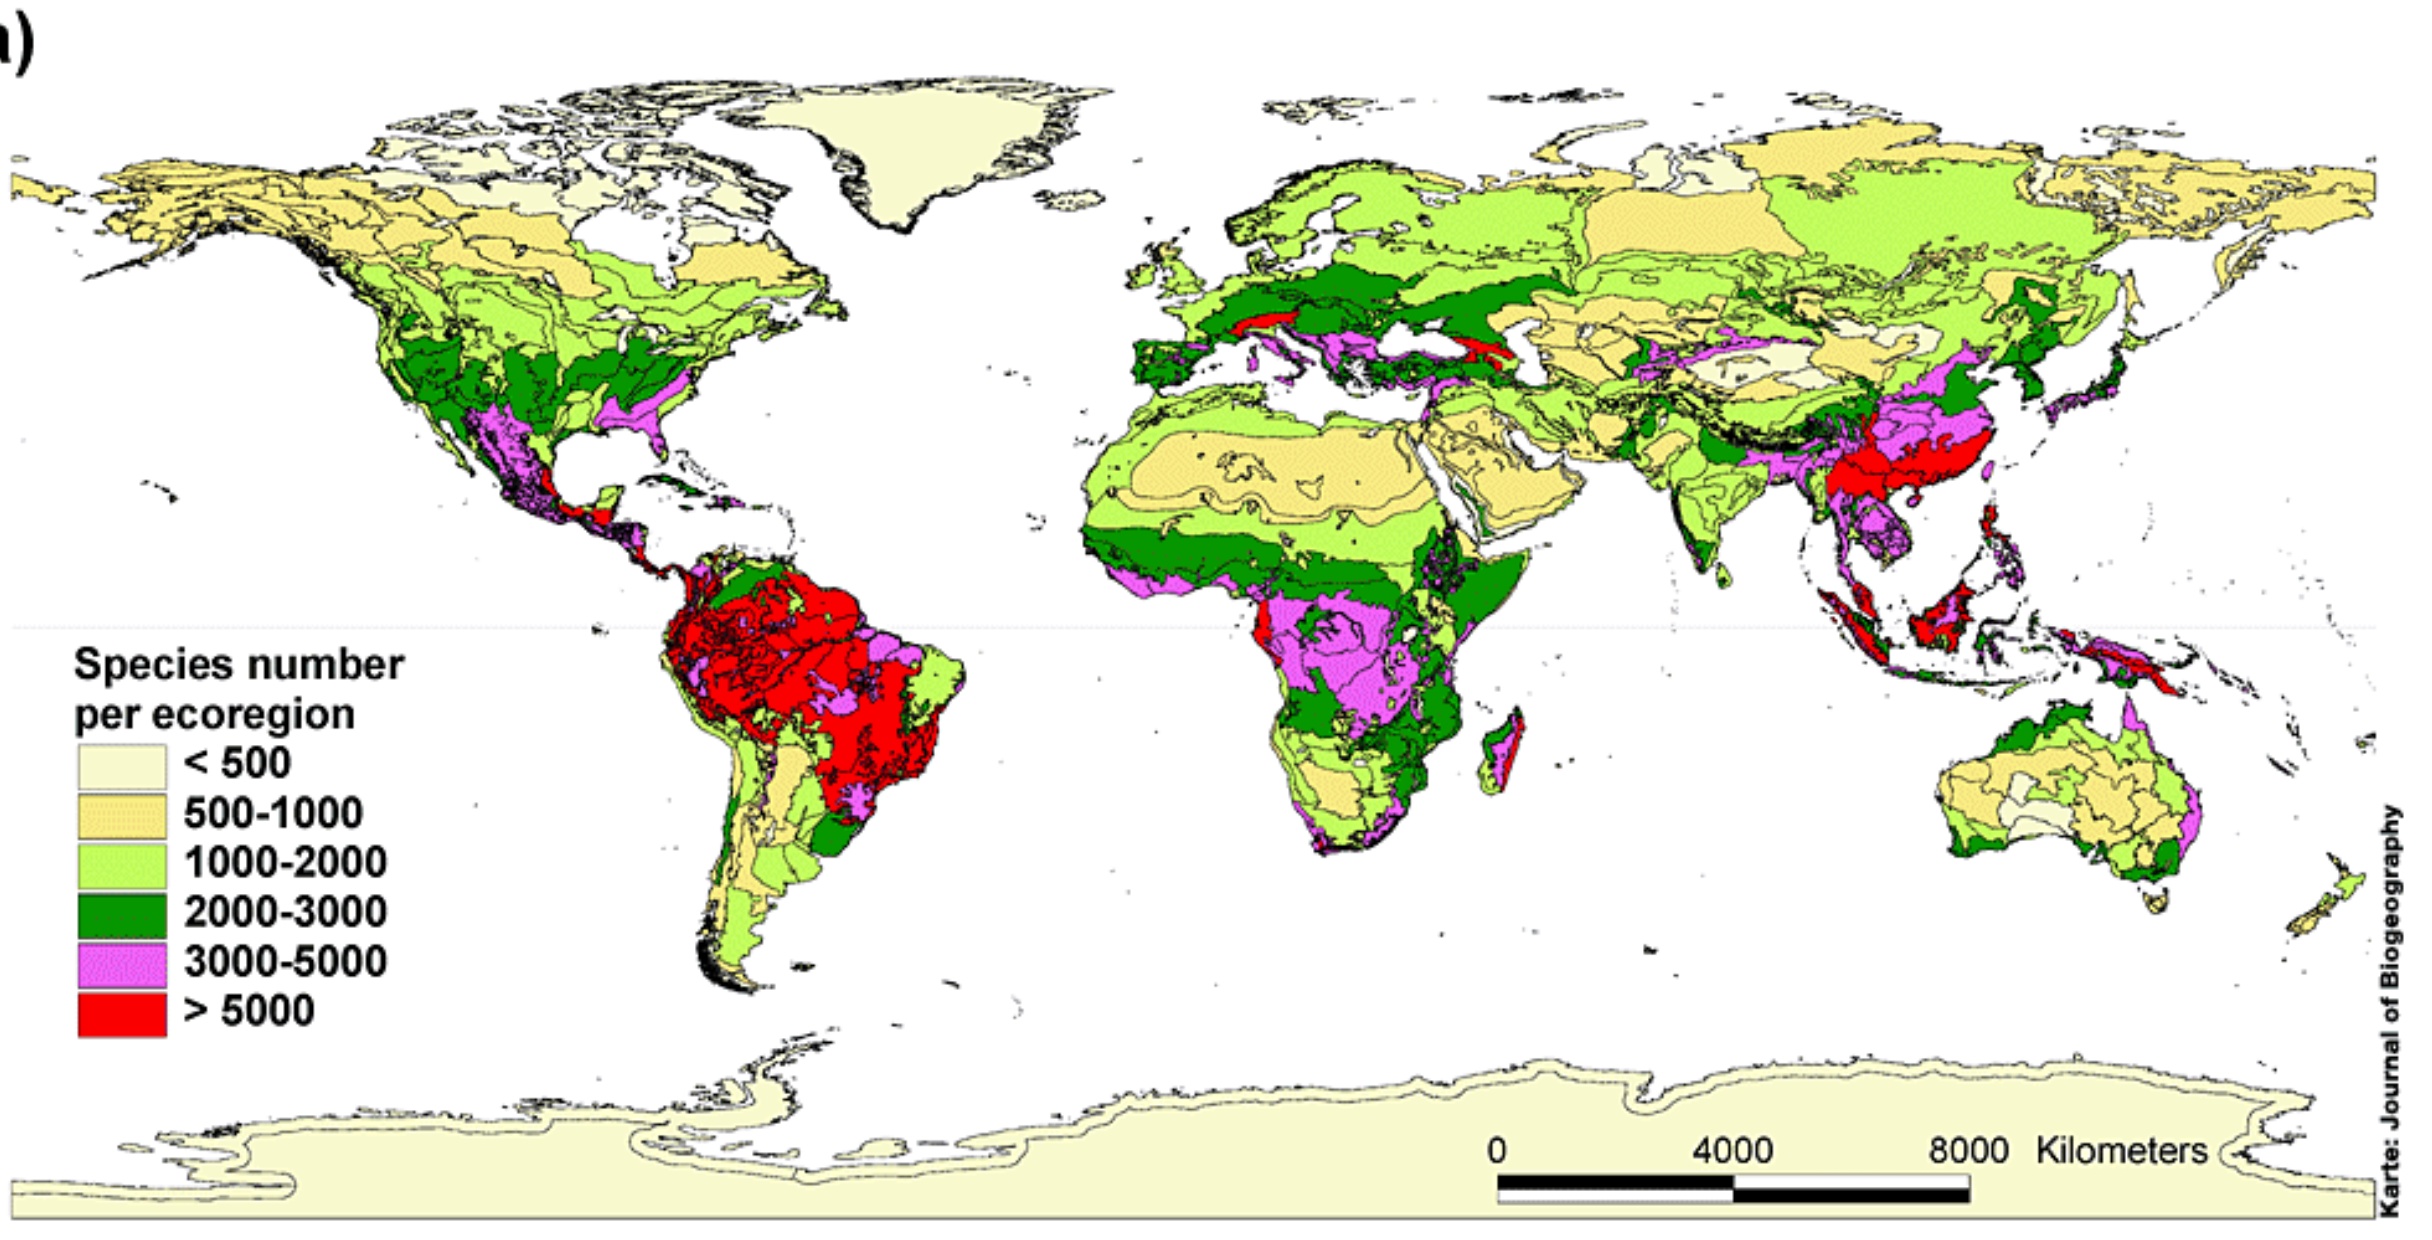
\includegraphics[width=10cm]{lec1/figures/bio-hotspots.png}
\end{center} 
Gerade diese Gebiete sind allerdings auch von Waldbränden, Abholzung und dem Klimawandel besonders bedroht. Dies ist ein Problem für die Bionik, denn jede ausgestorbene Art könnte eine bionische Lösung darstellen \dangersign.

\subsubsection{Systematik der Arten}

Klassischerweise erfolgt die Bestimmung und Benennung von Arten nach der Systematik: Gattungsname, Artenname, Unterart (weitere veraltete Einteilungen). Heute folgt man der \textbf{Phylogenetische Systematik}, wobei die Verwandschaftsbeziehung zwischen den Arten dargestellt wird. Dabei entstammen jeder Verzweigung immer zwei Äste und jeder Ast wird durch ein abgeleitetes Merkmal begründet.

\begin{center}
		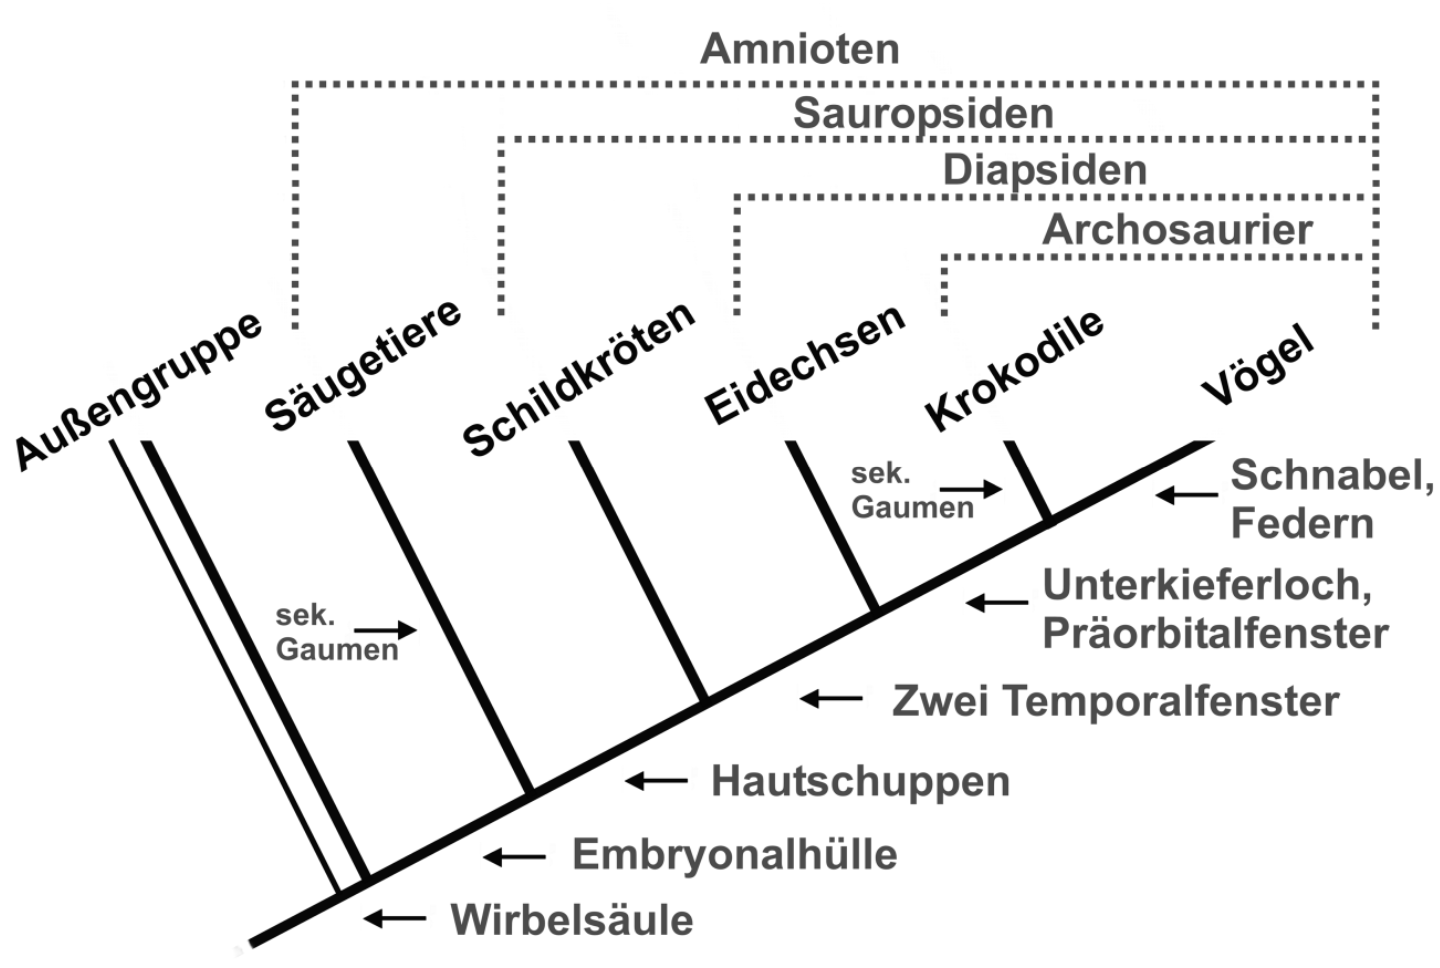
\includegraphics[width=9cm]{lec1/figures/phylogenetische_systematik.png}
\end{center}
\begin{center}
	\begin{itemize}
		\item \textbf{Apomorphie}: Merkmal welches im Vergleich zum direkten Vorfahren neu erworben wurde („abgeleitetes Merkmal“) $\rightarrow$ beim Vogel: Schnabel, Federn.
		\item \textbf{Plesiomorphie}: Gegenbegriff zur Apomorphie. Merkmal, welches bereits vor der Abstammungslinie entstanden ist („ursprüngliches Merkmal“) $\rightarrow$ beim Vogel: z.B. Wirbelsäule. (\dangersign \textit{Unterschied: plesiomorphe/apomorphe Merkmale})
		\item \textbf{Schwestergruppen}: Aufspaltung einer Stammart in zwei Gruppen aus einem gemeinsamen unmittelbaren Vorfahren. $\rightarrow$ z.B. Krokodile und Vögel
		\item \textbf{Synapomorphie}: Gemeinsamer Besitz eines apomorphen Merkmals $\rightarrow$ z.B. Unterkieferloch, Präorbitalfenster bei Krokodilen und Vögeln
		\item \textbf{Monophyletische Gruppe}: Systematische Einheit, die den gemeinsamen Vorfahren und alle seine Nachfahren enthält. $\rightarrow$ z.B. Krokodile, Vögel
		\item \textbf{Paraphyletische Gruppe}: Systematische Gruppe, die den gemeinsamen Vorfahren aber nicht alle Nachfahren enthält. $\rightarrow$ z.B. Schildkröten, Eidechsen und Krokodile (Vögel fehlen)
		\item \textbf{Analogie}: Durch \textit{konvergente Entwicklung} entstandene Merkmale, die unabhängig voneinander entstanden sind. Erfüllen die gleiche Aufgabe sind aber nicht auf einen gemeinsamen Vorfahren zurückzuführen. $\rightarrow$ sek. Gaumen bei Säugetieren und Krokodilen. (Diese Eigenschaften sind in der Bionik besonders interessant)
	\end{itemize}
\end{center}
\textbf{Konvergente Entwicklung \dangersign:} Wenn sich bei zwei Spezies ähnliche Funktionsprinzipien entwickeln, die aber nicht auf einen gemeinsamen Vorfahren zurückzuführen sind. Bspl.\ Grabschaufeln der Maulwurfsgrille und Maulwurf.

\begin{center}
    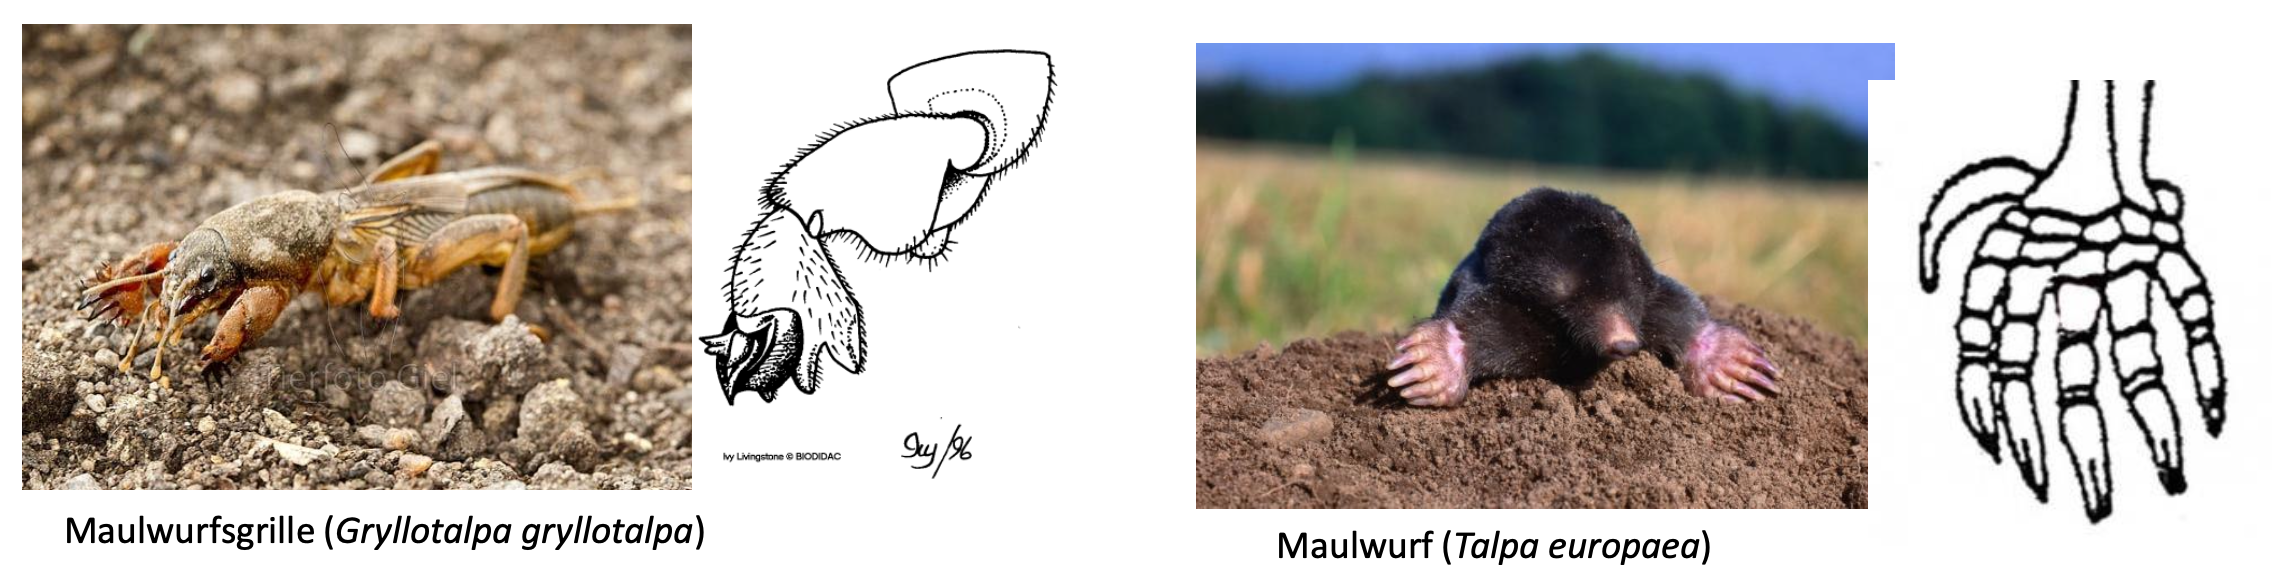
\includegraphics[width=10cm]{lec1/figures/maulwurf.png}    
\end{center}

\subsubsection{Entstehung von Merkmalen}

\textbf{Lamarckismus \dangersign:} Organismen vererben Eigenschaften an ihre Nachkommen, die sie während ihres Lebens erworben haben.
\\
\textbf{Darwinismus:} Die Organismen, welche am besten an ihre Umgebung angepasst sind, werden durch die natürliche Selektion begünstigt und vererben Eigenschaften an ihre Nachkommen. 

Bei der Vererbung kann neben der Weitergabe der Merkmale and Nachkommen, genetische Variabilität durch Mutationen der DNA entstehen.
Die Variabilität der Individuen führt zu unterschiedlichen
Überlebensraten und Fortpflanzungserfolg und damit zur \textbf{natürlichen Selektion}. Individuen mit Merkmalen, die zu einer bessere Anpassung an die Umwelt führen treten in der nächsten Generation vermehrt auf.
\\
\\
\textbf{Selektionsfaktoren} (Umweltfaktoren mit Einfluss auf die ``Fitness'' eines Individuums):
\begin{itemize}
	\item Abiotisch: Licht, Temperatur, Drucke, Feuchtigkeit, Wind
	\item Biotisch: Zwischenartlich und innerartlich
	\item Künstlich: Zucht durch Menschen
\end{itemize}
\textbf{Sexuelle Selektion}: Auslese von Individuen durch Vorteile beim Fortpflanzungserfolg gegenüber Geschlechtsgenossen derselben Art.
\\\\
\textbf{Was ist eine Ringspezies \dangersign?} Eine Ringspezies besteht aus mehreren meist morphologisch deutlich unterscheidbaren Populationen (welche unter Umständen formal als eigenständige Arten klassifiziert werden), bei denen Individuen benachbarter Populationen sich kreuzen und Gene austauschen können, dies jedoch zumindest bei einigen der nicht-benachbarten Populationen nicht mehr möglich ist (siehe Wikipedia). Bspl: Salamander der Gattung Ensatina.

\subsection{Fehleinschätzungen \& Grenzen der Bionik}

3 Fehleinschätzungen:
\begin{enumerate}
	\item Bionik liefert optimale Lösungen. (``optimiert ist nicht optimal'')
	\item Bionik ist ressourcenschonend und umweltfreundlich
	\item Bionik besteht vor allem aus Übertragung von Technik (ist vor allem Grundlagenforschung)
\end{enumerate}
Grenzen \dangersign: Die Evolution hat keine Richtung und ist ein dynamischer Prozess. D.h.\ \textcolor{red}{Merkmale werden nur soweit wie nötig optimiert und es können alternative Entwicklungsformen entstehen, wenn diese optimaler als Hochleistungsmerkmale sind}. Wie z.B. bei der Kerguelen-Fliege, die in einer stark windigen Umgebung ihre Flügel zurückgebildet hat (und nun am Boden lebt), anstatt stärkere zu entwickeln. 
\begin{center}
	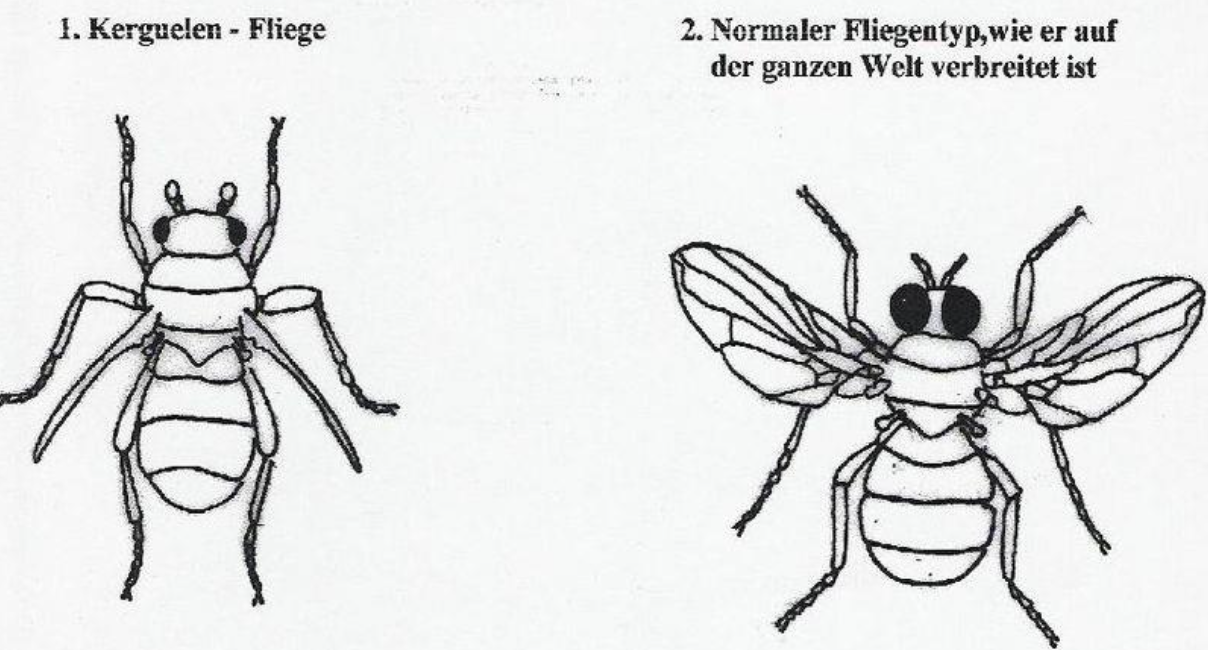
\includegraphics[width=6cm]{lec1/figures/fliege.png}
\end{center}

\section{Superhydrophobe Oberflächen}

\textbf{Was sind \glqq smart materials\grqq \dangersign?} Festkörper, Flüssigkeiten oder Gase, die selbständig auf veränderte Umwelteinflüsse reagieren (können). Ein Beispiel für ein \glqq smart material\grqq\ ist die \textbf{Cuticula}, die Grenzfläche zwischen Pflanze und Umwelt. Diese wird auch als äußere Epidermiszellwand bezeichnet. Die Cuticula findet sich in der Wachsschicht von Trauben, Lotus-Blättern und Stacheln von Kakteen. 

\subsection{Plfanzenkutikula - Funktionen und Struktur}

\begin{center}
	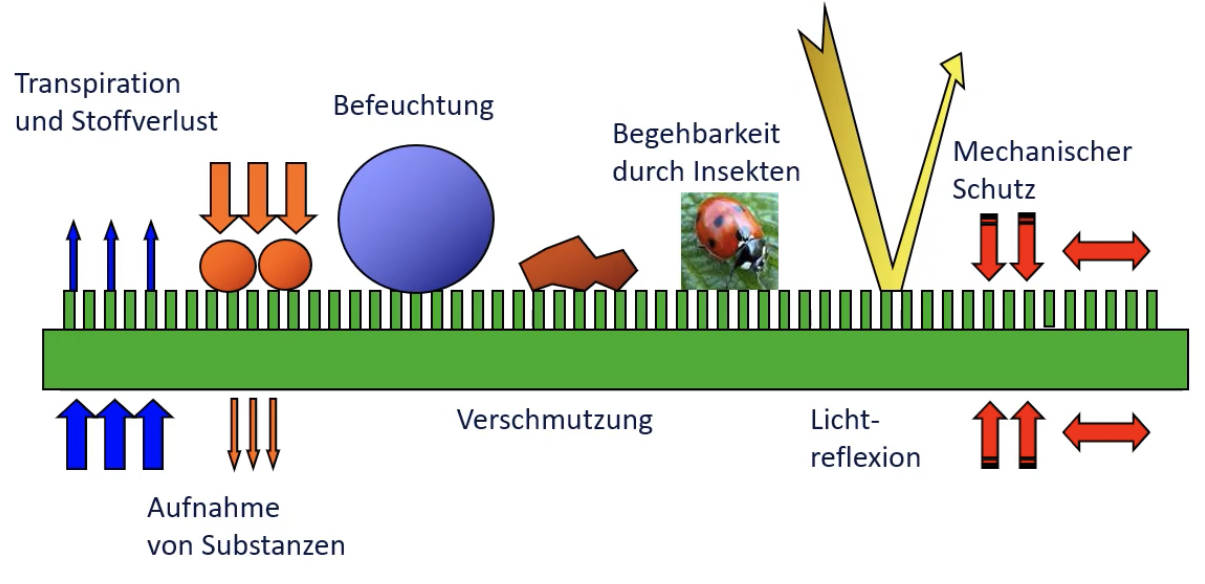
\includegraphics[width=10cm]{lec2/figures/kutikula-funktionen.png}
\end{center}
(\dangersign \textit{Nenne vier Funktionen der Pflanzenkutikula.})

\begin{itemize}
    \item Transpiration und Stoffverlust
    \item Aufnahme von Substanzen
    \item Befeuchtung
    \item (Vermeidung von) Verschmutzung
    \item Begehbarkeit durch Insekten (z.B.\ um Schädlinge zu konsumieren)
    \item Lichtreflexion (z.B.\ in Wüstenregionen bei zu starker UV-Strahlung)
    \item Mechanischer Schutz
\end{itemize}
Das Blatt besteht aus verschiedenen Zelltypen, wie in dem folgenden Querschnitt zu sehen ist. Während die Cuticula und Epidermis schützen und die Interaktion mit der Außenwelt kontrollieren, bilden die oberen Zellen eine Stützstruktur und die unteren Zellen ein Leitsystem für Wasser und Nährstoffe.
\\\\
\textit{Anmerkung: Die Komponenten des hier abgebildeten Blattquerschnitts müssen nicht auswendig gelernt werden}.

\begin{center}
	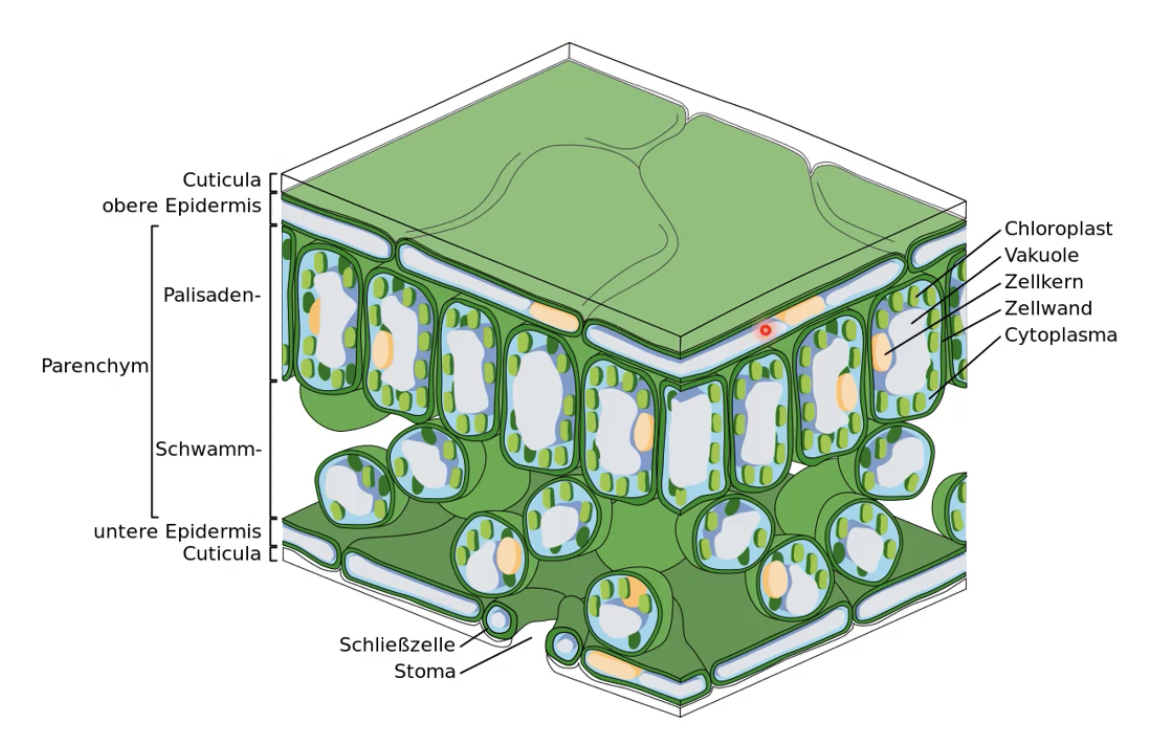
\includegraphics[width=8cm]{lec2/figures/blatt-querschnitt.png}	
\end{center}
Der \textbf{strukturelle Aufbau der Kutikula} ist idealisiert ein schichtweißer Aufbau. In der Realität handelt es sich allerdings um Verbundmaterialien, welche technisch aufwändig zu rekonstruieren sind. Die einzelnen Schichten bestehen dabei aus verschiedenen Alkoholen und Fettsäuren.

\begin{center}
	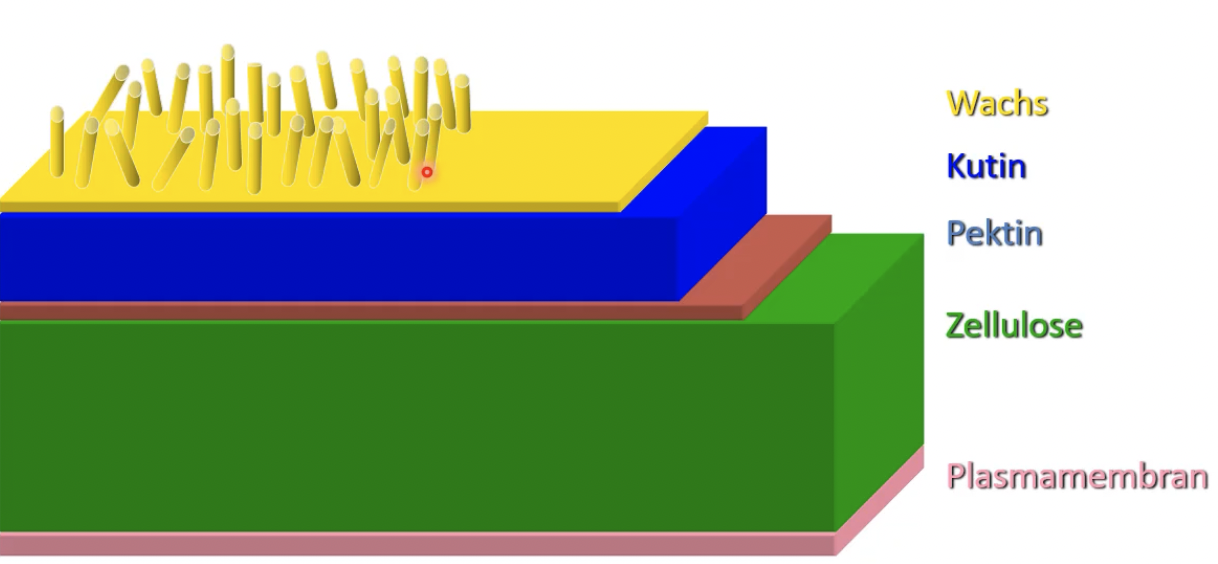
\includegraphics[width=8cm]{lec2/figures/kutikula-aufbau.png}	
\end{center}

\subsection{Messmethoden für Oberflächen}

\subsubsection{Raster-Elektronen-Mikroskop (REM)}

Das REM rastert die Obefläche der Probe mit einem sehr feinen Elektronenstrahl ab. Die Elektronen werden aus einer Elektronenquelle gewonnen, über Spulen fokussiert, beschleunigt und treffen auf die Probe auf. Die dort ausgelössten Effekte (z. B. Strahlungseffekte) werden von verschiedenen Dektoren erfasst und geben rückschlisse auf \textbf{Topografie, Materialkontrast und Zusammensetzung} der Probe. Die Rohbilder sind immer in schwarz-weiß, können aber in der Nachbearbeitung anhand der Graustufen eingefärbt werden.\\

\begin{center}
	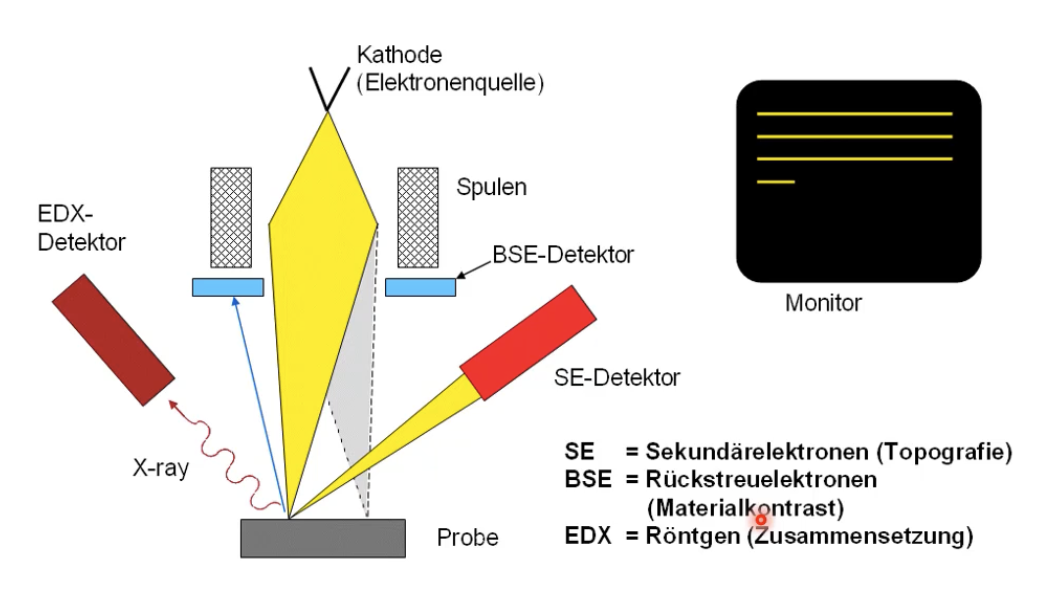
\includegraphics[width=8cm]{lec2/figures/rem.png}	
\end{center}
Um im Rahmen der bionischen Entwicklung geeignete Strukturen und Materialien zu finden, werden zunächste REM Aufnahmen verschiedener Oberflächen untersucht. Bei Pflanzen gibt es z.B.\ glatte Oberflächen, Pallisadenstrukturen und Wellenformen. Die Ausprägung der Kutikula liefert allerdings noch nicht genug Informationen darüber, ob ein gewisser Effekt durch sie bedingt ist. Daher sollten im Rahmen der bionischen Untersuchung im Stammbaum getrennte Arten mit ähnlichen Strukturen auf einen gewünschten Effekt hin getestet werden. Tritt dieser auf, so liegt die Vermutung nahe, dass die Oberfläche dafür verantwortlich ist.
\\\\
Pflanzliche Oberflächen sind oftmals rauh und haben diverse Strukturierungsmöglichkeiten mit Spalten, Fäden und Papillen (Zapfen). Auch das Wachs kann sich sehr unterschiedlich ausbilden und bietet eine Auswahl an Mikrostrukturen.

\subsubsection{Weißlicht-Profilometrie (WP)}

Bei der WP wird eine Quantifizierung der Topographie erzielt (Höhenmessung). Dafür werden Interferenzmuster ausgenutzt, um die Höhe von Mikrostrukturen auf der Oberfläche im $\mu$-meter Bereich zu messen.

\begin{center}
	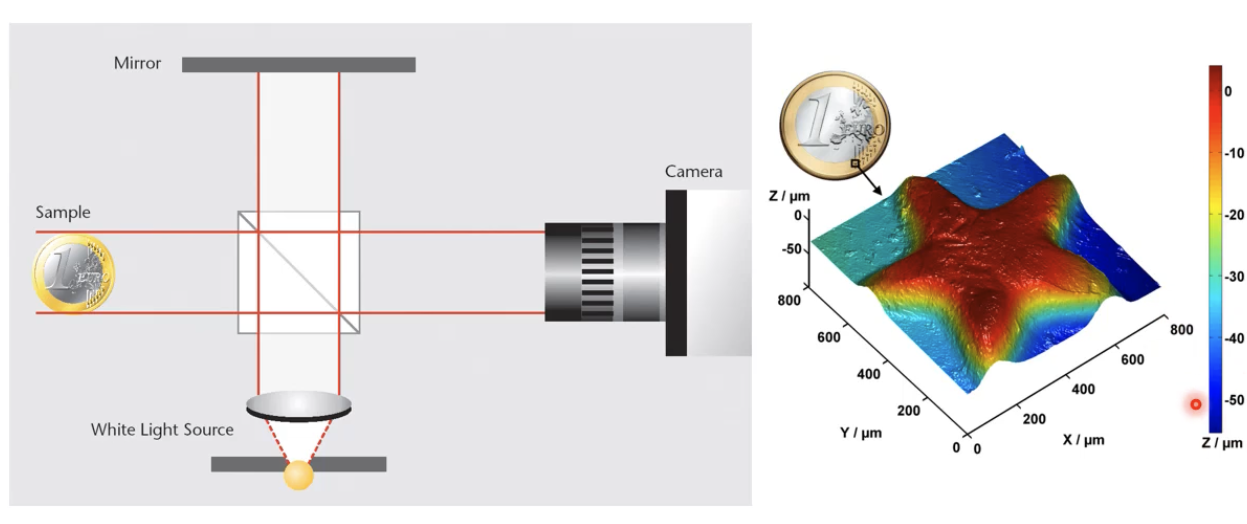
\includegraphics[width=8cm]{lec2/figures/wp.png}	
\end{center}

\subsection{Antiadhesion}

Bei wasserabweisenden Plfanzen tritt der Effekt der \textbf{Antiadhesion} auf. Die Blätter sind unbenetzbar und das Wasser perlt in Tropfen ab. Bekanntester Vertreter ist die Lotus-Pflanze. Der Effekt wurde im Rahmen der Reinigung entdeckt, welche notwendig ist, um REM-Aufnahmen der Oberfläche zu erstellen. Verantwortlich dafür ist eine hohe Rauheit und eine Papillenartige Mikrostruktur.

\subsubsection{Maße zur Beschreibung der Antiadhesion/ Benetzung}

\textbf{Rand-/ Kontaktwinkel $\Theta$} (\dangersign \textit{fertige eine Skizze an)}\\
Der Rand-/ Kontaktwinkel $\Theta$ liefert ein \textcolor{red}{Maß für die Benetzungsfähigkeit einer Oberfläche} mit $\Theta \in [1^\circ,179^\circ]$. Die \textbf{Young'sche Gleichung} zur Bestimmung von $\Theta$ beschreibt dabei das Vernetzungsverhalten zwischen drei Phasen.

\begin{center}
	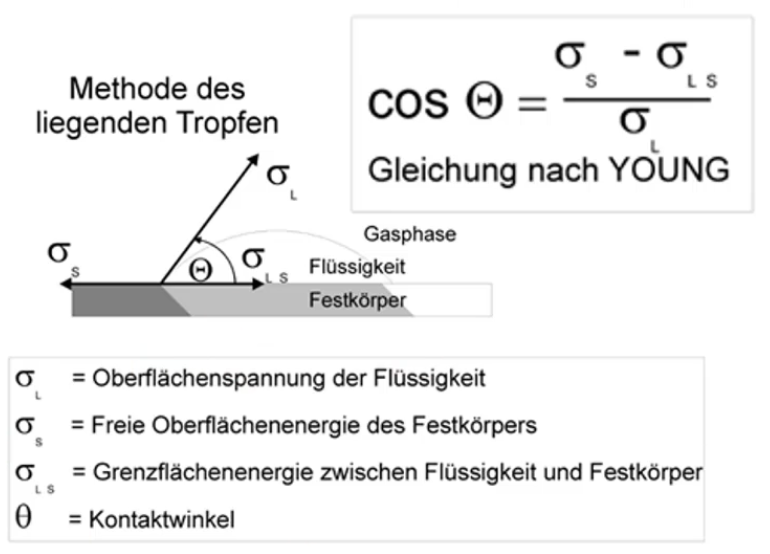
\includegraphics[width=8cm]{lec2/figures/young.png}	
\end{center}
\textbf{Neigungswinkel $\alpha$}\\
Neigungswinkel, ab welchem der Tropfen anfängt zu rollen. Weniger häufig angewandt zur Klassifizierung als Kontaktwinkel. 

\begin{center}
	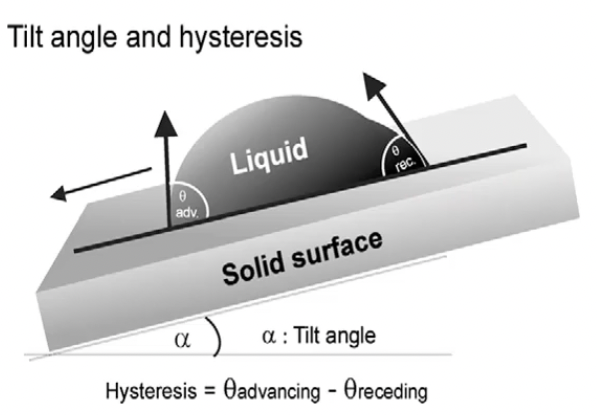
\includegraphics[width=8cm]{lec2/figures/neigungswinkel.png}	
\end{center}
Die Papillenartige Mikrostruktur beim Lotus-Blatt reduziert die effektive Fläche zwischen Flüssigkeit und Festkörper und beeinflusst dadurch die Grenzflächenenergie. Die folgenden \textbf{Typen des Benetzungsverhaltens} werden unterschieden \dangersign:

\begin{enumerate}
    \item \textbf{$\Theta < 90^\circ$}: hydrophil (benetzend)
    \item \textbf{$90^\circ < \Theta < 150^\circ$}: hydrophob (nicht benetzend)
    \item \textbf{$150^\circ \geq \Theta$}: superhydrophob
\end{enumerate}
Das Lotus-Blatt besitzt eine superhydrophobe Obefläche. Bei der Benetzung der verschiedenen Typen treten große dynamische Unterschiede bei der benetzenden Materie (z. B. Wasser) auf. 
\\\\
\textbf{Explizit klausurrelevant:} Einflussfaktoren des Benetzungsverhaltens \hintsign

\begin{itemize}
    \item Glatte vs. mikrostrukturierte Oberfläche
    \item Hydrophile vs. hydrophobe Oberfläche
    \item Oberflächenspannung des Wassers
    \item Kontaktfläche zwischen Tropfen und Oberfläche
    \item Lufteinschlüsse
\end{itemize}
\textit{Wie kommt es zustande, dass Strukturen superhydrophob sind und was muss erfüllt sein?}\\
Antwort: Mikrosturkutierung, Flüssigkeit muss passen, Oberfläche muss per se (chemisch) wasserabweisend sein.

\subsubsection{Der Selbstreinigungseffekt}

Der Selbstreinigungseffekt von Pflanzen ist \textbf{unabhängig von der Chemie} der Schmutzpartikel, setzt eine unbenetzbare Oberfläche voraus und wird durch folgende Zusammenhänge hervorgerufen \hintsign:

\begin{itemize}
    \item Reduzierte Kontaktfläche zwischen Pflanze und Partikeln durch \textbf{Mikrostrukturierung} (Haftkräfte von Partikeln auf Oberflächen auf 0,7 \% reduziert)
    \item \textbf{Unregelmäßige Strukturierung} reduziert die Kontaktfläche und die Haftkräfte weiter auf 0,07 \%
    \item Erhöhte Kontaktfläche der Partikel zum Wassertropfen
\end{itemize}

\begin{center}
	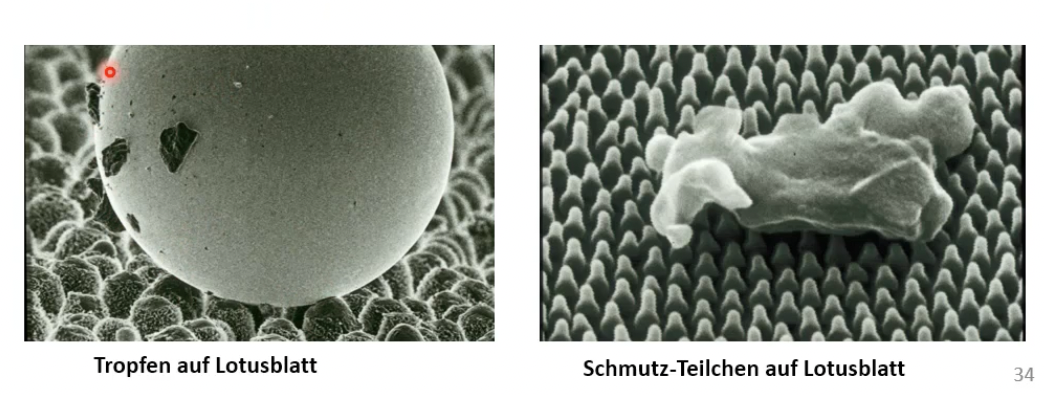
\includegraphics[width=12cm]{lec2/figures/selbstreinigung.png}	
\end{center}

\subsubsection{Herstellung von Papillen}

\textbf{Papillen} sind zapfenartige Vertiefungen und Erhebungen der Wachsschicht auf der Kutikula. Diese sind künstlich aufwändig herzustellen. In der Natur werden die Papillen vermutlich durch \textbf{Wachskristallbildung} konstruiert. Diese sind das Resultat von Selbstorganisationsprozessen und Wasserdampfdestillation über der Kutikula.

\begin{center}
	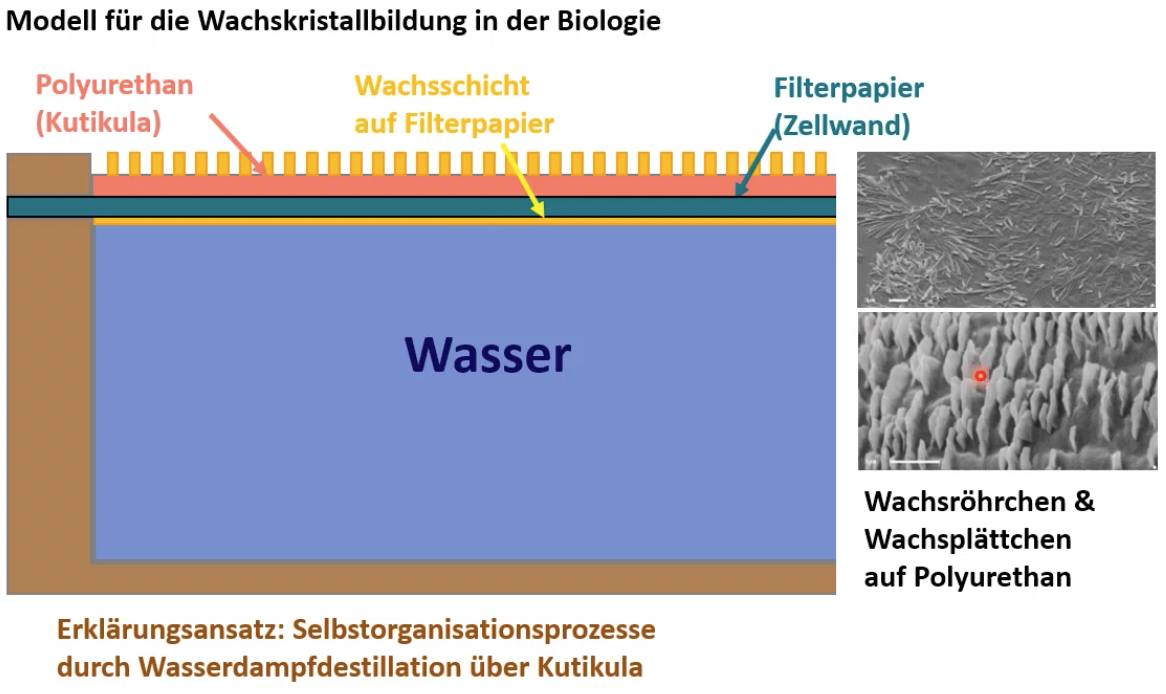
\includegraphics[width=12cm]{lec2/figures/wachskristallbildung.png}	
\end{center}
\subsubsection{Technische Anwendungen der Selbstreinigung - Der Lotus-Effekt}

Strukturen mit Lotus-Effekt sind immer \textbf{milchig} aufgrund der Papillen, welche das Licht unregelmäßig brechen und reflektieren. Herausforderungen entstehen durch Korrosion der künstlichen Wachsstrukturen, wodurch eine im Vergleich zu konventionellen Materialien vorzeitige Erneuerung notwendig wird, um den Effekt aufrechtzuerhalten. Dadurch meist kostenintensiver \dangersign. Bei der Pflanze wächst die Kutikula einfach nach, weshalb dies dort kein Problem darstellt.
\\\\
Anwendungsbeispiele für \textcolor{red}{selbstreinigende bzw. kontaktflächen-reduzierende künstliche Materialien} sind:

\begin{itemize}
    \item Fassadenfarbe mit Lotus-Effekt \dangersign
    \item Gläser (z.B.\ bei LKW-Mautsystem und Metallen)
    \item Sprays und Kunststoffbeschichtung (z.B.\ für Aufbewahrungsbehälter von teuren Flüßigkeiten)
    \item Textilien und Holzlacke (in Entwicklung)
    \item Honiglöffel (in Entwicklung)
    \item Dachziegel mit Titanoxid, das unter Einfluss von UV-Strahlung Elektronen freisetzt und Schmutz oxydiert (und dadurch zerstört)
    \item Kontaktflächenreduktion bei Hochtemperaturanwendungen (z.B.\ Bauteile in Hochöfen)
\end{itemize}

\subsection{Luftpolster unter Wasser}

Superhydrophobe Oberflächen bilden Luftkissen innerhalb der Papillen unter Wasser.
\\\\
Exkurs: Ein Beispiel für das Auftreten des Lotus-Effektes im Tierreich sind die \textbf{Sektrete und Drüsen von Streifenwanzen}, welche zur Feindabwehr und Abgabe von Pheromonen dienen sowie vor Mikroorganismen schützen. Da die Wanzen Luft über Tracheen (Vertiefungen über den ganzen Körper) aufnehmen und das Sekret auch für sie gitftig ist, müssen sie verhindern, dass es in die Tracheen gelangt. Die Lösung dafür ist ein gerichtetes und geführtes Abfließen über die Oberfläche, welches durch einen Lotus-Effekt erzielt wird.
\\\\
Die \textbf{unter Wasser glänzenden Luftpolster}, welche auf superhydrophobe Oberflächen schließen lassen, treten auch bei anderen Tierarten auf, wie z. B. der Südamerikanischen Wasserjagdspinne. Diese haben folgende Funktionen:

\begin{itemize}
    \item Schutzhülle gegen Feuchtigkeit und Temperatursprünge (vgl. Neoprenanzug)
    \item Versorgung mit Sauerstoff durch Tracheen-Atmung
\end{itemize}
In der Natur unterscheidet man die folgenden \textbf{drei Schwimmtypen}, welche teilweise aufgrund von Luftpolstern das Laufen auf dem Wasser erlauben:

\begin{enumerate}
    \item Passiv schwimmend (z. B. Schwimmfarn/ Salvinia)
    \item Aktive schwimmend (z. B. Wasserläufer)
    \item Tauchend (z. B. Wasserspinne)
\end{enumerate}
\textbf{Technische Anwendungen:}

\begin{itemize}
    \item Textilien für den Wassersport, die nicht nass werden \dangersign
    \item Beschichtung von Bootsrümpfen mit reibungsvermindernder Wirkung (reduzierter Strömungswiederstand)
\end{itemize}
\textbf{Fünf Prinzipien für permanente Luftschichten unter Wasser} \dangersign

\begin{enumerate}
    \item Hydrophobe Chemie
    \item Grobe Strukturen (z. B. Haare)
    \item Feinstruktur
    \item Hinterschneidung (damit Luftblasen  nicht aufgrund ihres Auftriebs entkommen)
    \item Elastizität (damit Luftblasen hinter Strukturen gehalten und nicht freigespült werden)
\end{enumerate}
Von diesen Prinzipien lassen sich die Feinstrukturen und Hinterschneidungen (Nanokavitäten) technisch nur äußerst schwer umsetzen. Es gelingt beispielsweise wasserabweisende Bademode herzustellen (hier können lediglich keine Feinstrukturen erzeugt werden).

\begin{center}
	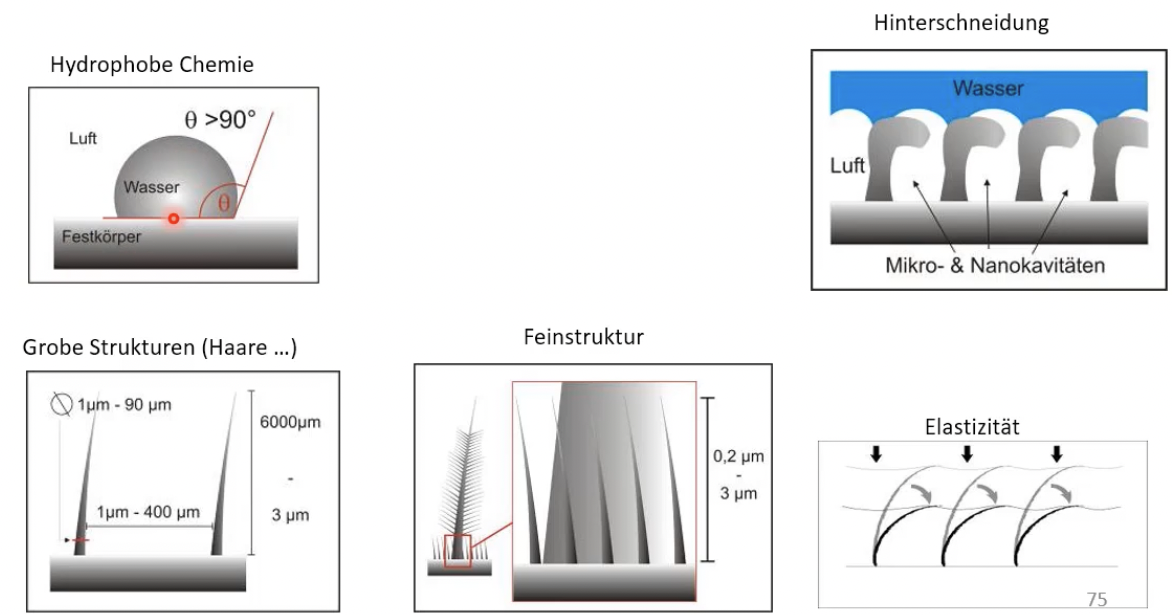
\includegraphics[width=14cm]{lec2/figures/prinizpien-luftschichten.png}	
\end{center}
Ein Prolbem, welches bei Luftpolstern unter Wasser auftreten kann, ist das sogennante \textbf{Salvinia-Problem}. Benannt ist es nach den verschiedenen Arten des Schwimmfarns von der Gattung Salvinia. Diese Pflanzen nutzen die Luftpolster, um ihre Blätter aufzuspannen und nahe der Wasseroberfläche zu halten (wo sie mehr Licht bekommen). Das Salvinia-Problem besteht darin, dass die Luft bei lokalen Druckinstabilitäten in Form von Luftblasen entweicht.
\\\\
Die Schwimmfarne der Gattung Salvinia verfügen außerdem über eine komplexe Zusammensetzung aus hydrophoben und hydrophilen Strukturen (an den Haarspitzen), wodurch sie sich an der Wasseroberfläche befestigen können. Dieser Effekt wird \textbf{Pinning} genannt.

\begin{center}
	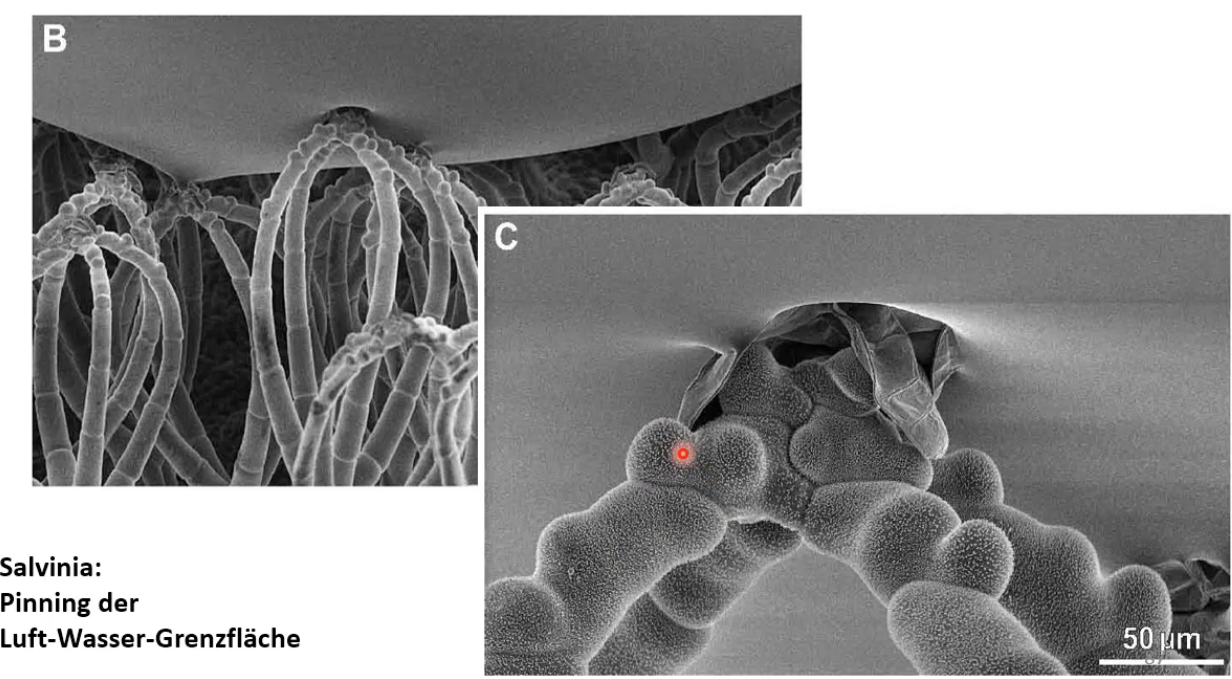
\includegraphics[width=14cm]{lec2/figures/pinning.png}	
\end{center}
Eine technische Anwendung stellt eine superhydrophobe Oberfläche für den Schiffsrumpf dar, die dann ein Luftpolster ausbildet (Salvinia-Effekt). Aktuell existieren auch z.B.\ Technologien, die dauerhaft Mikroluftblasen ausblasen, um Reibung zu verringern.

\subsection{Bionisches Antifouling: Bewuchsverhinderung im Meer}

Biogener (organischer) Bewuchs von Unterwasserkörpern durch Seepocken, Miesmuscheln und Algen verstärkt Korrosion und erhöht den Wasserwiederstand um bis zu 15 \%.
\\\\
Eine Lösung dafür aus der Natur ist ein \textbf{strukturiertes und elastisches System} nach Vorbild der Haihaut, welche aus Placoid-Schuppen besteht. Aus Experimenten mit unterschiedlich strukturierten und elastischen Gummi-Matten, welche im Meer versenkt wurden, wurde eine Haifischhaut-Farbe entwickelt, die \textbf{Bewuchs verringert} \dangersign.
\\\\
(\dangersign \textit{Welches Problem in der Schifffahrt? Was ist Antifouling? Was ist die konventionelle Lösung? Nenne eine Lösung aus der Bionik + Funktionsprinzip})











\section{Bionische Oberflächen: Haftung und Antihaftung nach dem Vorbild der Natur}

\subsection{Superhydrophile Oberflächen}

\subsubsection{Am Beispiel der Wüstenechsen}

Wenn Wassertropfen die Oberfläche benetzen (sodass wir den Kontaktwinkel nicht mehr messen können), deutet das auf superhydrophile Oberflächen hin. Dies sehen wir z.B.\ bei den Schuppen von Wüstenechsen wie dem Dornenteufel (zweite Reihe im nächsten Bild links), der Texas-Krötenechse (dritte Reihe), etc. In der ersten Reihe ist zum Vergleich ein Wassertropfen auf den Schuppen einer nicht in der Wüste lebenden Eidechsenart dargestellt. Bei dieser Art hat sich die Funktion der hydrophilen Oberfläche nicht entwickelt.

\begin{center}
    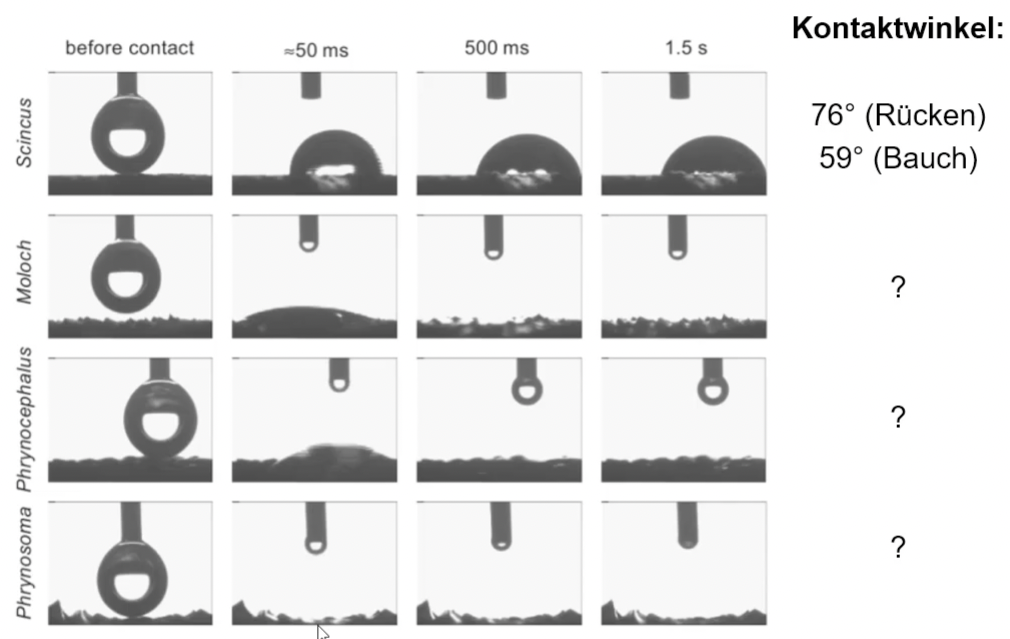
\includegraphics[width=10cm]{lec3/figures/Benetzung.png}
    \hfill
    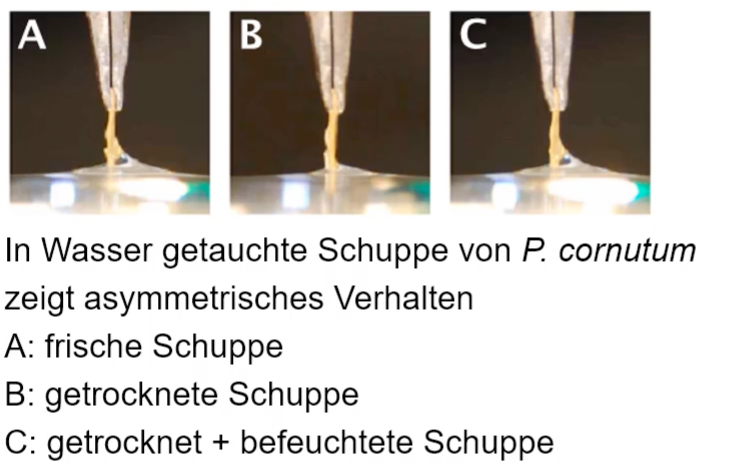
\includegraphics[width=6cm]{lec3/figures/Tauchen.png}
\end{center}
In dem rechten Bild ist ein Versuch zu sehen, bei dem 3 Schuppen in Wasser getaucht werden. Je nach Typ entstehen dabei unterschiedliche Kontaktwinkel, wobei der Innenbereich der Schuppe immer größere Kontaktwinkel als der Außenbereich hat. Da dieses Verhalten mit der unterschiedlichen Oberflächenstruktur zwischen Innen- und Außenbereich (Außenbereich zeigt Honigwaben-Mikrostruktur, Innenbereich nicht) korelliert, können wir hier die Ursache für den Effekt \textit{vermuten}.\\

Um diesen Zusammenhang nun zu beweisen, müssten wir genug kritische Versuche durchführen, welche die Vermutung nicht widerlegen. Ein möglicher Versuch, ist die Abformung der Mikrostrukturen mit Harz. Im nächsten Bild benetzt der Wassertropfen auf der abgeformten Funktionsoberfläche das Harz (oben), während der Tropfen auf der strukturlosen, ungeformten Rückseite des Harzes einfach abfließt (unten).

\begin{center}
    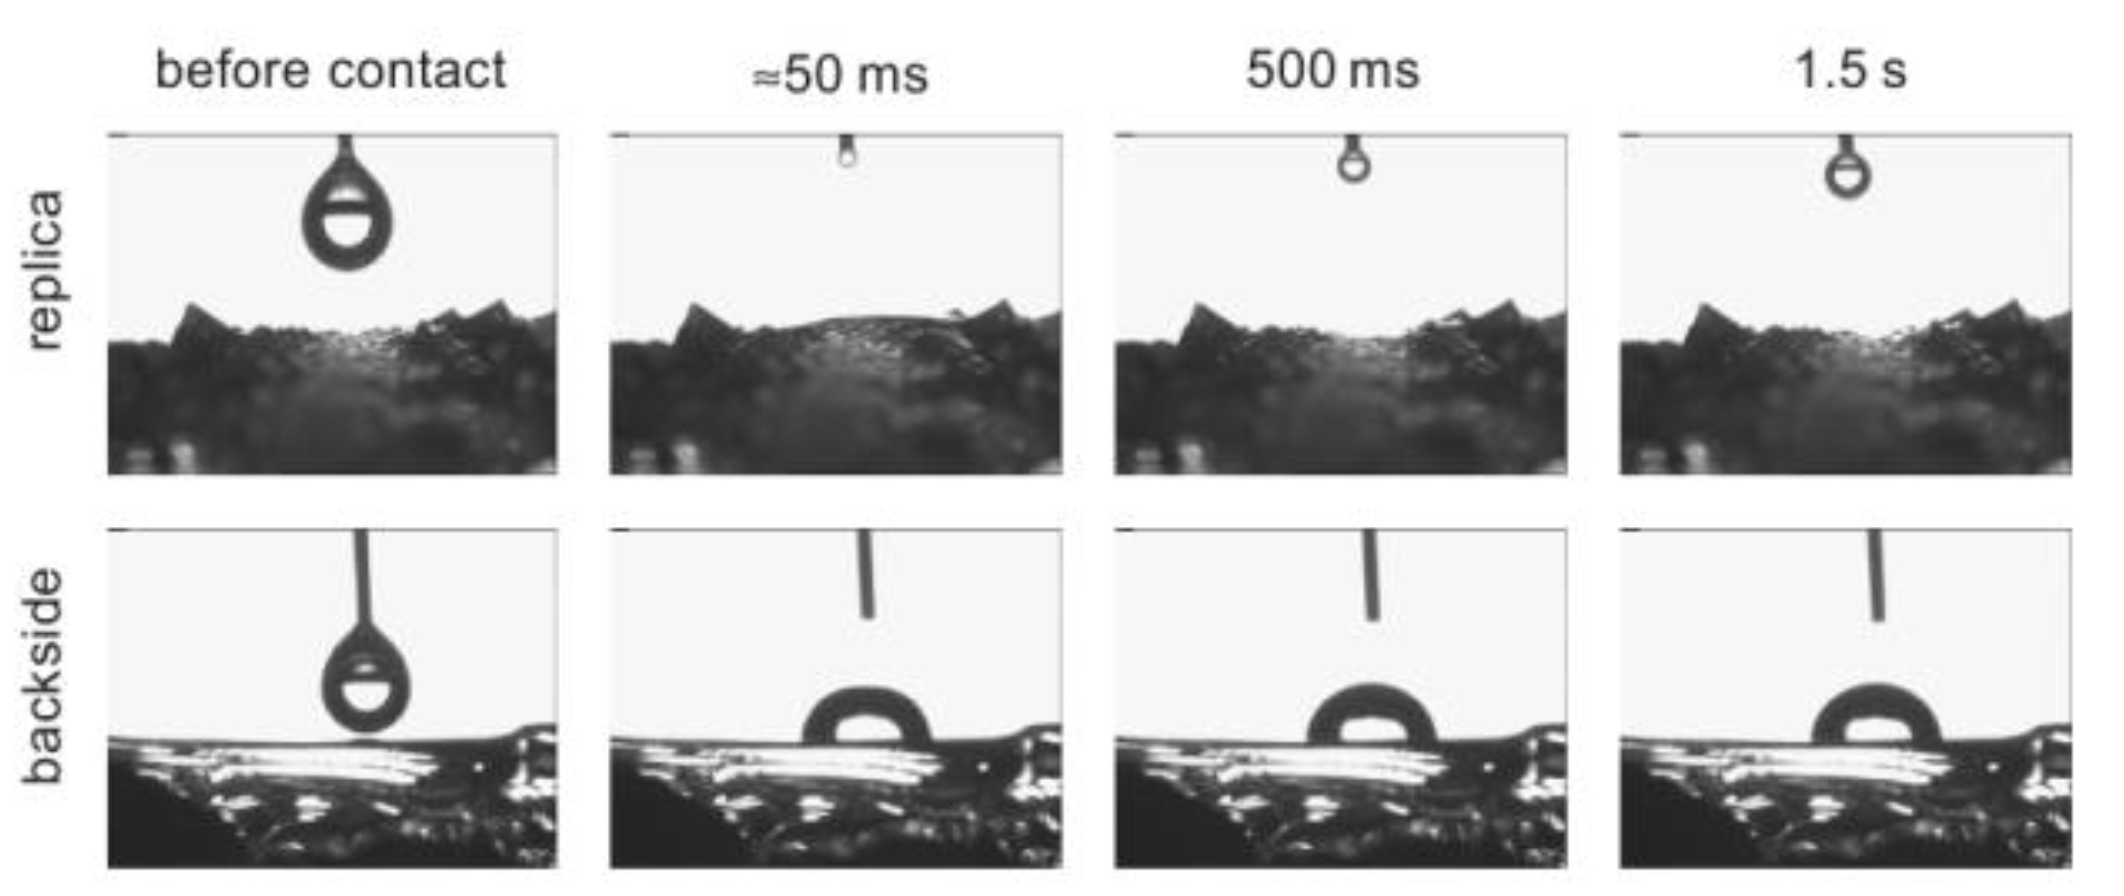
\includegraphics[width=10cm]{lec3/figures/Resin.png}
\end{center}

\paragraph{Wie kommt der richtungspezifische Transport von Flüssigkeit auf den Schuppen zustande?} Bei gewissen Arten wird Flüssigkeit Richtung Maul transportiert. Der Zwischenschuppen-Kanal (im linken Bild unten b; Spalt zwischen zwei Schuppen) weißt kleine Kerben (c) auf, deren Querschnit in Richtung des Mauls immer geringer wird. Es ergibt sich ein sägezahnförmiger Kanal (rechtes Bild). Die Flüssigkeit fließt aufgrund der Kapillarwirkung stets in Richtung der Verengung. (\dangersign \textit{Wie funktioniert der Richtungstransport von Wasser bei der Texas-Krötenechse?}) 

\begin{center}
    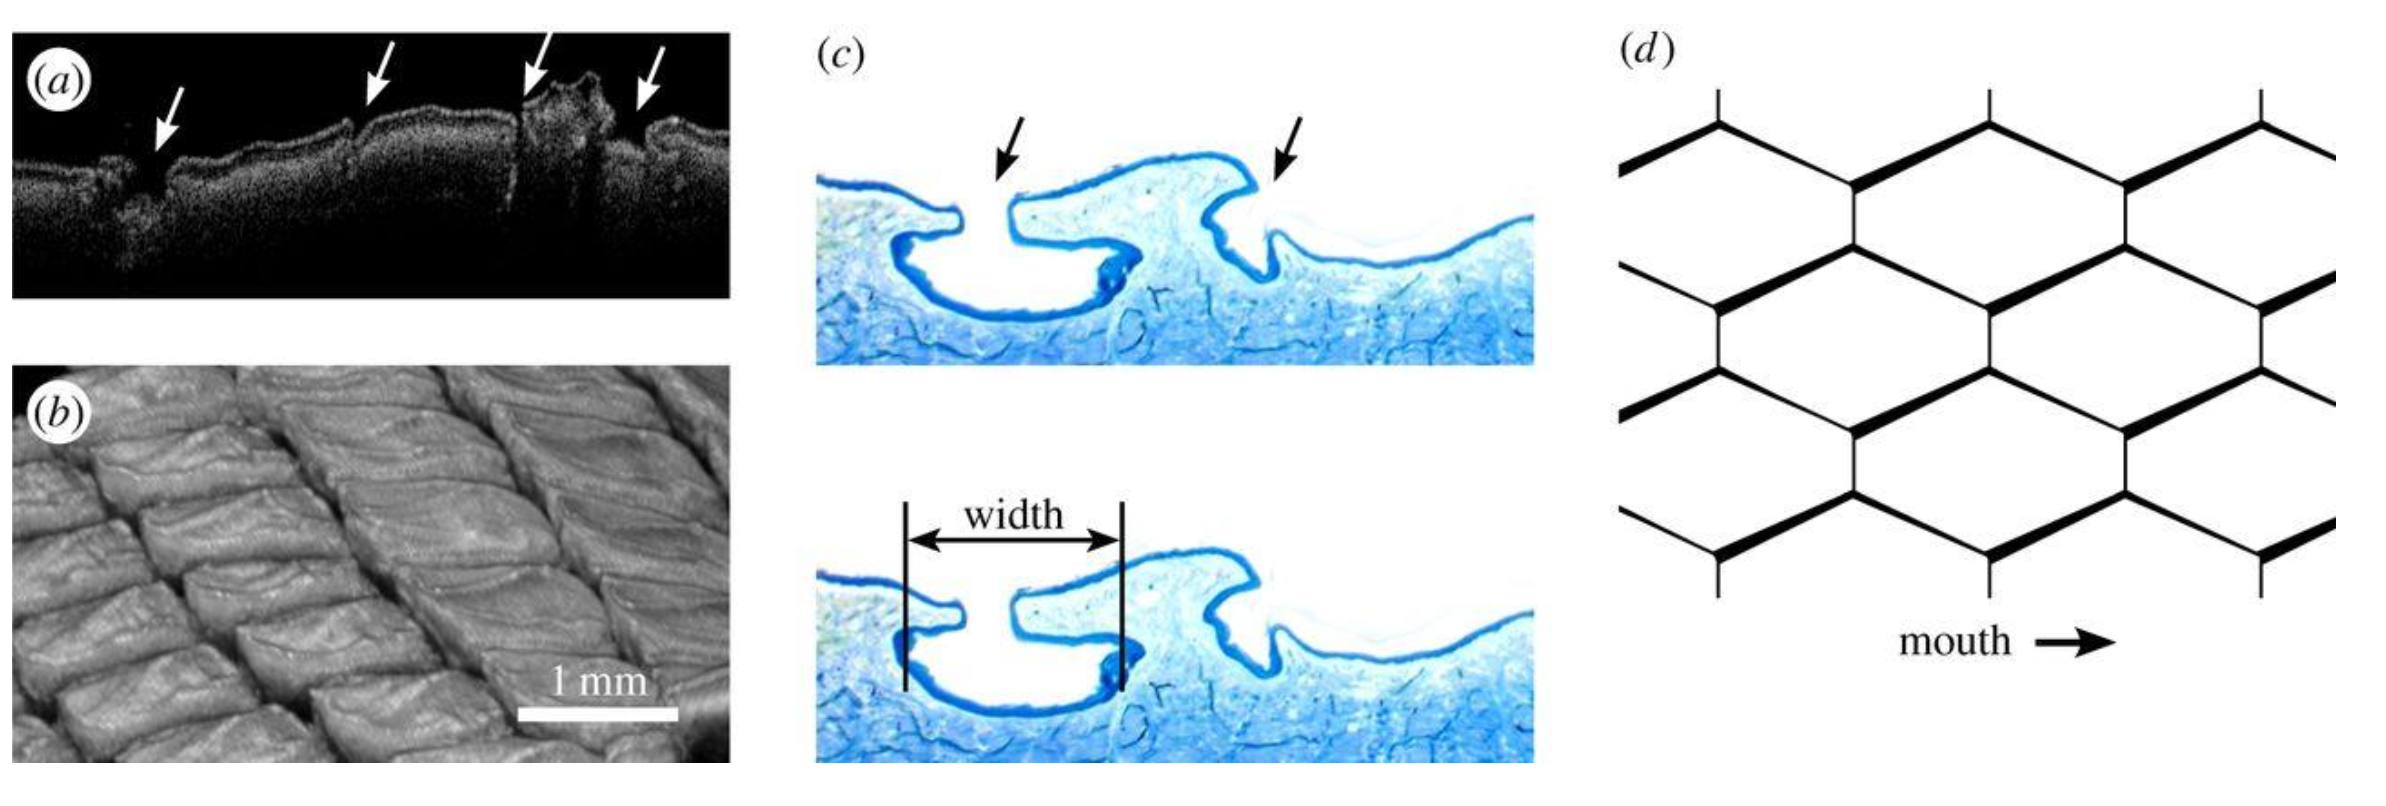
\includegraphics[width=10cm]{lec3/figures/Kerben.png}
    \hfill
    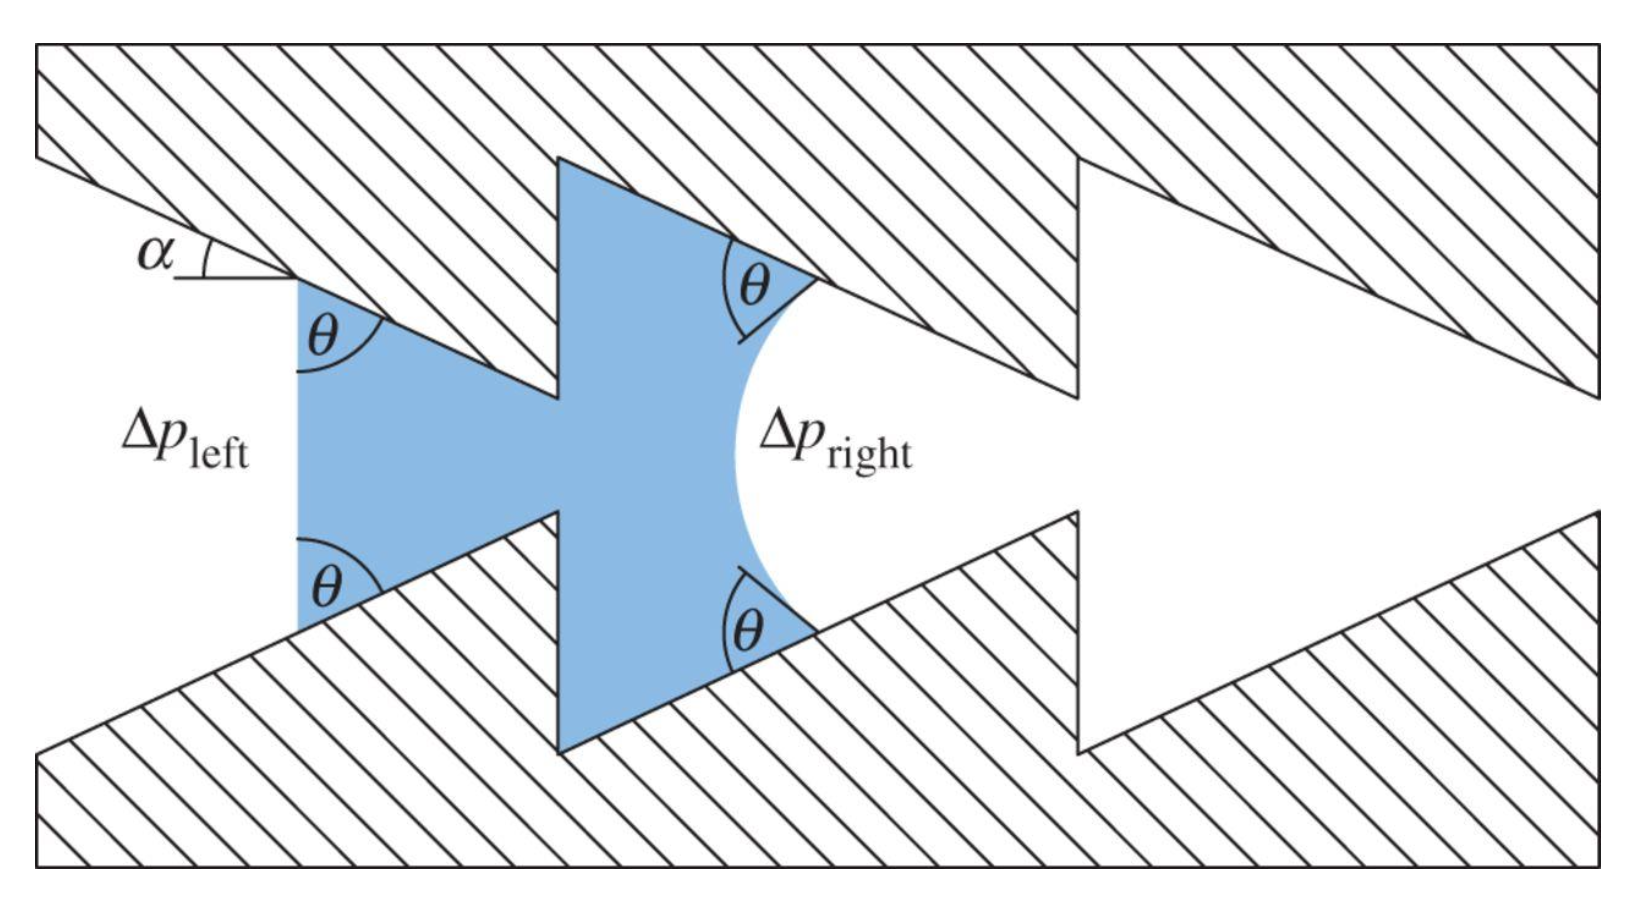
\includegraphics[width=6cm]{lec3/figures/Kanal.png}
\end{center}

\textit{Wie lässt sich das technisch nutzen} \dangersign? Sportbekleidung, die den Schweiß in Körperbereiche bringt, die gekühlt werden sollen. Oder zur verbesserten Verteilung von Flüssigkeiten auf Metall z.B.\ Öl, Kühlmittel (Einbringung per Laserstrahlstrukturierung, etc.) 

\subsubsection{Modelle zur Beschreibung des Benetzungsverhaltens}

Das \textbf{Wenzel-Modell} versucht den \textcolor{red}{Einfluss von Mikrostrukturierung auf das Benetzungsverhalten} zu erklären \dangersign, wobei die Flüssigkeit zwischen den Mikrostrukturen eindringt. Dabei errechnet sich der Kontaktwinkel der strukturierten Oberfläche $\theta_m$ nach:

$$\cos \theta_m = r \cos \theta,$$

wobei $\theta$ der Kontaktwinkel der glatten Oberfläche und $r$ der Quotient aus tatsächlicher Fläche (``von oben sichtbare Fläche'') und projizierter Fläche (ges. Oberfläche der Mikrostrukturen) ist. Die \textbf{Strukturierung führt bei chemisch hydrophilen Oberflächen dazu, dass die superhydrophil werden}. Allerdings kann das Modell bei den beschriebenen Echsenarten das Benetzungsverhalten nicht erklären. Wenn der Wassertropfen hängen bleibt ($\Longrightarrow$ Petal-Effekt, superhydrophobe Oberfläche die das Abrollen des Tropfen verhindert).\\

Bei dem \textbf{Cassie-Modell} sprechen wir von einer heterogenen Benetzung. Hier dringt die Flüssigkeit nicht zwischen die Mikrostrukturen ein ($\Longrightarrow$ Lotus Effekt, superhydrophobe Oberfläche).\\

Bei der \textbf{Cassie-Imprägnierung} dringt die \textcolor{red}{Flüssigkeit auch zischen die Mikrostrukturen ein, breitet sich darüber aus} \dangersign und macht die Oberfläche \textbf{superhydrophil}. Bei den Eidechsen kann mit dem Cassie-Impregnierungs-Modell das superhydrophile Benetzungsverhalten erklärt werden.

\begin{center}
    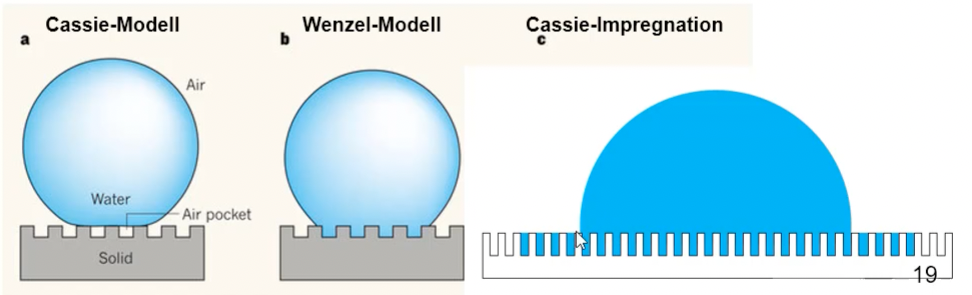
\includegraphics[width=10cm]{lec3/figures/wenzel_cassie.png}
\end{center}

\subsection{Lagebezeichnungen}
In der Biologie werden bestimmte \textbf{Lagebezeichnungen} verwendet, um die Lage von Körperteilen zu beschreiben:
\begin{itemize}
    \item Medial = Innen
    \item Lateral = Außen
    \item Dorsal = Rücken (Bspl. Dorsalschuppen)
    \item ventral = Bauch
    \item caudal = Schwanz
    \item cranial = Kopf
    \item proximal = Nah am Körper
    \item distal = Weit weg vom Körper
\end{itemize}

\subsection{Reversible Anhaftung nach dem Gecko- und Insektenfußprinzip}

\textbf{Adhesion} = trockenes Kleben (reversible Anhaftung).

Die Komplexität der Strukturierung nimmt hierarchisch von der Makro- zur Nanoebene zu \dangersign. Sowohl bei Geckos, als auch bei manchen Insekten findet sich diese hierarchische Gliederung und das Anhaften an unterschiedlichen Oberflächen. Feine Strukturen (\textcolor{red}{Lamella $\rightarrow$ Setae $\rightarrow$ Spatulae} im Bild unten) liegen eng an der Kontur der Oberfläche an, sodass sich van der Waals-Kräfte einstellen. Dieser schwache Anziehungseffekt stärkt die Adhesion.

\begin{center}
    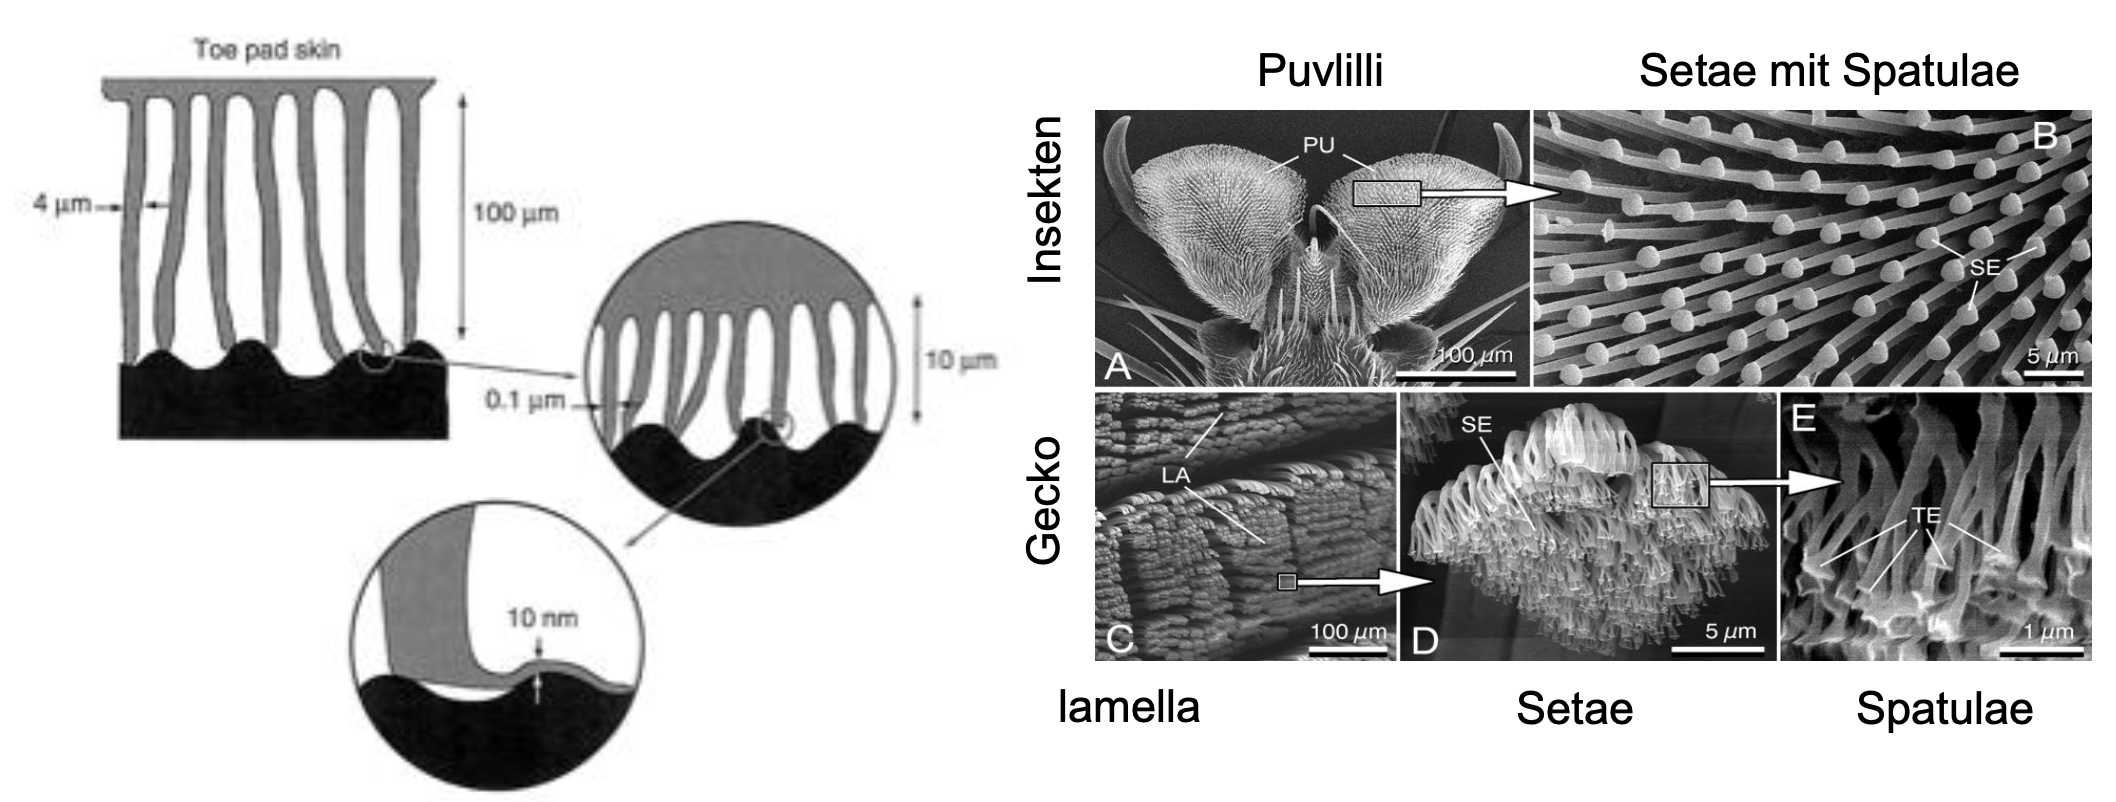
\includegraphics[width=10cm]{lec3/figures/vanderwaals.png}
    \hfill
    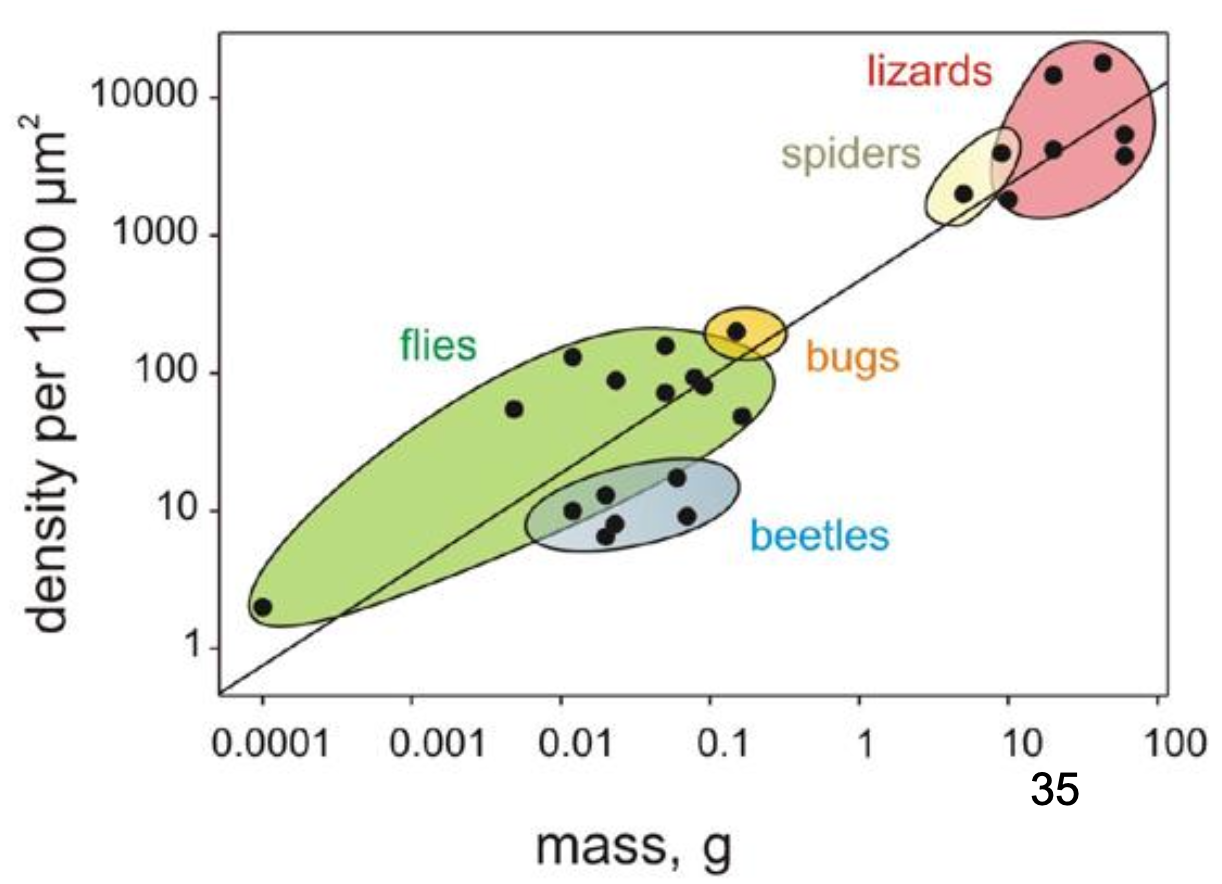
\includegraphics[width=6cm]{lec3/figures/setadichte.png}
\end{center}
Untersuchungen zeigen: Je schwerer das Tier ist, desto höher ist die Seta-Dichte, um das Gewicht des Tieres zu halten (siehe das Bild oben rechts). 
\\\\
\textit{Eine technische Anwendung}\dangersign: Das \textbf{``Gecko-Tape'' besitzt eine Oberfläche mit Setae-Strukturen}. Dabei stellte sich heraus, dass Setae mit \textbf{Pilzkopf-Form} (dem Kartoffelkäfer nachgearmt) besser haften.

\begin{center}
    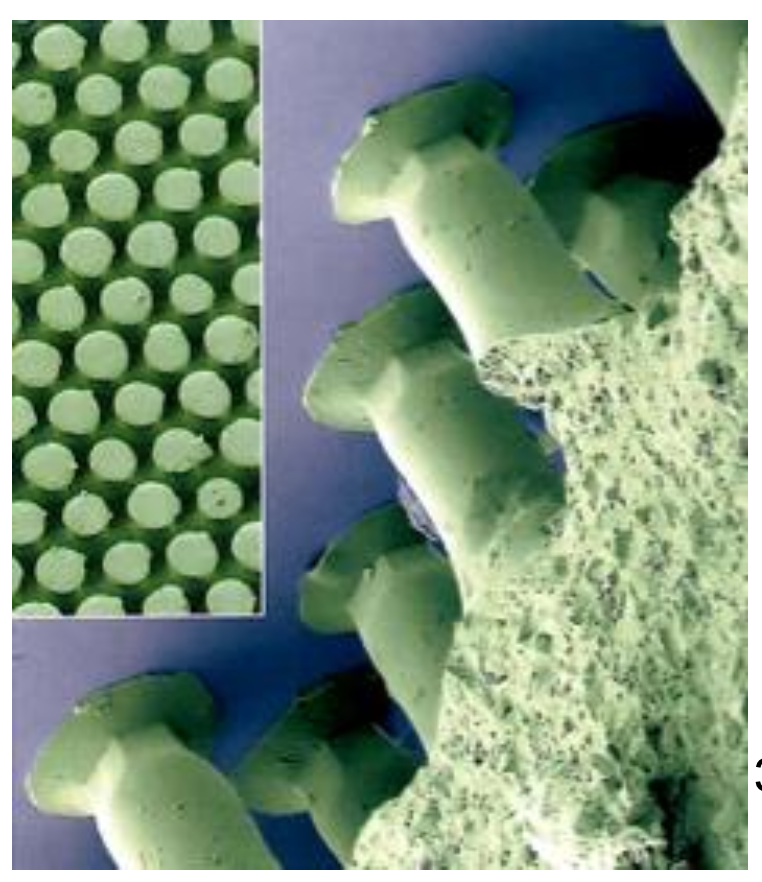
\includegraphics[width=3cm]{lec3/figures/pilzkopfform.png}
\end{center}






\section{Bionische Oberflächen 2}

\subsection{Temporäre Haftsysteme mit regulierbaren Hafteigenschaften}

\textit{Beispiel 1: Klettverschluss.} Nach dem Vorbild von Klettfrüchten, deren Samen durch das Klettsystem (kleine Widerhaken) an Tieren anhaften und sich verbreiten. Als biologisches Vorbild dienen die Hakenstrukturen von Spreizklimmern.
\\
\textit{Verbesserungen vom Klettverschluss}:
\begin{itemize}
    \item Mit richtungssabhängigen, variablen \& richtungsabhängigen Hafteigenschaften: Pneumatische Schläuche öffnen die Haken unter Druck ($\rightarrow$ Haftung).
    \item \textbf{Anisotrope (richtungsunabhängige) Haftung} \dangersign: Je nach Bewegungsrichtung Haften oder Gleiten. Beste Eigenschaften, wenn weiche Fasern in steife Fasern greifen $\rightarrow$ zB für Posterclips.
\end{itemize}

\begin{center}
    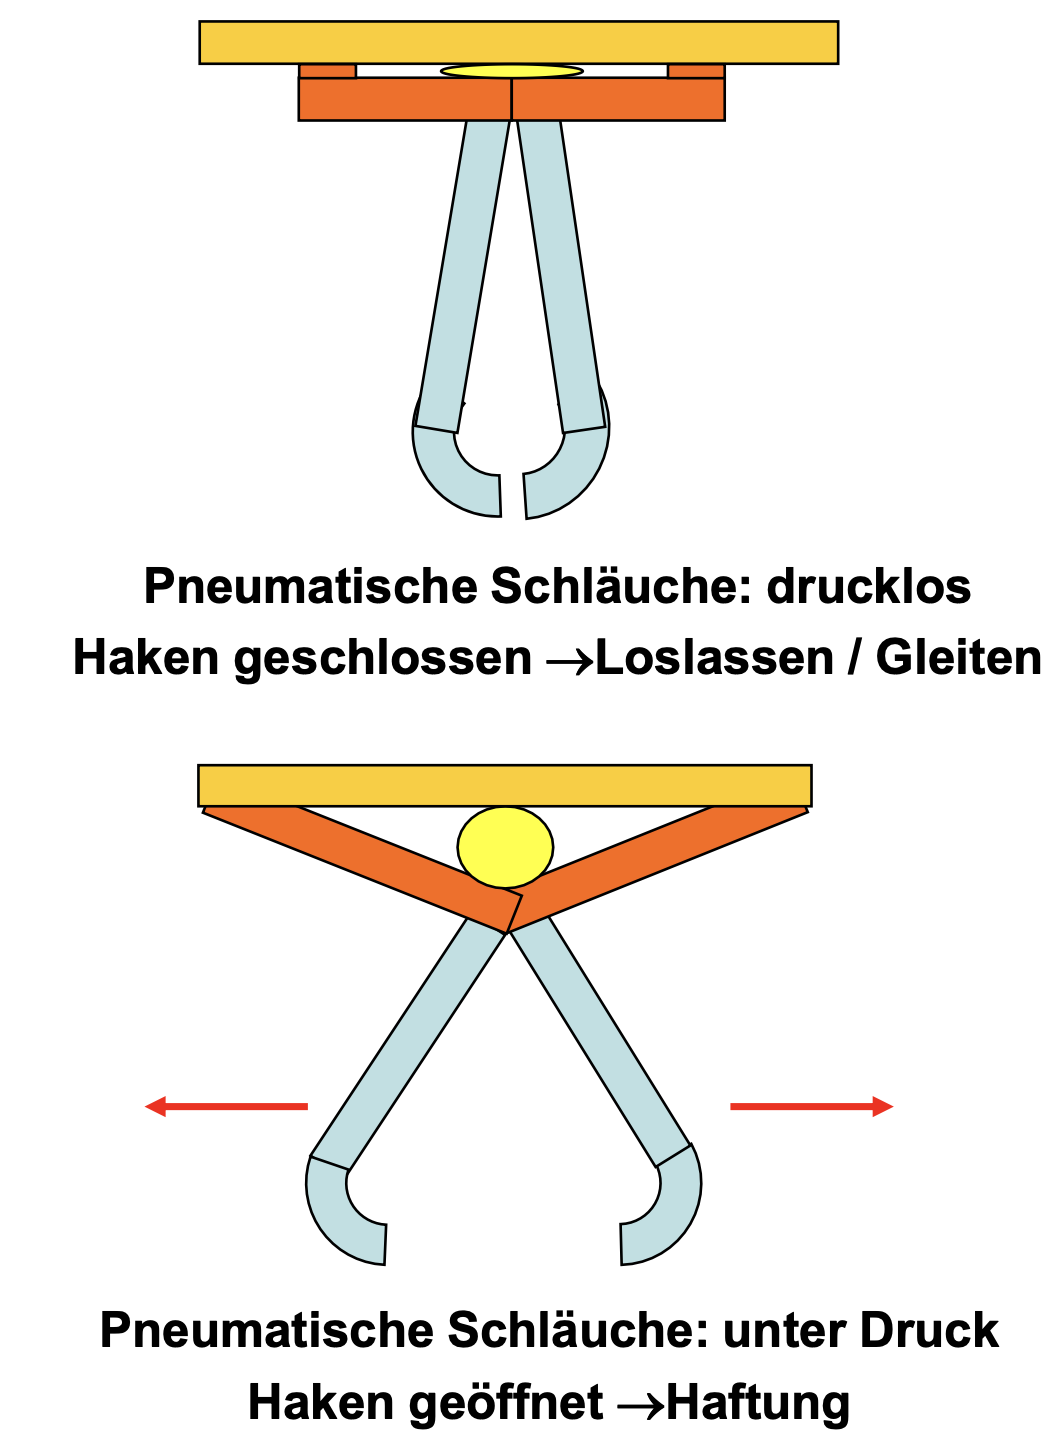
\includegraphics[width=4cm]{lec4/figures/pneumatik.png}
    \hfill
    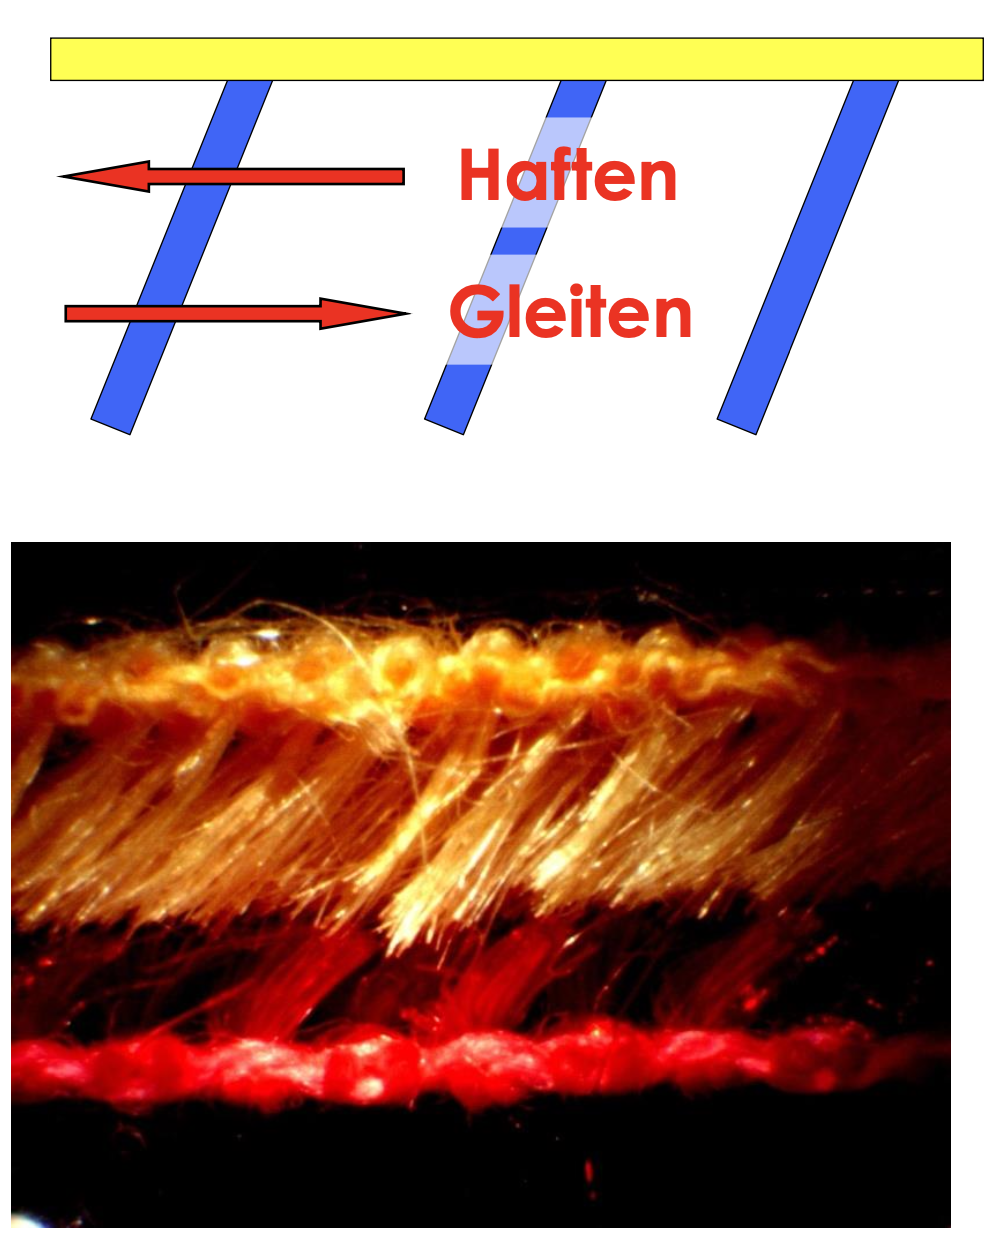
\includegraphics[width=4cm]{lec4/figures/anisotropes_haften.png}
\end{center}

\subsection{Permanente Haftsysteme mit hoher Haftkraft}

\textbf{Beispiel 1: Haftwurzeln beim Efeu.} Das Wurzelhaar wächst in Spalten ein, nimmt mit dem Substrat Kontakt auf und klappt durch Eintrocknen um $\rightarrow$ Haftung. In den Haaren sind die Fasern in 30-40° zur Längsrichtung orientiert, aber in der Sitze in 60° $\rightarrow$ verursacht das Abknicken in der Spitze. Zudem hat der Efeu ``Klebekapseln'' die die Wurzelhaare an das Substrat binden. Bei Kraft-Weg-Messungen an Hauswänden zeigt sich ein abgestuftes Versagen. An Baumborken werden höhere Haftkräfte erreicht, wobei durch das weichere Substrat schnelleres Versagen eintritt.
\\
(\dangersign\textit{Wie haftet Efeu? Warum knickt es ab? Wo haftet es besonders gut? $\rightarrow$ raue Oberflächen hoher Festigkeit})

\begin{center}
    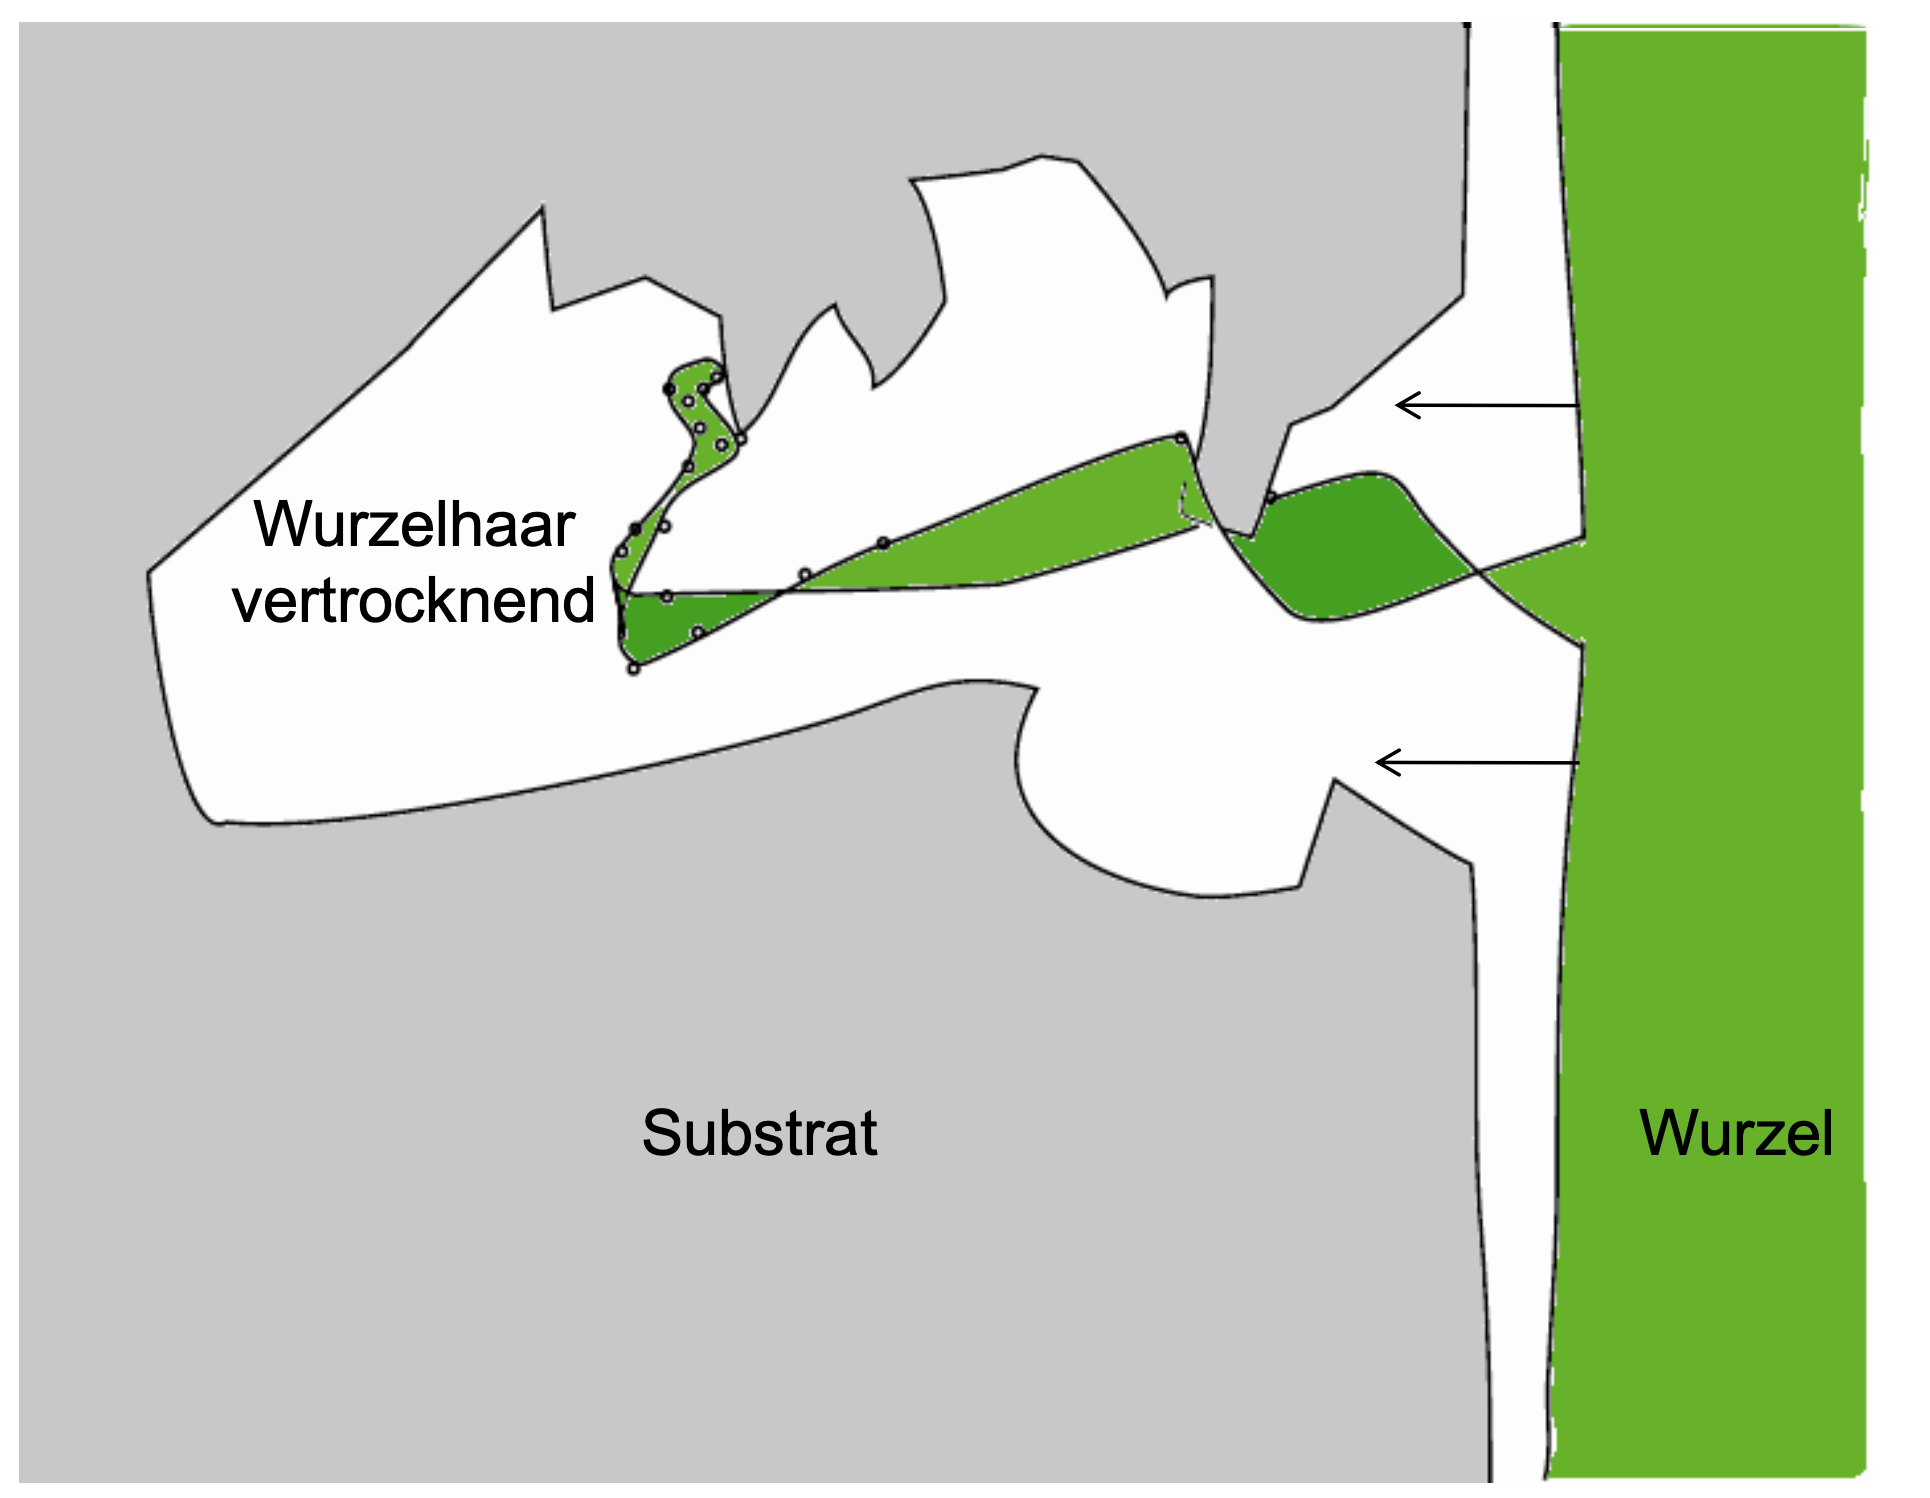
\includegraphics[width=5cm]{lec4/figures/efeu_haar.png}
    \hfill
    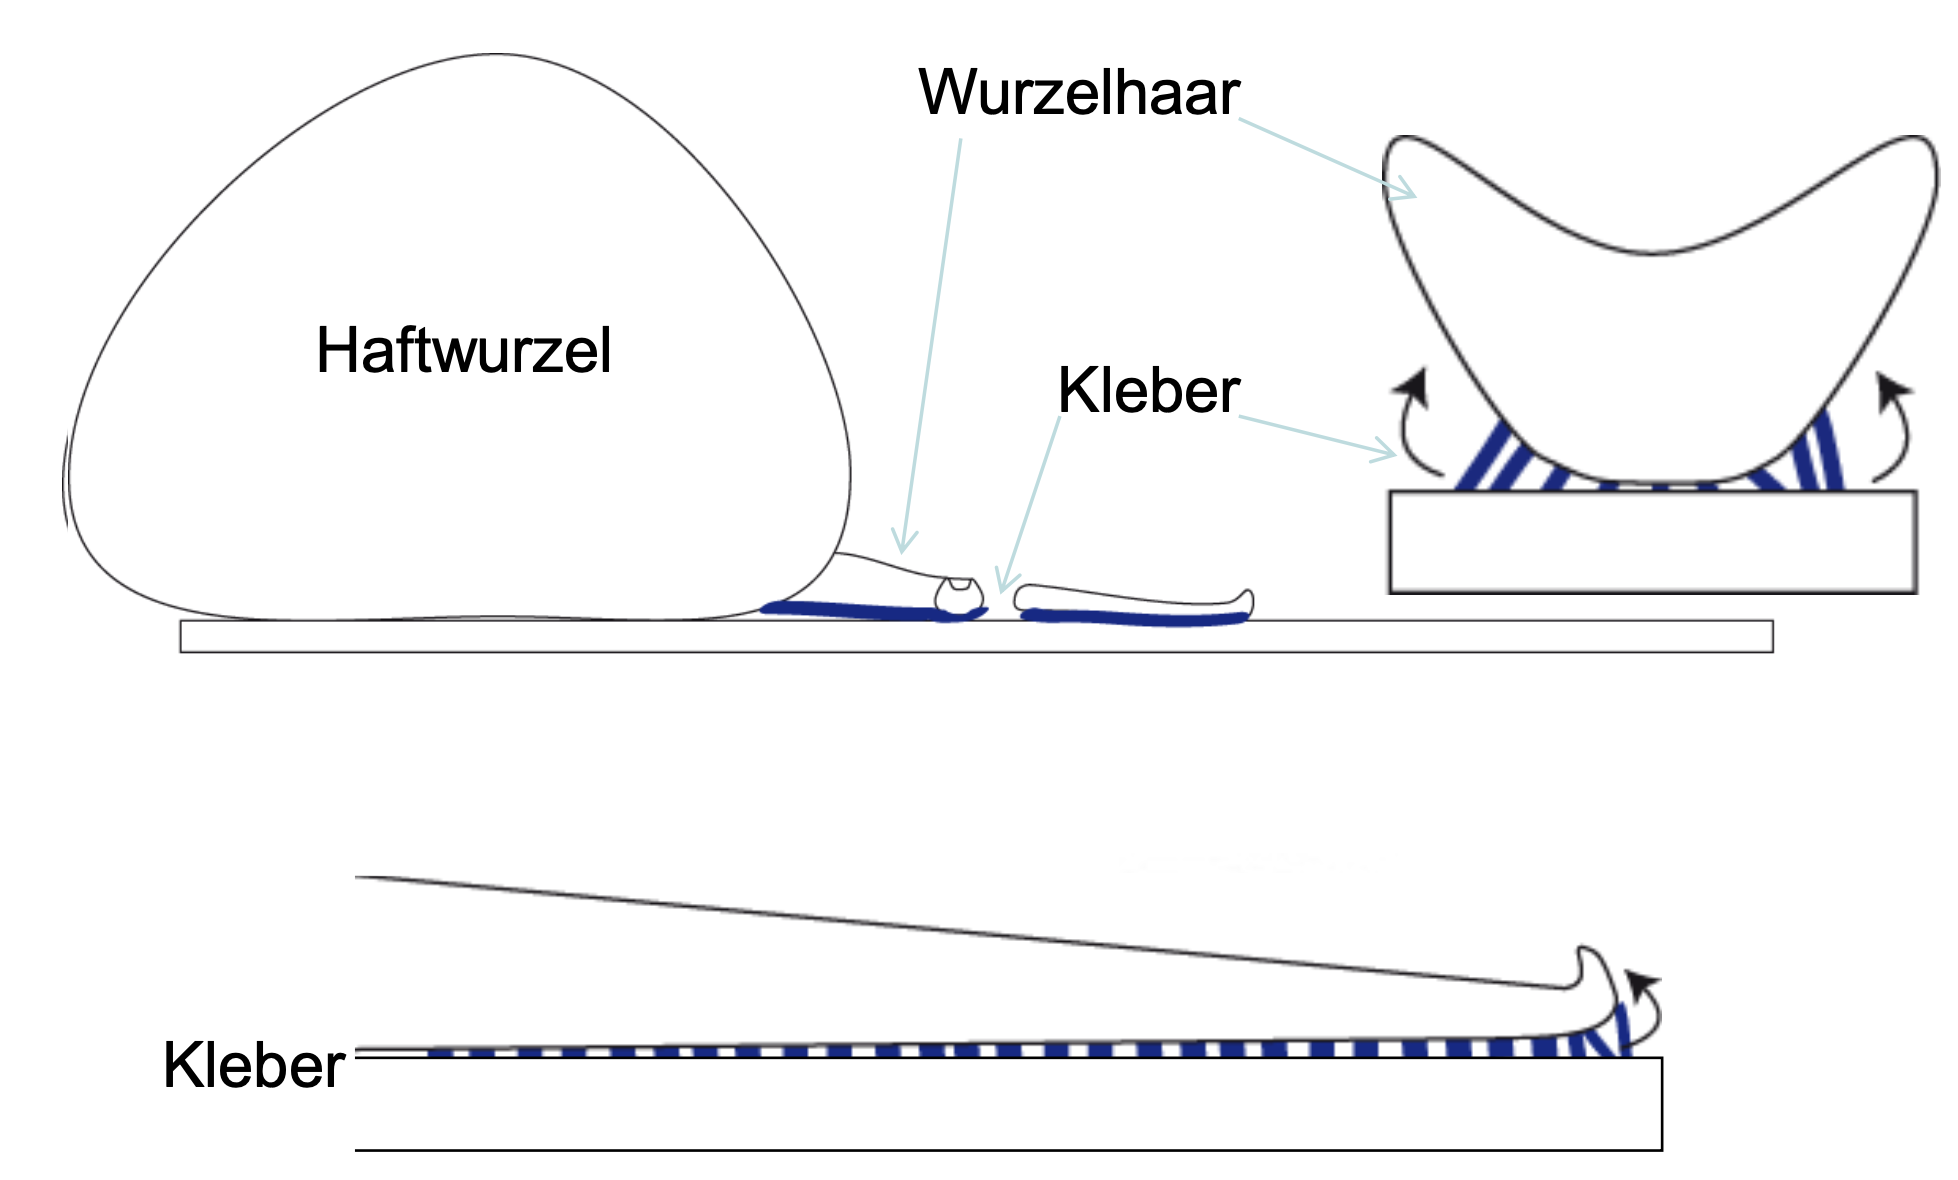
\includegraphics[width=5cm]{lec4/figures/efeu_kleber.png}
    \hfill
    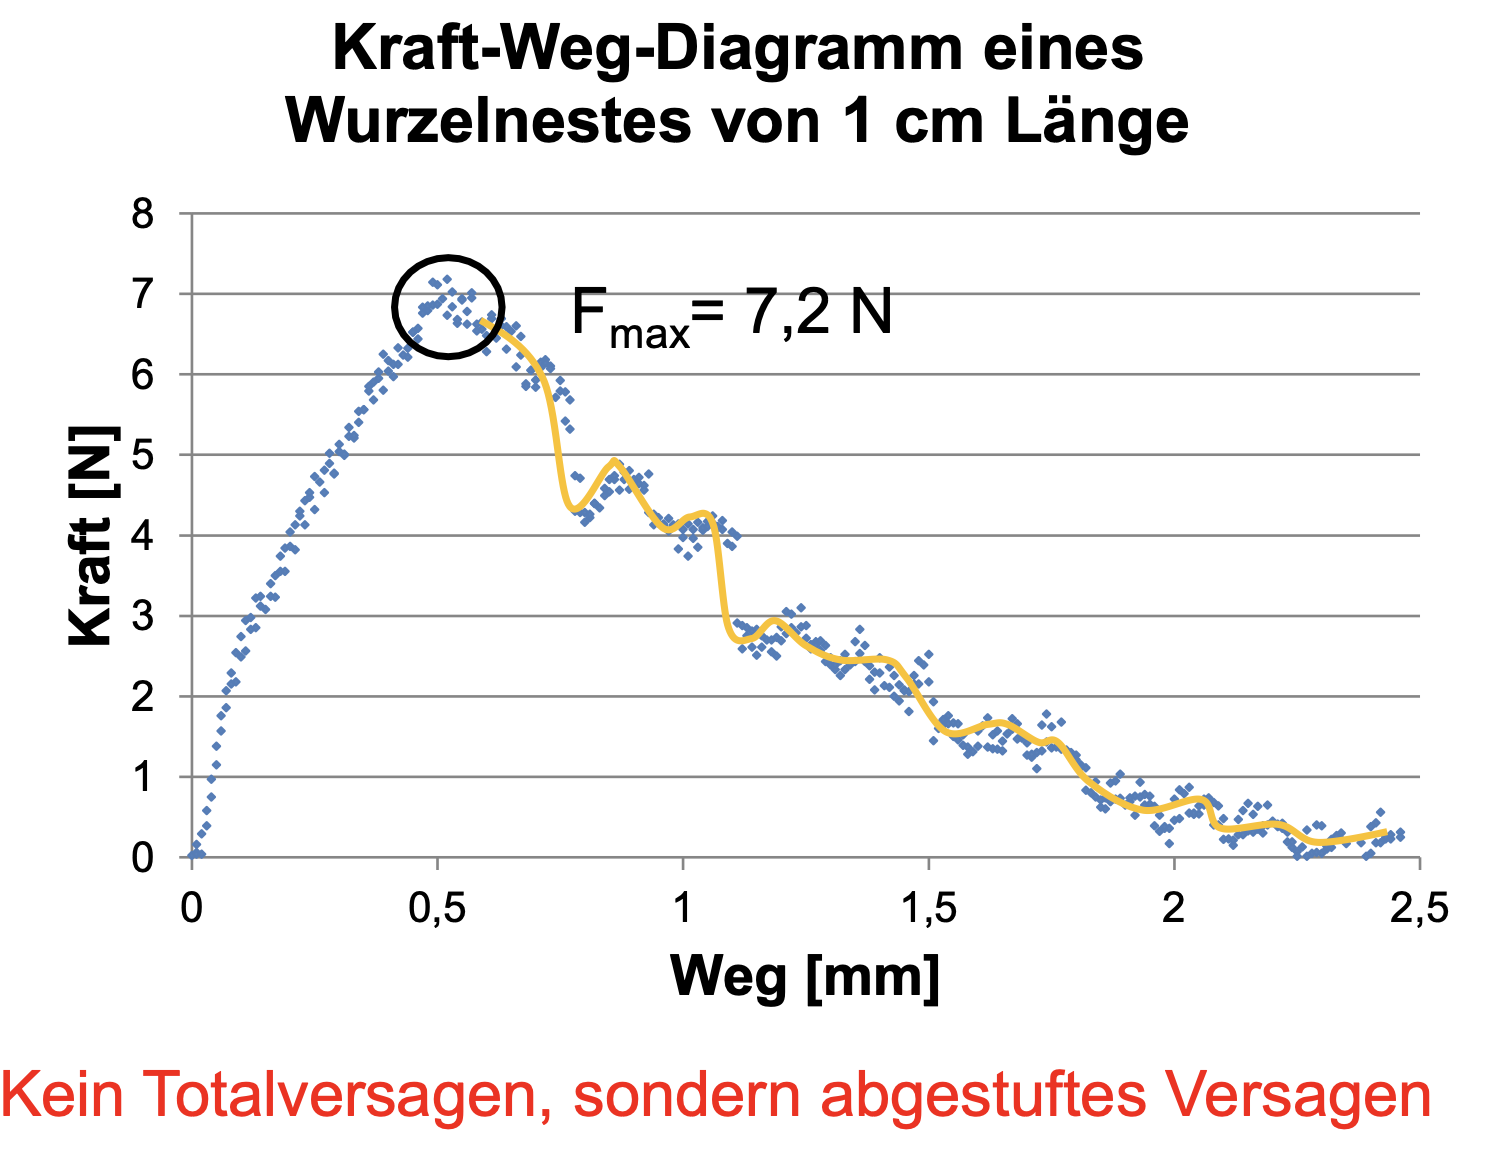
\includegraphics[width=5cm]{lec4/figures/efeu_versagen.png}
\end{center}
\textbf{Beispiel 2: Haftpads beim Wilden Wein.} Ranken wachsen $\rightarrow$ kommen in Kontakt zum Substrat $\rightarrow$ Haftpads bilden Hüte aus $\rightarrow$ Haftpads verholzen. Im Gegensatz zum Efeu zeigt das Kraft-Weg-Diagramm beim Wilden Wein Totalversagen. Je nach Art des Substrats stellen sich dabei unterschiedliche Versagensbilder ein (auf Putz versagt eher das Substrat und auf Aluminium versagt eher die Kappe).

\textit{Bionische Umsetzung:} Es wird probiert, Kleber in die Kontaktzone zweier Oberflächen so einzubringen, sodass die Kraftleitungsgeometrie der Haftpads beim Wilden Wein imitiert wird.

\begin{center}
    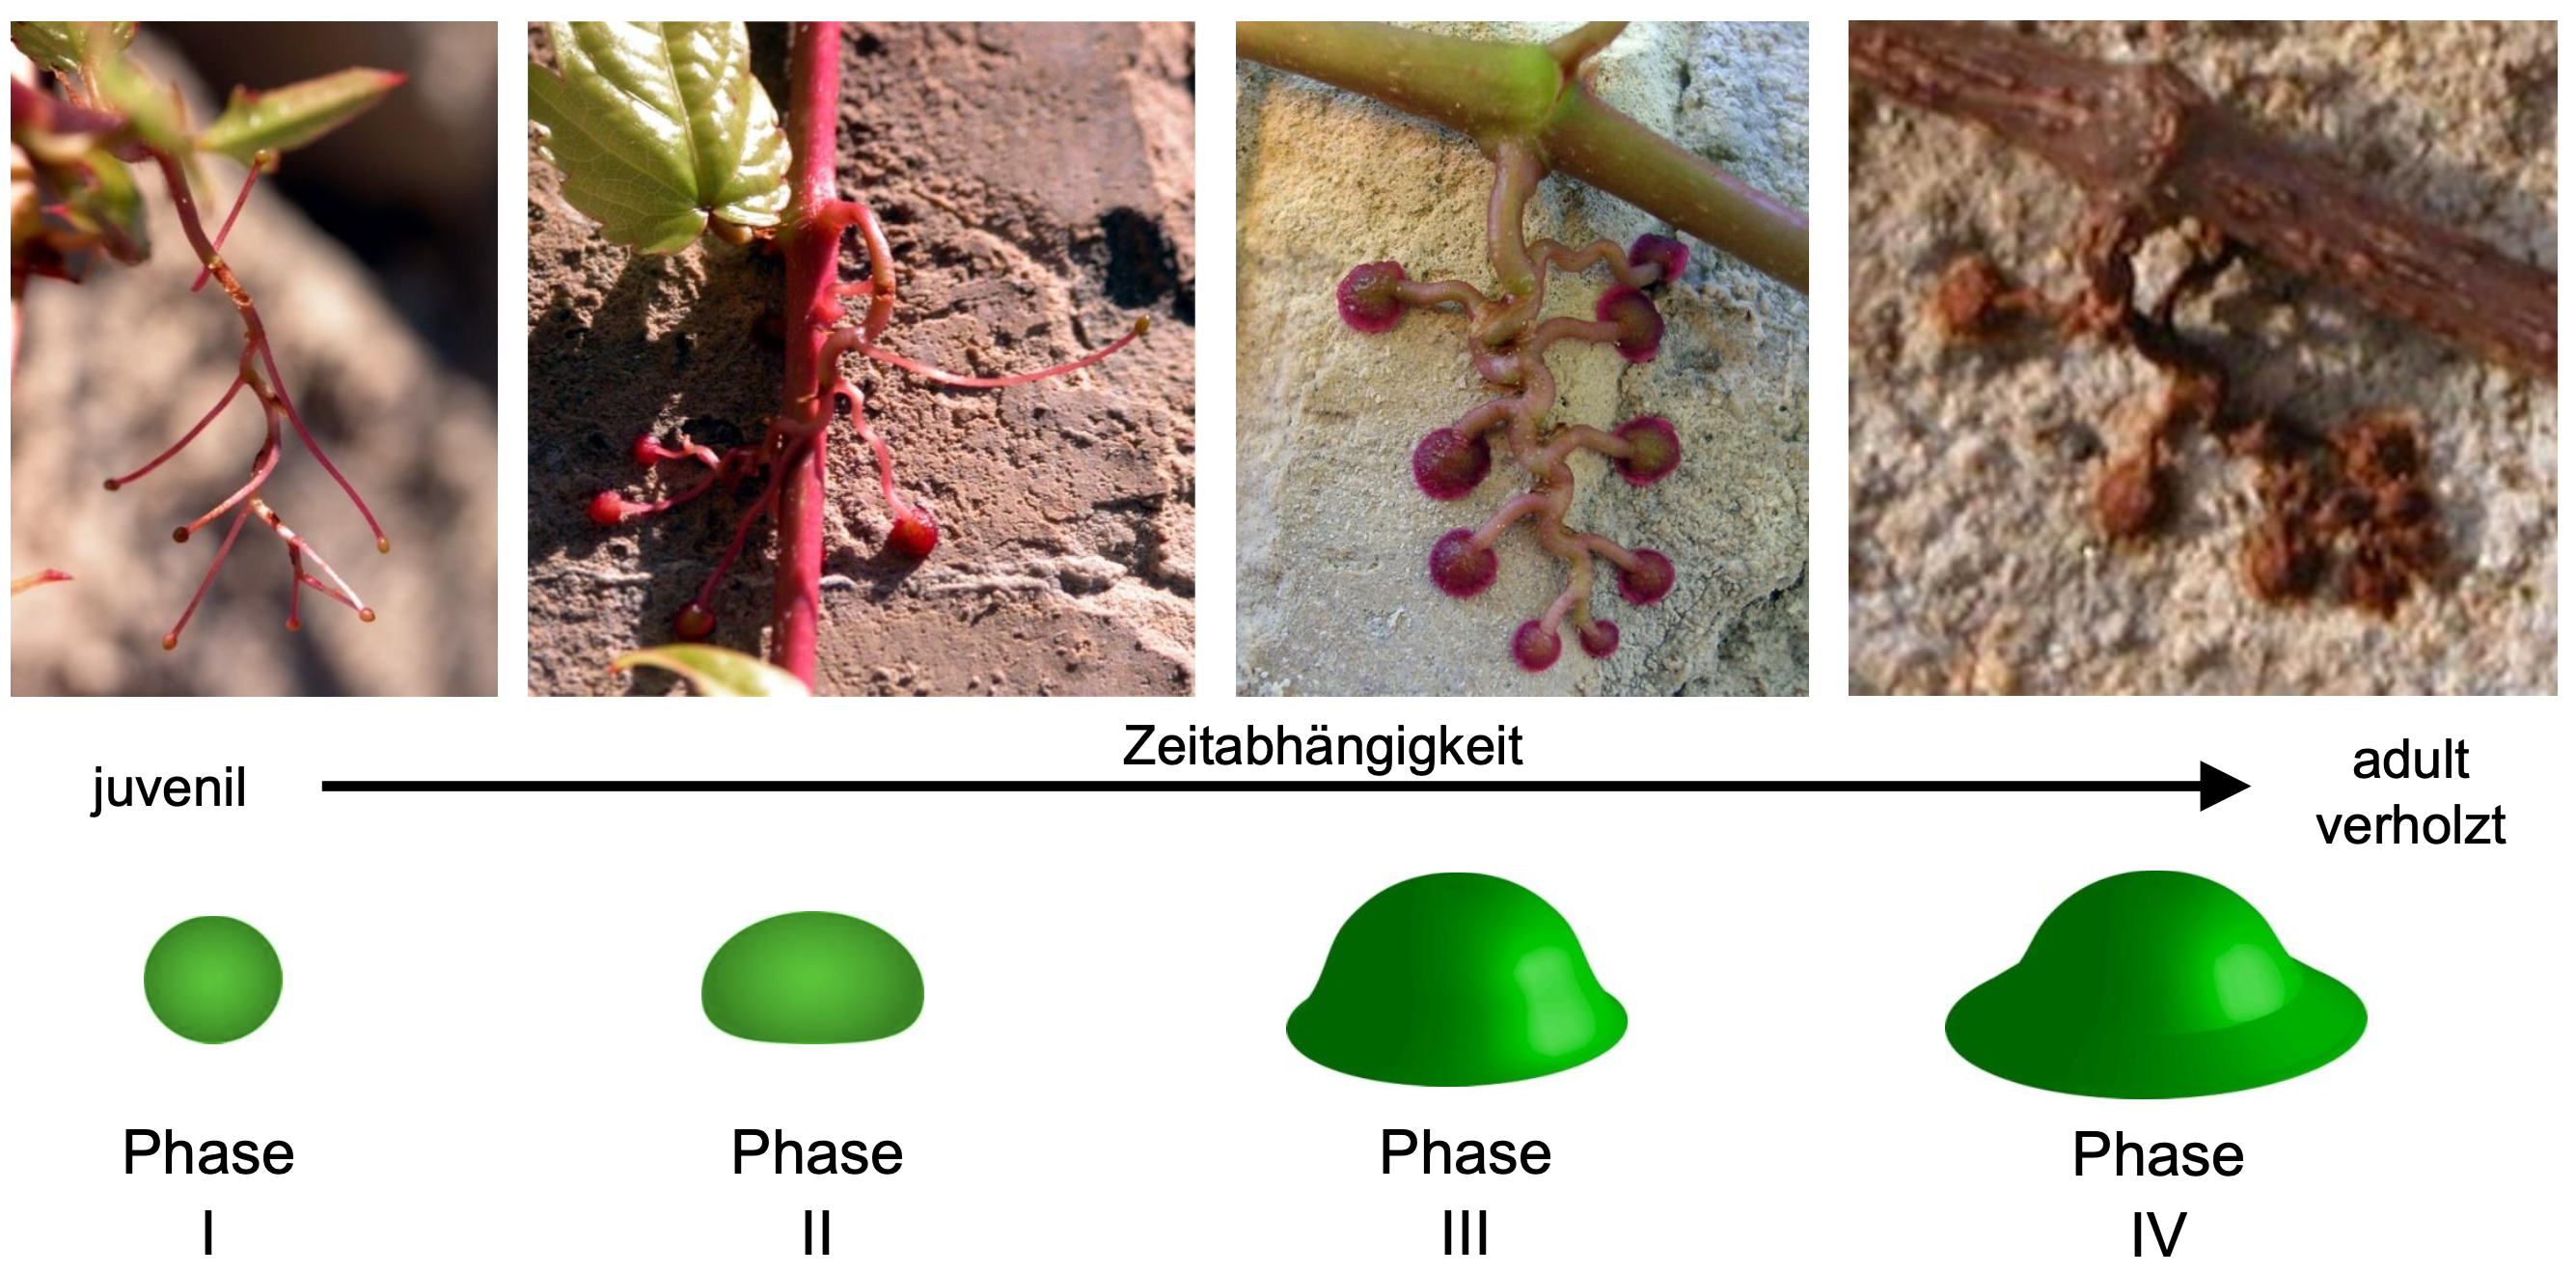
\includegraphics[width=9cm]{lec4/figures/wein_zeit.png}
    \hfill
    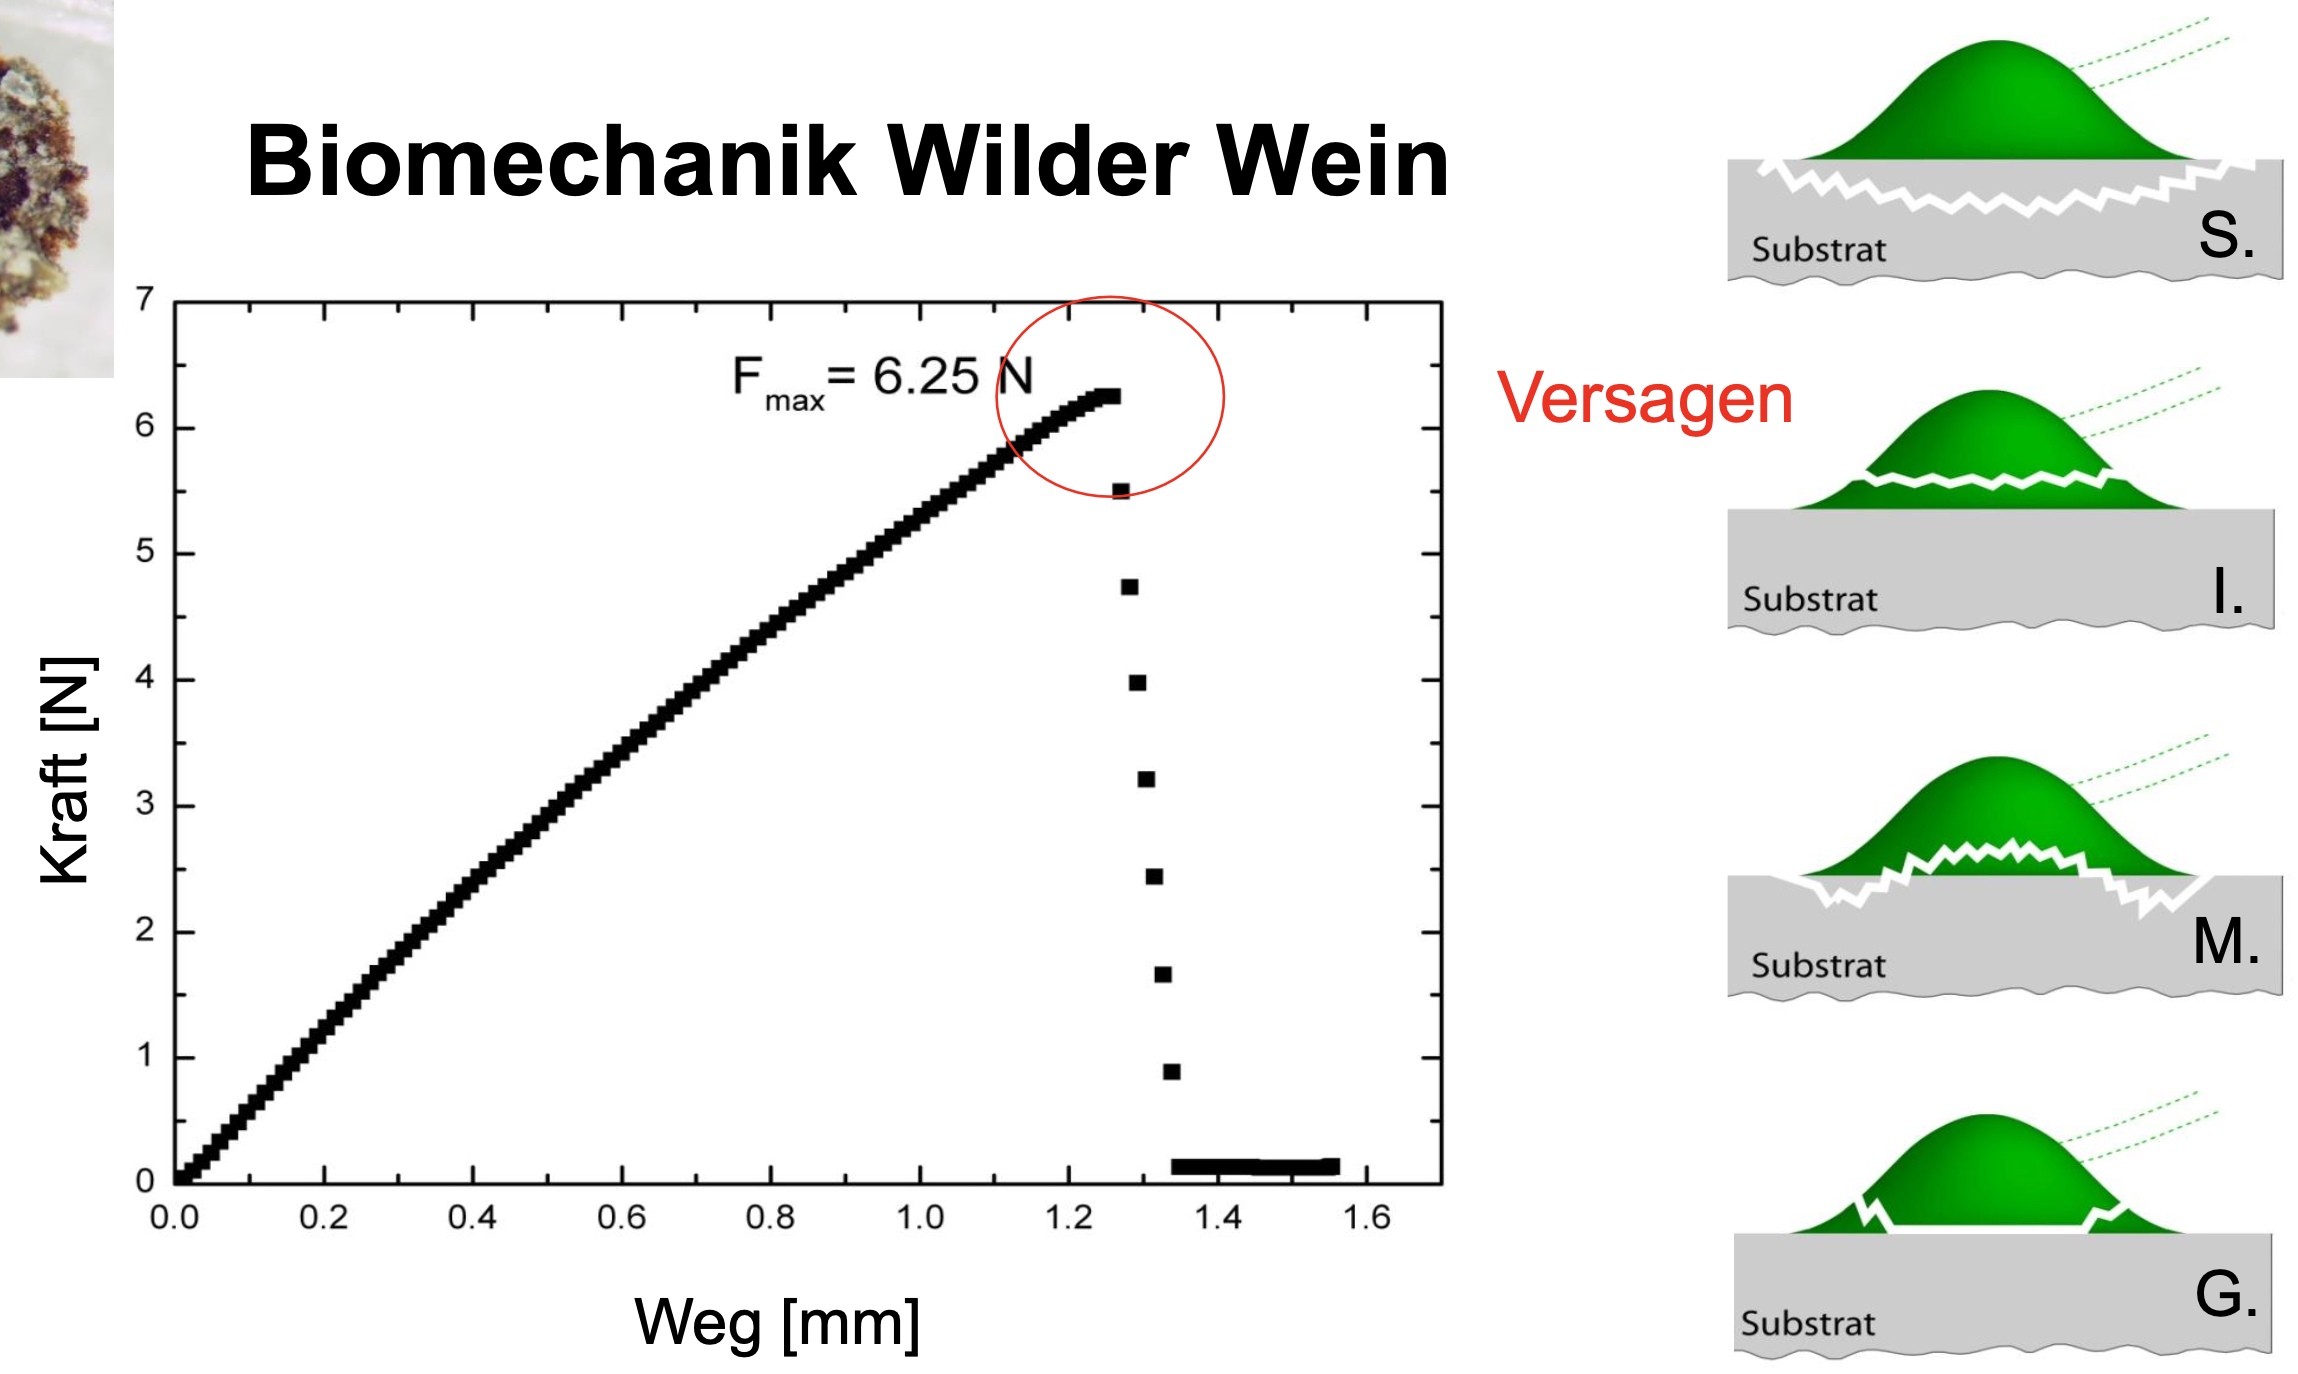
\includegraphics[width=7cm]{lec4/figures/wein_versagen.png}
\end{center}

\subsection{Technische Antihaftoberflächen nach dem Vorbild von „schlecht begehbaren“ Blattoberflächen}

\textbf{Beispiel 1:} Manche Blattoberflächen sind von Insekten schlecht begehbar. Im Versuch wird die Laufkraft von Insekten auf unterschiedlichen Oberflächen aufgenommen. Dabei zeigt sich, dass die geringe Laufkraft auf Blattoberflächen nicht dadurch ensteht, dass die Pflanzenkutikula die ``Härchen'' der Insekten verschmutzt. Stattdessen reduzieren Strukturen auf der Blattoberfläche die effektive Kontaktfläche auf der Haftkraft ausgeübt werden kann. Solche Strukturen verhindern entweder die Entstehung von Van-der-Waals Kräften (D im rechten Bild) oder das ``Einkrallen'' in die Oberfläche (E im rechten Bild).

Technische Umsetzungen: Antihaftfolien zur Schädlingsbekämpfung.

\begin{center}
    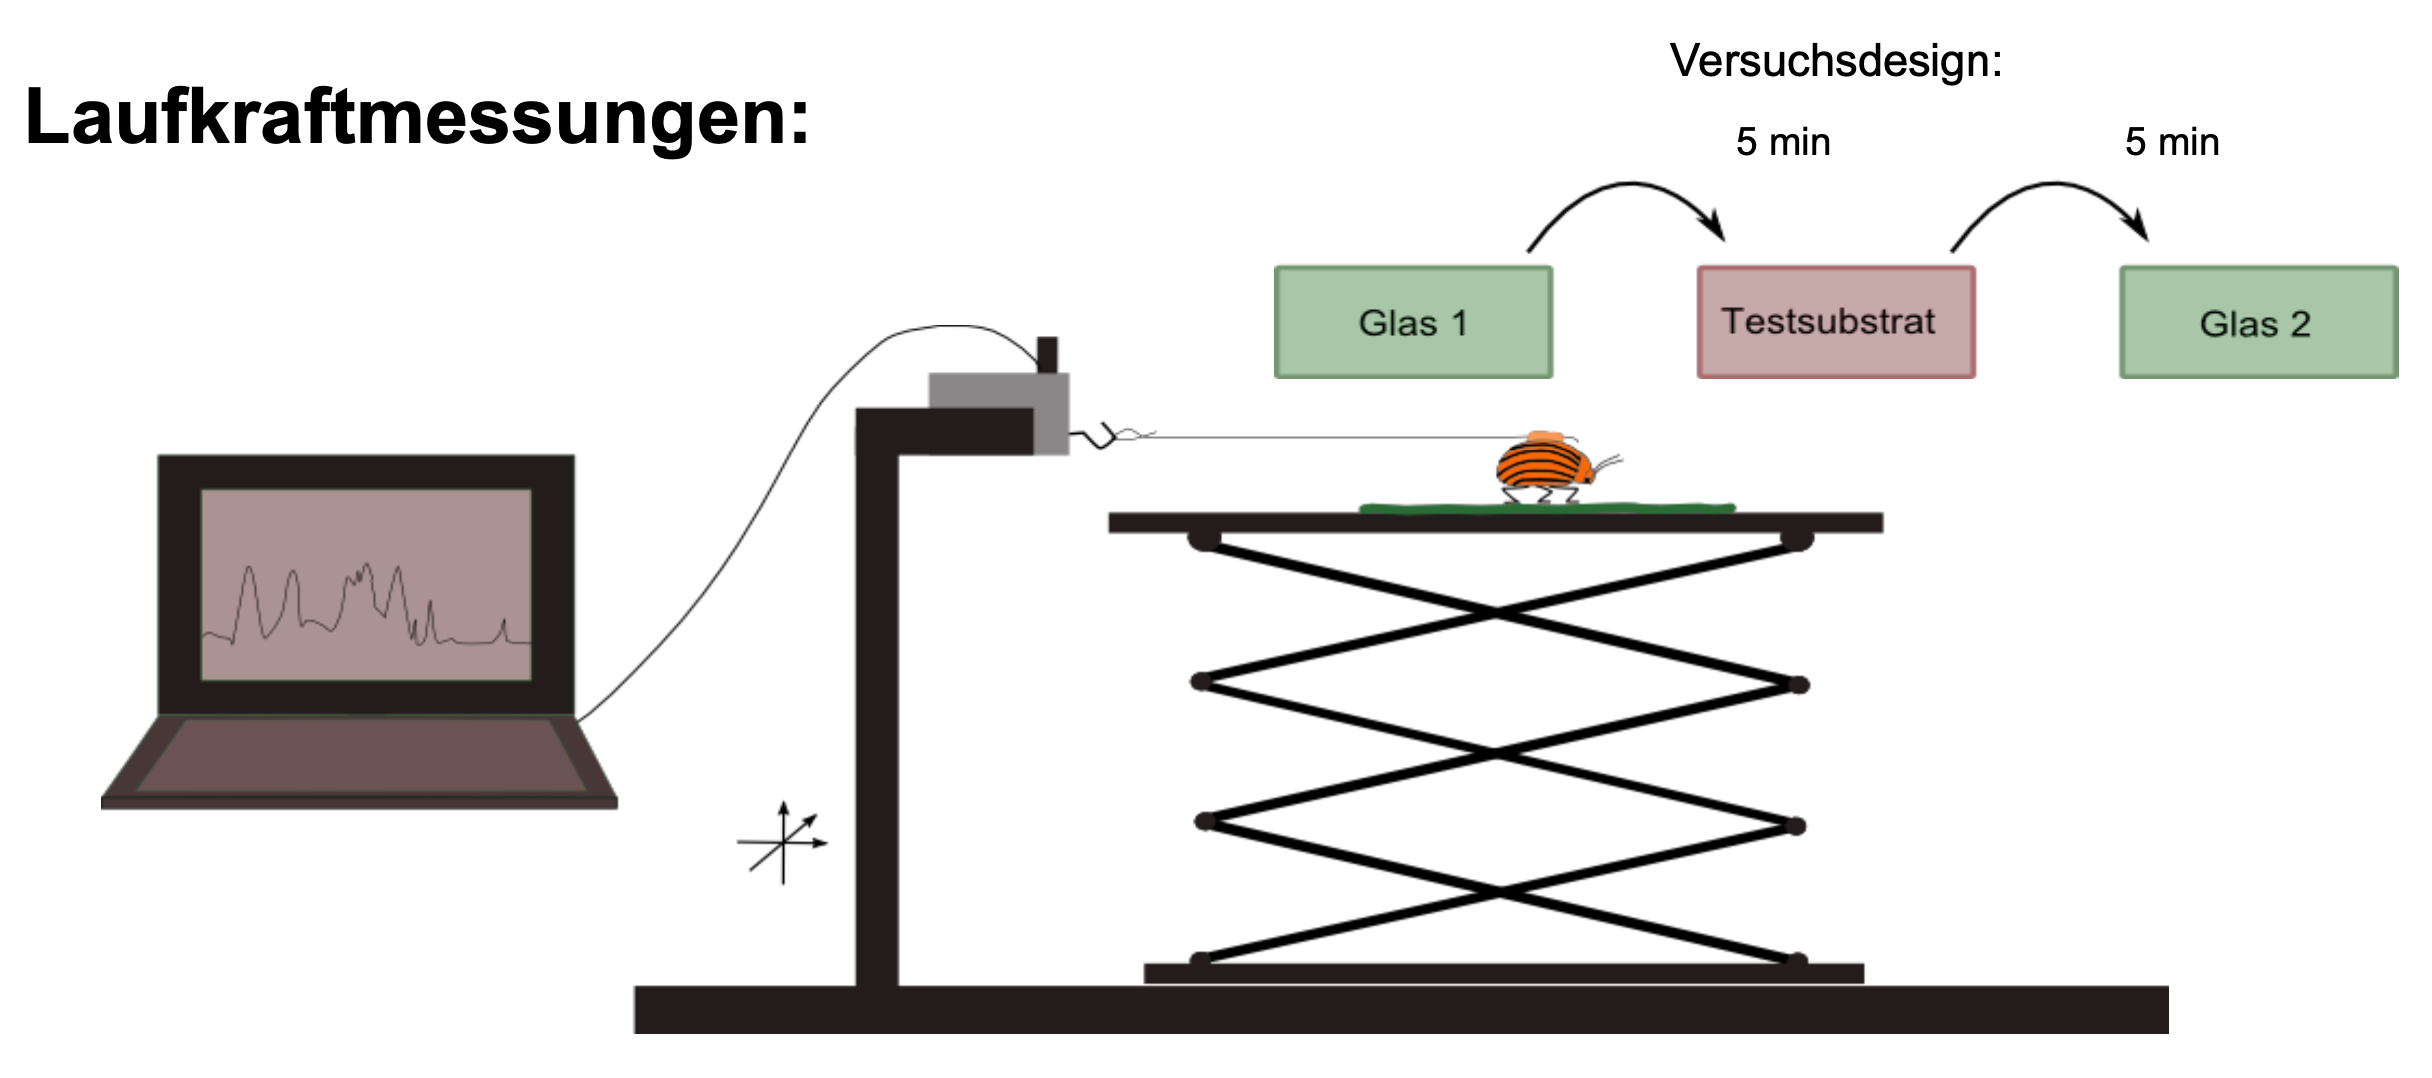
\includegraphics[width=12cm]{lec4/figures/laufkraftmessung.png}
    \hfill
    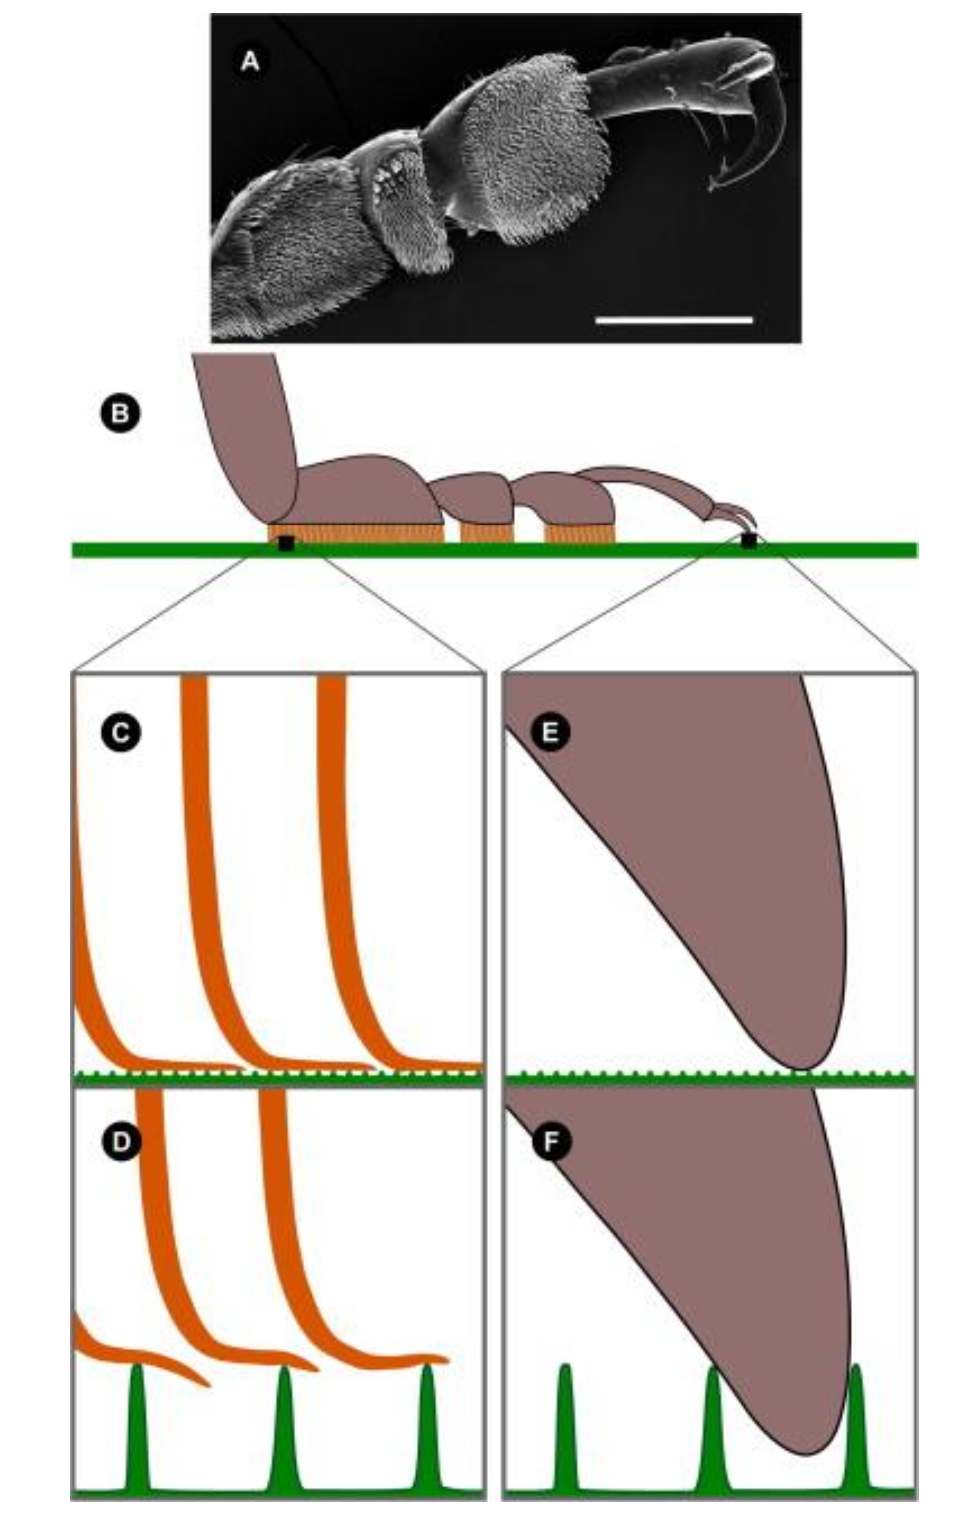
\includegraphics[width=4cm]{lec4/figures/blatt_haftung.png}
\end{center}
\textbf{Beispiel 2: Fleischfressende Pflanzen als Vorbild für Antihaft-Beschichtungen.} Ameisen rutschen an der inneren Wand ab. Die Oberfläche der Pflanze hat eine schwammartige Struktur und eine technische, ähnliche Funktions-Oberfläche (grün im Bild rechts) muss 3 Kriterien erfüllen \dangersign:
\begin{enumerate}
    \item Der Schmierfilm muss in das Substrat eindringen können
    \item Der strukturierte Festkörper muss vom Schmierstoff besser benetzt werden als von der abzuweisenden Flüssigkeit
    \item Die beiden Flüssigkeiten dürfen nicht miteinander mischbar sein $\rightarrow$ \textcolor{red}{Schmierfilmbildung}
\end{enumerate}
Ein Vorteil dieser Funktions-Oberfläche ist, dass sie \textit{auch bei Rissen abweisend} bleibt und aufgrund der Schmierflüssigkeit in der Struktur \textit{besser optisch durchlässig} ist als eine strukturierte Schicht ohne der Flüssigkeit.

\begin{center}
    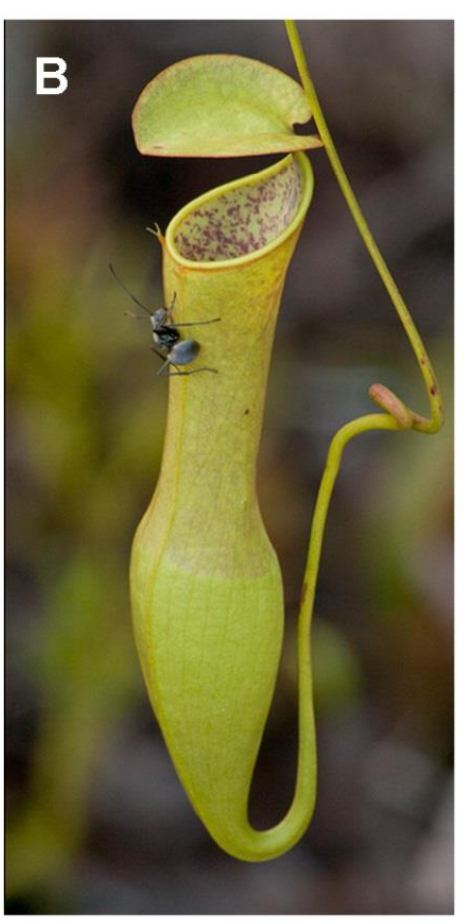
\includegraphics[width=2cm]{lec4/figures/ameise.png}
    \hfill
    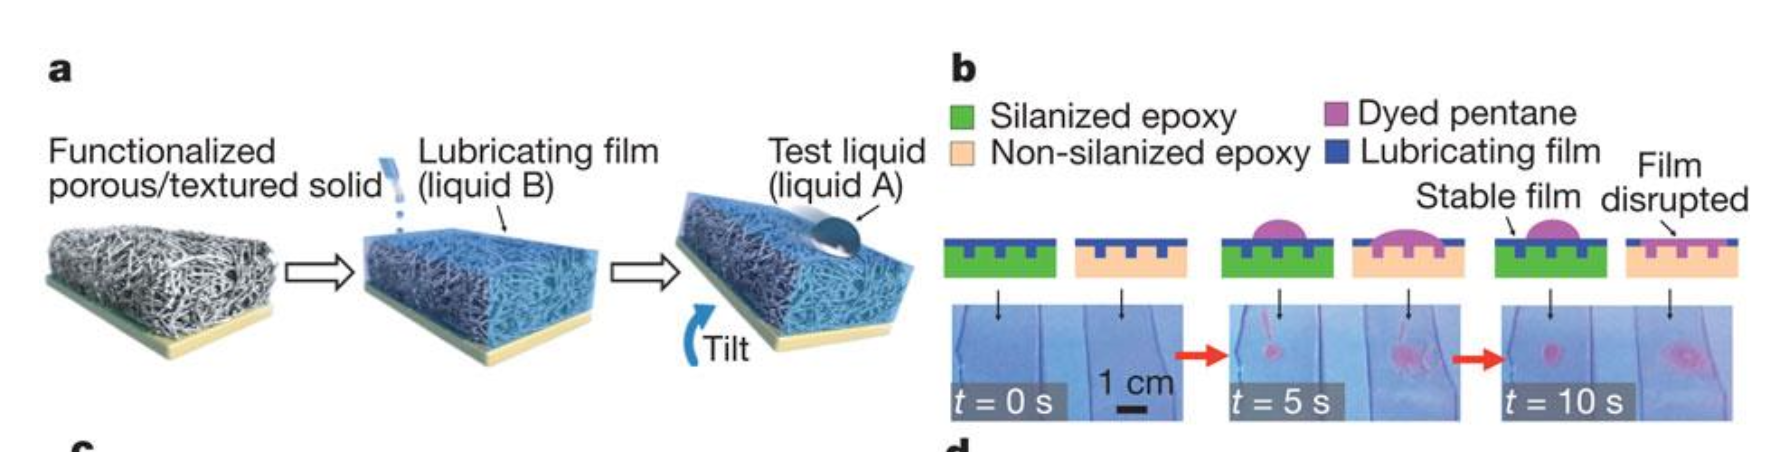
\includegraphics[width=14cm]{lec4/figures/slips.png}
\end{center}

\textit{Mögliche technische Anwendungen:} In der Medizintechnik aufgrund guter Antifouling Eigenschaften, da Bakterien nicht anhaften können (+ in der Schifffahrt). Dieser Antifouling Effekt wird allerdings nicht von der Oberfläche selbst hervorgerufen, sondern von einzer zusätzlichen aufgetragenen antibakteriellen Pflanzenschicht, welche sich in der schwammartigen Struktur einlagert. In Öl-pipelines, Optik, etc. Vorteile ggü.\ dem Lotus-Effekt sind \dangersign:

\begin{itemize}
    \item Fähigkeit auch Öle aubzuweisen
    \item Funktionieren auch unter hohem Umgebungsdruck
    \item Transparent
    \item Selbstreparatur
\end{itemize}
\section{Seblstreparatur in Biologie und Technik}

\subsection{Selbstreparatur in der Natur}

\textit{Wo findet man geeignete Lösungen von Selbstreparatur in der Natur?}

\begin{center}
    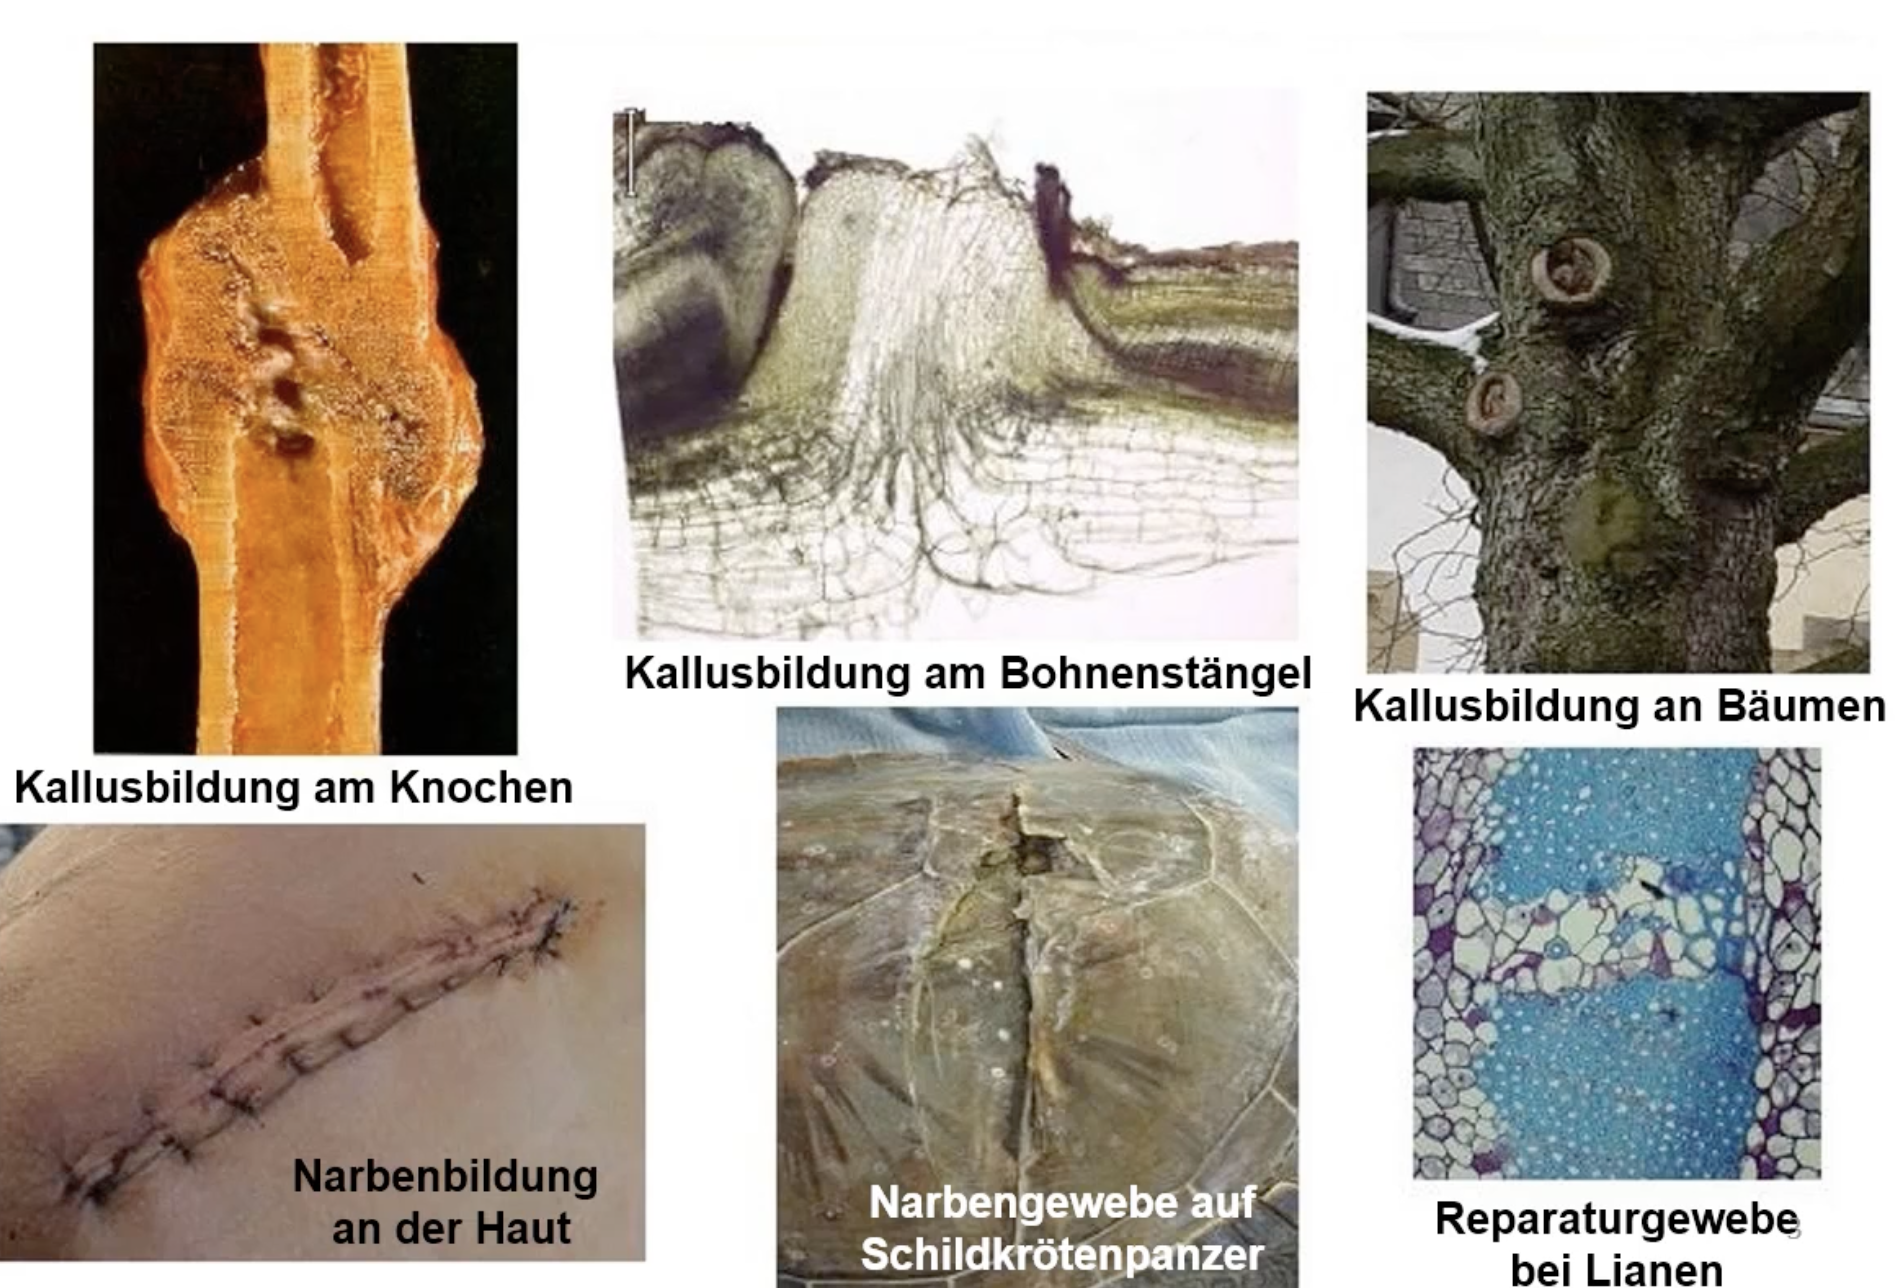
\includegraphics[width=12cm]{lec5/figures/selbstheilung-natur.png}
\end{center}

\begin{itemize}
    \item Kallusbildung am Knochen: Durch Zellwachstum werden die gebrochenen Teilstücke wieder zusammengeführt und sind danach stärker als zuvor (ein Knochen bricht niemals an derselben Stelle zweimal). \item Dadurch wird der Knochen allerdings schwerer.
\end{itemize}

\subsection{Selbstreparatur in der Technik}

\textit{Welche bestehenden Lösungen gibt es bereits in der Technik?}

\begin{center}
    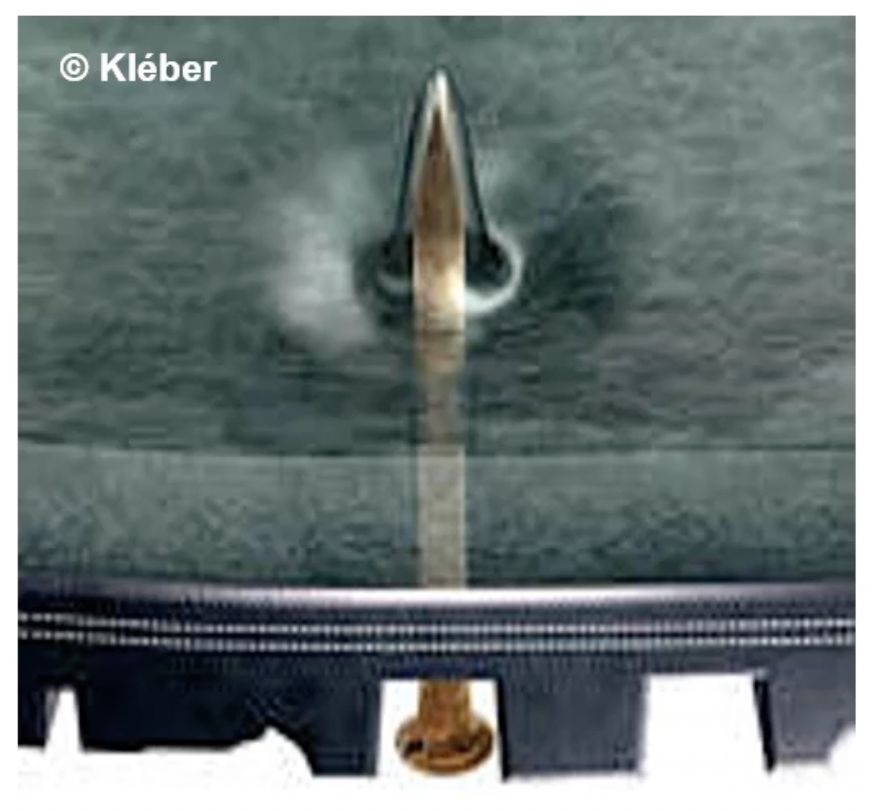
\includegraphics[width=5cm]{lec5/figures/selbstheilung-technik-1.png}
    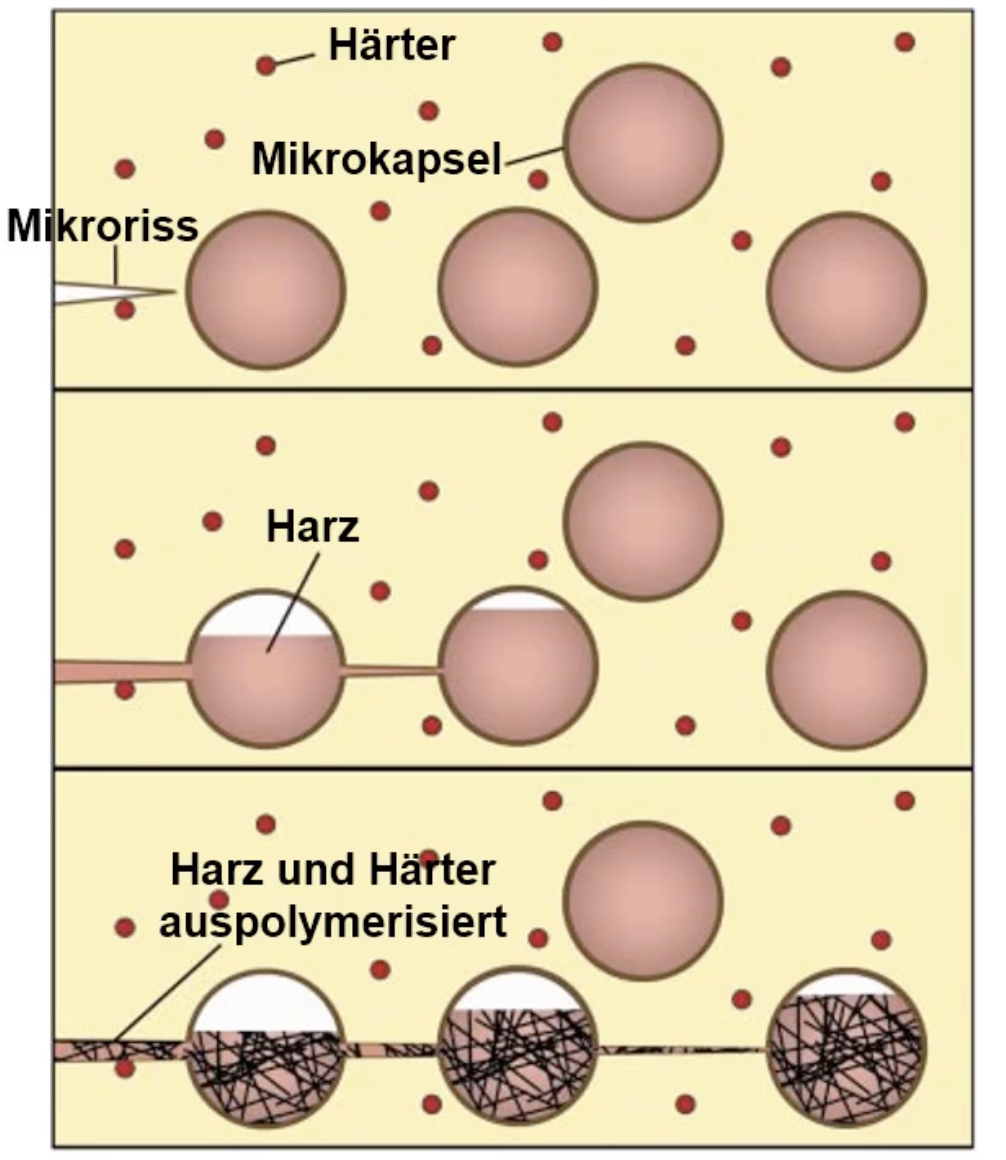
\includegraphics[width=5cm]{lec5/figures/selbstheilung-technik-3.png}
    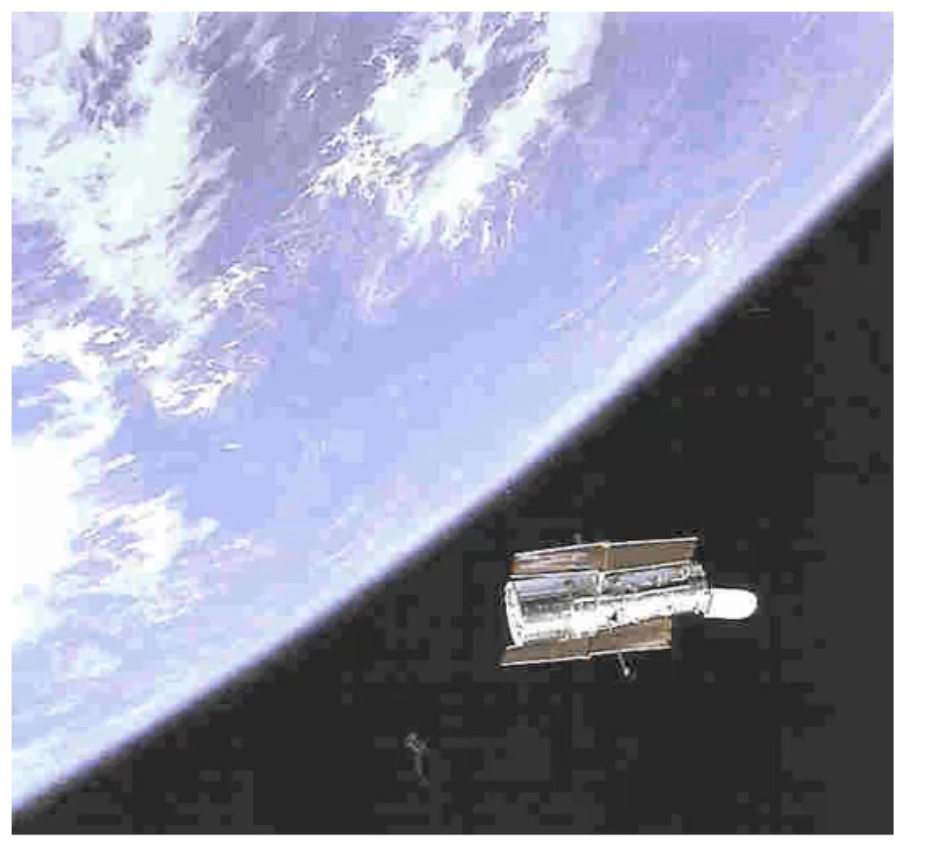
\includegraphics[width=5cm]{lec5/figures/selbstheilung-technik-4.png}
\end{center}

\begin{itemize}
    \item Reifendichtungsmittel (kein Bild): Kurzfristiger Reparatureffekt durch zähflüssige Emulsion mit synthetischen Fasern innerhabl des Reifens.
    \item \textbf{Selbstreparierender Autoreifen} (links): Bei punktartiger Verletzung der Struktur (bis 4,7 mm) zieht sich das Gewebe des Polymers aufgrund der Molekularstruktur zusammen und dichtet das Loch ab. 
    \item \textbf{Sebstreparierende spröde Polymere} (mitte): Struktur ist von Mikrokapseln mit Harz sowie kleinen Härterkügelchen durchsetzt. Werden beide angestochen und treffen aufeinander (durch Kappilareffekte), kommt es durch die 2-Komopenten-Wirkung zur Aushärtung.
    \item Organischer Beton (kein Bild): Beton, in welchen gefriergetrocknete Bakterien eingebracht werden, welche bei Eindringen von Fremdkörpern (z. B. Wasser) wachsen und Stoffe absondern, die den Beton "kitten".
    \item \textbf{Selbstreparierende Materialien für die Raumfahrt} (rechts): Verhinderung von Luftaustritt. Einziges bionisches Beispiel in dieser Auflistung, entwickelt nach Vorbild der menschlichen Blutgerinnung. Im Abschnitt ``Selbstreparatur in der Bionik'' beschrieben.
\end{itemize}

\subsubsection{Zweikomponentensysteme}

\textbf{Analyse der selbstreparierenden spröden Polymere}\\

\begin{center}
    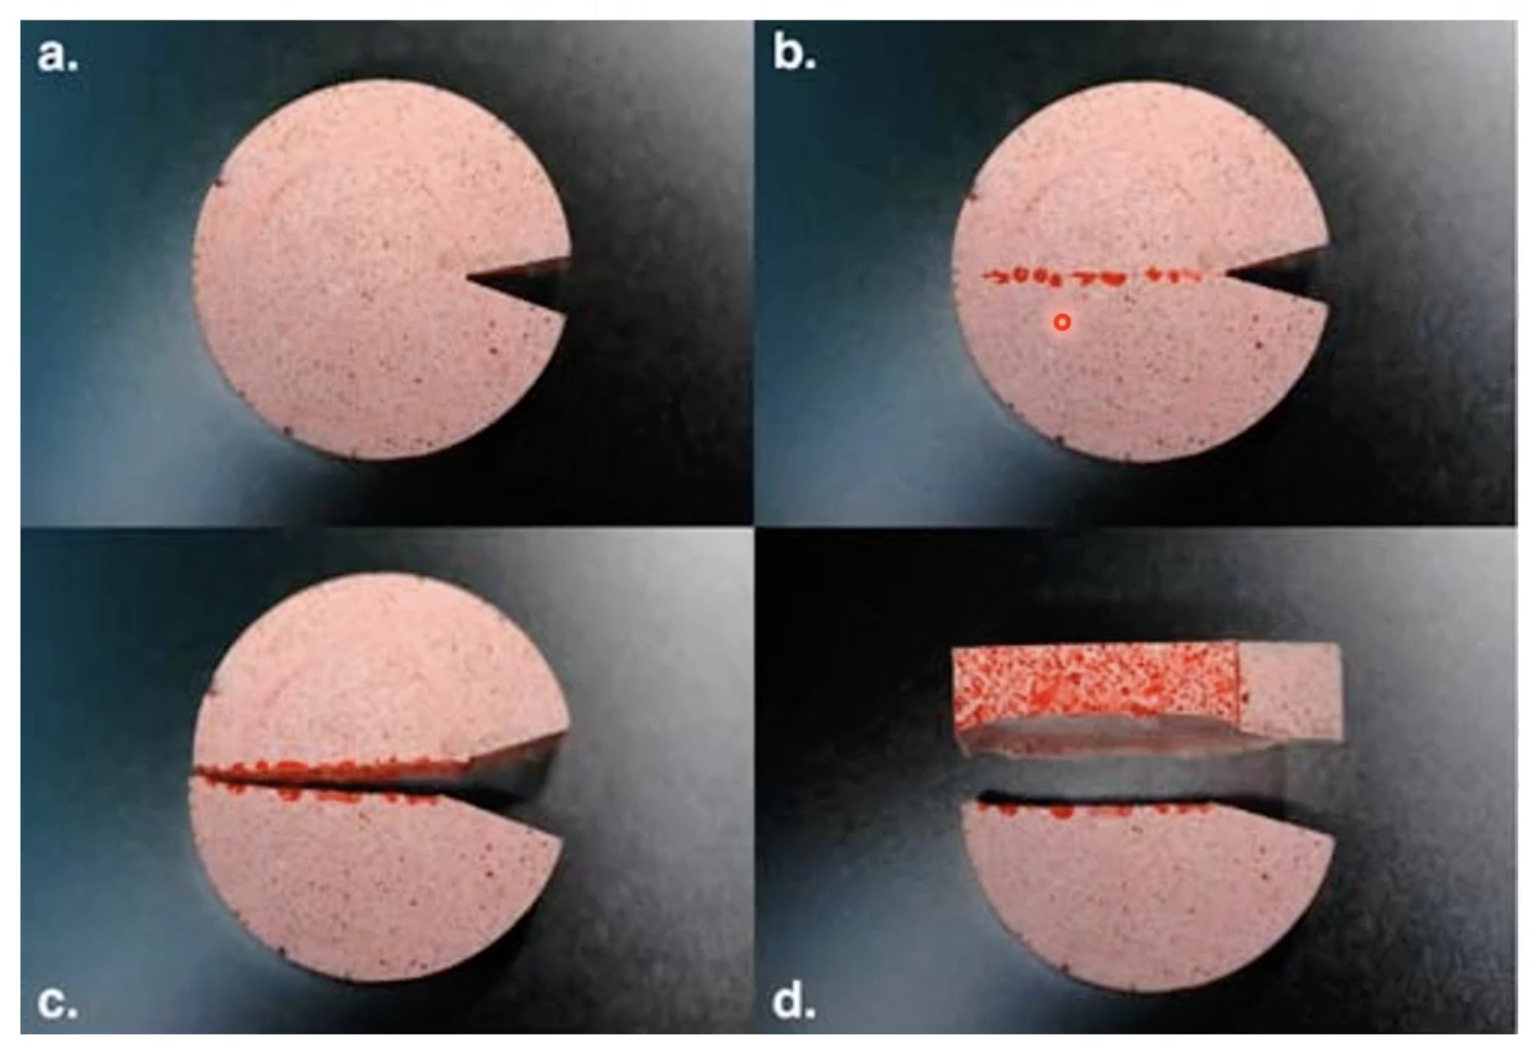
\includegraphics[width=7cm]{lec5/figures/selbstheilung-technik-2.png}
    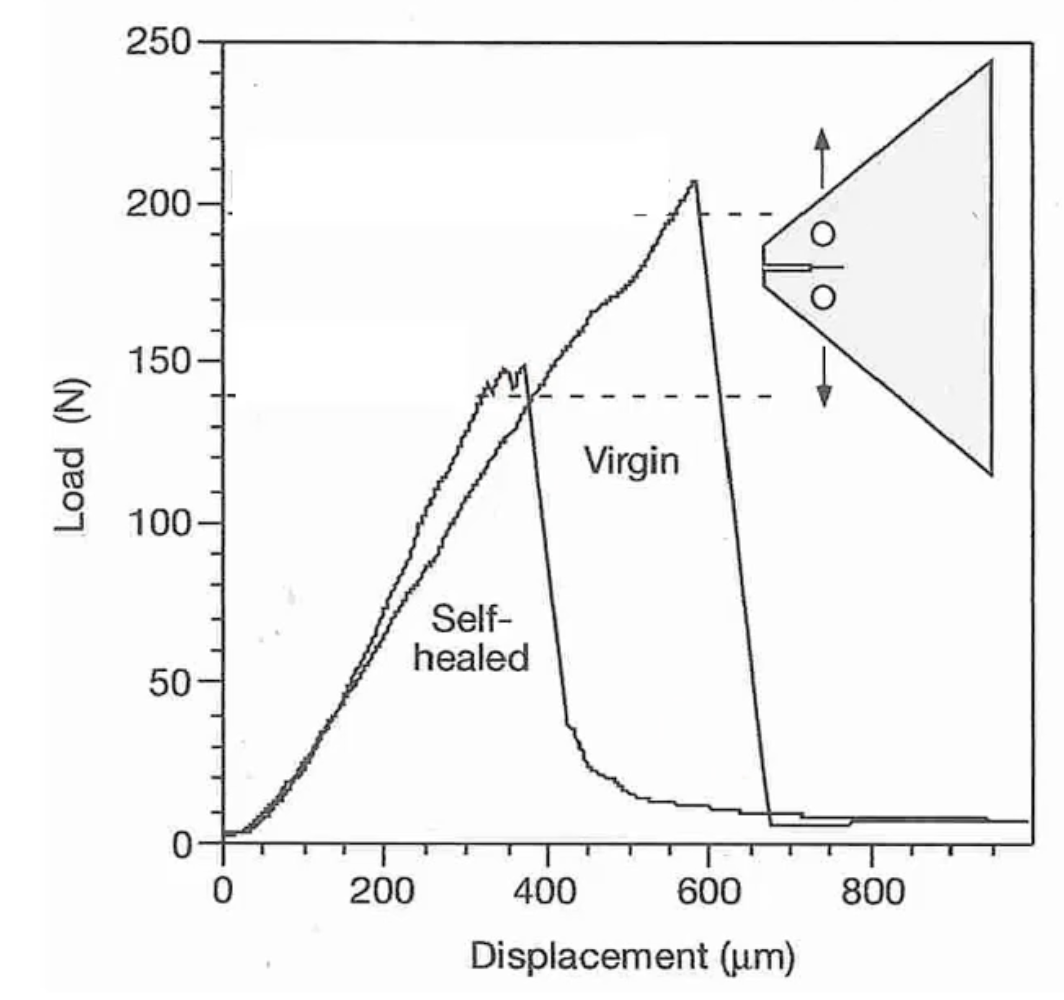
\includegraphics[width=6cm]{lec5/figures/zugversuch.png}
\end{center}

\begin{itemize}
    \item Optische Analyse mit REM, anhand derer der Kapillareffekt sichtbar sowie die Bruchstelle analysiert wird.
    \item Quantitfizierung anhand von Zugversuchen (siehe Kraft-Weg-Diagramm), 60\% der Bruchlast des selbstgeheilten Materials im Vergleich zum unbeschädigten Probenkörper.
\end{itemize}

\subsubsection{Quellende Hydrogele}

Neben den Zweikomponentensysteme mit zwei synthetischen Komponenten kommen auch Hydrogele (\textbf{SAP = superabsorbierende Polymere}) in den selbstreparierenden und -abdichtenden Materialien der Technik zum Einsatz, welche als zweite Komponente die Umgebungsfeuchte bzw. das Medium, gegen welches sie abdichten nutzen. Diese können enorm viel Feuchtigkeit aufnehmen und dadurch bis zur 1000-fachen Masse isotrop quellen. Sie kommen in Alltagsverbrauchsgütern z. B. bei Windeln, im technischen Einsatzgebiet bei Dichtungen zum Einsatz.\\

\begin{center}
    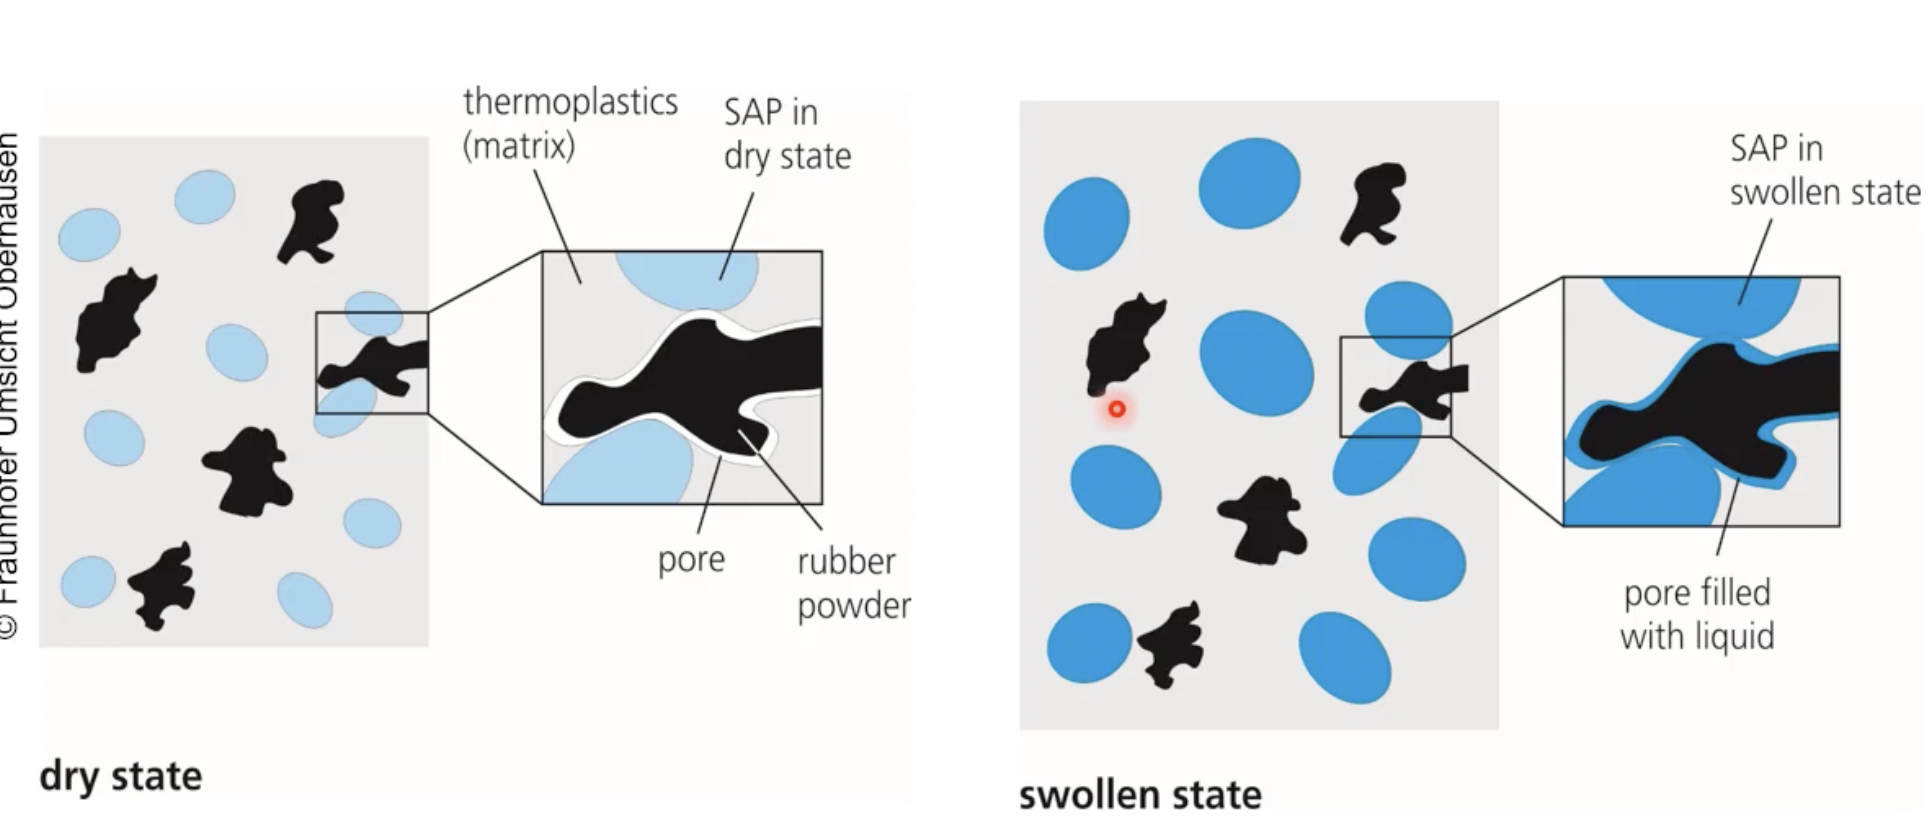
\includegraphics[width=14cm]{lec5/figures/TPE.png}
\end{center}

Diesen Effekt machen sich die \textbf{thermoplasitschen Elastomerkomposite} zu Nutzen, welche aus Gummipuder, SAP und Thermoplaste bestehen. Gummipuder und SAP sind dabei in eine Thermoplast-Matrix eingelassen (Bild). Sie haben ähnliche Eigenschaften wie Gummi, lassen sich ähnlich produzieren wie Thermoplaste (flexible Formgebung), quellen isotrop wie SAP und lassen sich hervorragend recyclen. Ein Anwendungsfall hierfür ist der Dichtschlauch Tangit.\\

Ein Nachteil quellfähiger Dichtungen ist, dass die Quellung nicht auf den Rissbereich beschränkt ist, wodurch die Formstabilität der Dichtung leidet. Dem wird vorgebeugt, indem die Dichtung durch einen speziellen Einbau von formstabilem Material umschlossen wird.

\subsection{Selbstreparatur in der Bionik}

\subsubsection{Abdichtung nach Vorbild der menschlichen Blutgerinnung}

Selbstreparierende Materialien in der Raumfahrt nach Vorbild der Blutgerinnung im menschlichen Körper.

\textbf{Blutgerinnung im menschlichen Körper.} (Nicht im Detail für die Klausur notw.)

\begin{enumerate}
    \item Fremdkörper oder Riss verletzt Integrität des Blutgefäßes.
    \item Blut tritt aus Blutbahn aus und kommt mit Gewebe in Kontakt.
    \item Sensorik in Haut registriert Blut und startet durch Gewebe- und Plasmafaktoren die Blutgerinnungskaskade.
    \item Enzyme werden kaskadenartig (und damit selbstverstärkend) produziert, welche wiederum neue Enzyme produzieren, bis Fibrin hervorgerufen wurde.
    \item Fibrinfasern vernetzen und bilden mit Thrombozyten und roten Blutkörperchen einen Thrombus, der die Wunde verschließt.
\end{enumerate}

\begin{center}
    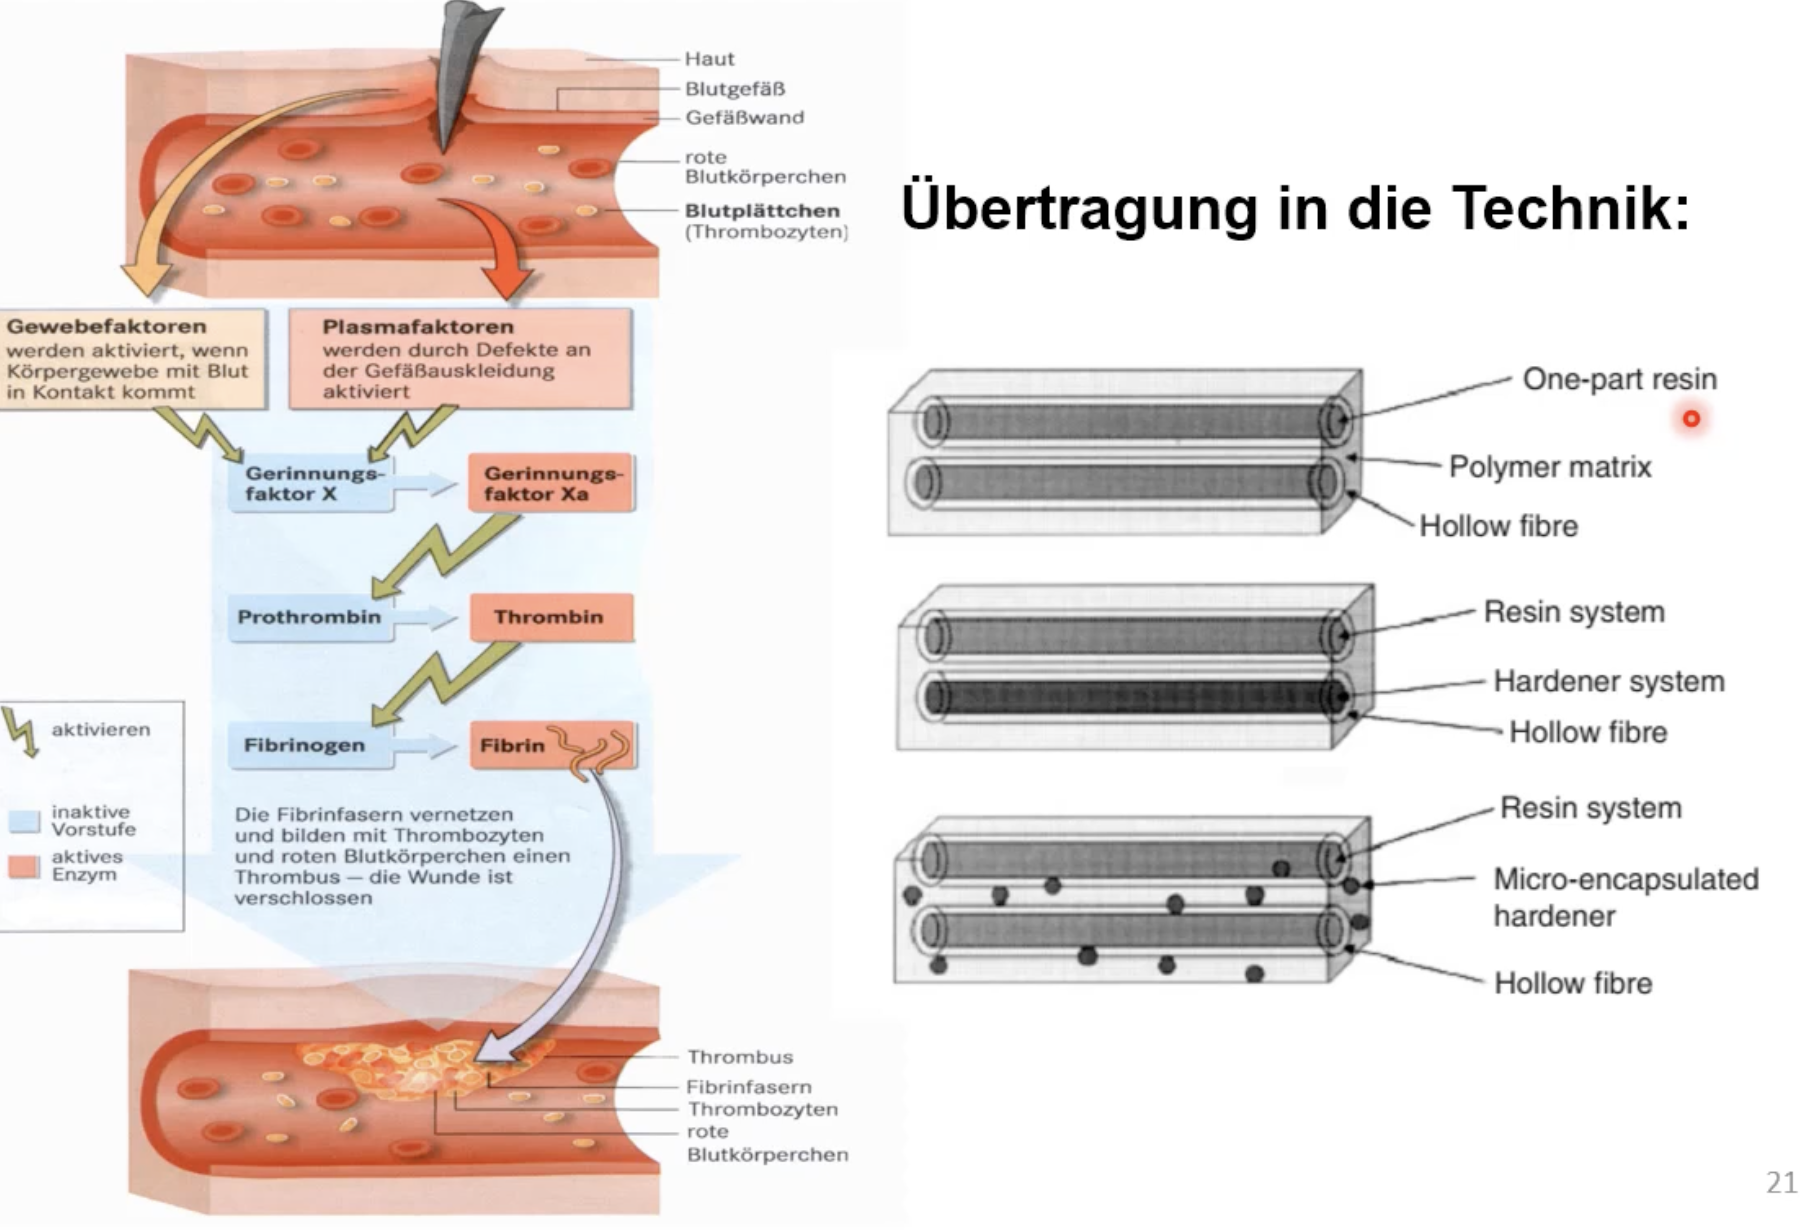
\includegraphics[width=14cm]{lec5/figures/blutgerinnung.png}
\end{center}

Ein Nachteil des Blutgerinnungsprozess ist es, dass nach Wundheilung die wieder abgelösten Fibrinfasern in \textbf{Engstellen des Blutkreislaufes} stekenbleiben können (z.B. durch Fett verkalkte Gefäße oder schmale Herzkranzgefäße). Durch Verstopfung kann kein Sauerstoff mehr zu den hintergeschalten Zellen geführt werden, was im Herzen zum Herzinfarkt, im Gehirn zum Schlaganfall und in den Gliedmaßen zur Thrombose führen kann.\\

Die Vielzahl an Kaskaden hat folgende Notwendigkeiten:

\begin{itemize}
    \item Verstärkung der Reaktion, da Enzyme schnell reaktiviert werden können. Ein Enzym aktiviert mehrere Zielproteine.
    \item Vermeidung von Fehlreaktionen.
\end{itemize}

Für die \textbf{bionische Abbildung des Blutgerinnungsprozesses im Rahmen der Raumfahrt} zur Vermeidung von Lufteintritt wurde ein Zweikomponentensystem genutzt, bestehend aus Hohlfasern mit Resin, Härter-Mikrokapseln, welche in den Zwischenräumen eingelagert sind, und Glasfasern (siehe Bild, rechts unten) \dangersign.
\\\\
\textbf{Zusammenfassung}:

\begin{itemize}
    \item Blutgerinnung als Vorbild für selbstheilenden Materialien in der Raumfahrt \dangersign
    \item Blutgerinnung funktioniert über Signalkaskade (Verstärkung + Vermeidung von Fehlreaktionen)
    \item Übertragung auf Technik durch 2-Komponenten Kunstharzsystem
    \item Kunstharz wird zusammen mit UV-Farbstoff in Hohlfaser gegeben
    \item Anordnung der Hohlfasern in Verbundmatrix mit Glasfasern
    \item Hohlfasern sind in 90° Winkel zu Glasfasern ausgerichtet
    \item Gezielte Schadensanalyse durch Biegetest
    \item Unbeschadetes selbstheilendes Material hat geringere Biegefestigkeit als Material ohne Selbstheilungsfunktion
    \item Biegefestigkeit ist nach Schadensereignis vollständig wieder hergestellt
    \item UV-Farbstoff ermöglicht visuelle Überprüfung des Materials auf Schäden
    \item Aushärten erfordert hohe Temperaturen und viel Zeit
\end{itemize}

\subsubsection{Abdichtung nach Vorbild des biochemischen Wundverschlusses bei Pflanzen}

Als Motivation für diese bionische Forschung dienen Polymere in Anwendungen mit hoher mechanischer Belastung, bei denen ein Versagen von Konstruktionen auftritt, bevor die eigentliche Beanspruchungsgrenze erreicht ist. Die \textbf{intrisisch aktivierte} Selbstreparatur nach Vorbild des biochemischen Wundverschlusses bei Pflanzen dient dazu, plötzlichem Versagen durch unkontrolliert wachsende Mikrorisse vorzubeugen \dangersign.\\

\textbf{Biologische Vorbilder} für dieses Vorgehen sind pflanzliche Sekrete und die für ihren Transport und ihre Speicherung zuständigen Gewebe und Zellen. 

\begin{itemize}
    \item \textbf{Sekrete} sind Milchsäfte (Ficus benjamina, Löwenzahn, Lotusblume, Schlafmohn, Würgefeige) und Harze (Kautschuk, Guttapercha, Gummi arabicum, Schellack als Ausscheidungen von Blattläusen, Balsam, Kiefern).
    \item \textbf{Transport- und Speichersysteme} sind Mikroröhren (Milchröhren, Harzgänge) oder spährische Harzbehälter/Mikrokapseln.
\end{itemize}
Baumharze härten aus, wenn die darin vorhanden \textbf{Turpentin-Öle} verdunsten. Durch die erneute Zugabe von Turpentin bzw. Terpentin kann der Harz wieder verflüssigt werden (Lösungsmittel).\\

\begin{center}
    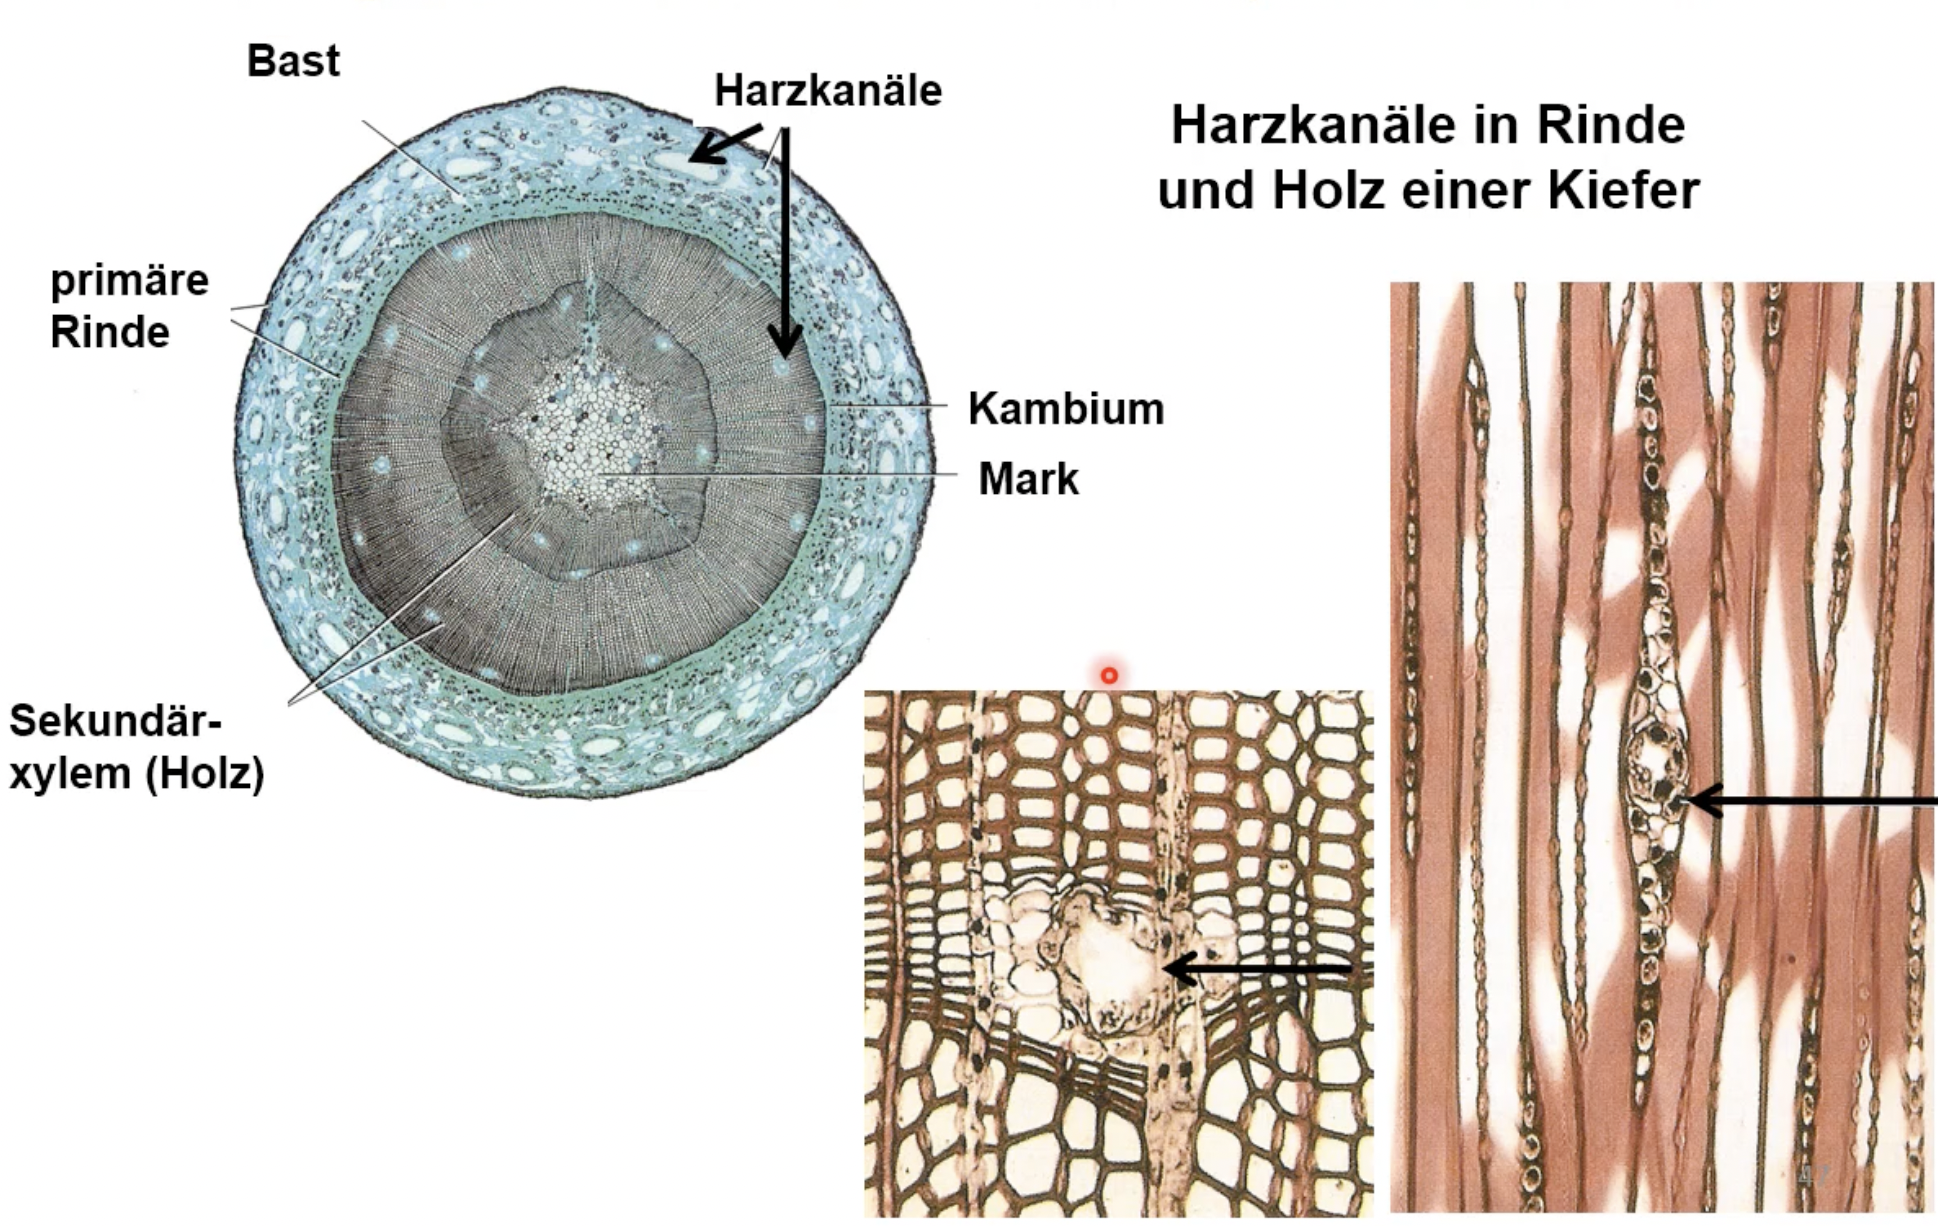
\includegraphics[width=11cm]{lec5/figures/baum.png}
    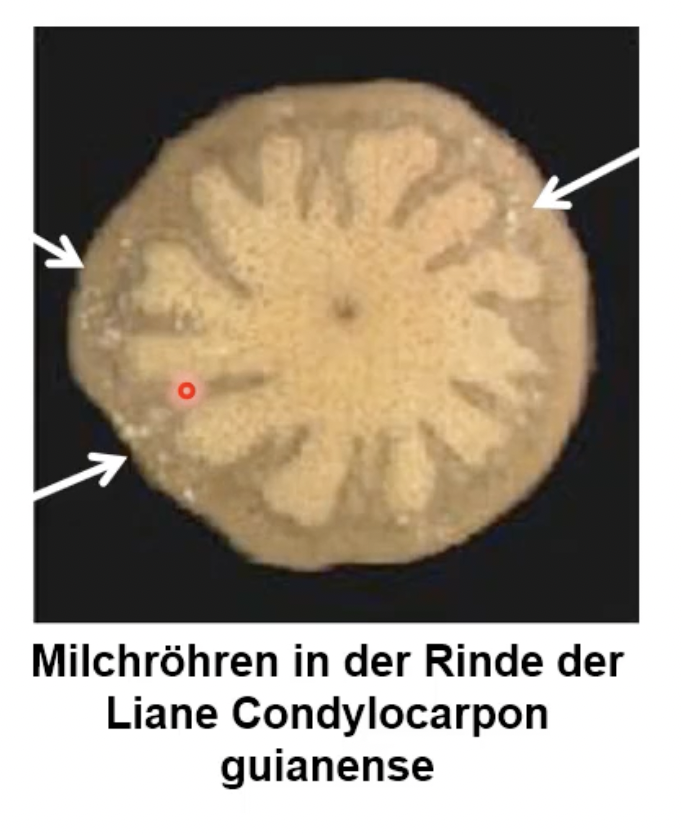
\includegraphics[width=5cm]{lec5/figures/liane.png}
\end{center}
Bei Bäumen wird ausschließlich im \textbf{Kambium} (Stammzellen der Bäume) Material gebildet (linkes Bild). Wenn das Kambium stirbt, stirbt auch der Baum. Nach innen wird Holz produziert, nach außen Bast. Dieser Wachstumsprozess ist deutlich unterschiedlich zu dem der Liane, bei der keine Trennschicht vorhanden ist (rechtes Bild).\\

\vspace*{2\baselineskip}

\textbf{Technische Umsetzung durch Mikrokapseln}\\

Eine Herausforderung der technischen Umsetzung ist es, Mikrokapseln herzustellen, welche mechanisch und thermisch stabil sind, materialgerechte chemische Selbstheilungseigenschaften haben sowie über ein geeignetes Wandmaterial verfügen. Der Stand der bionischen Forschung ist, dass man die Komponenten für die Selbstreparatur produzieren und bereitstellen kann, allerdings die funktionelle Biochemie des Seltsreparaturprozesses sowie die mechanischen Eigenschaften des reparierten Gewebes noch Optimierungsbedarf aufweisen.

\vspace*{2\baselineskip}

\textbf{Erforschung der biochemischen Prozesse der Selbstreparatur von Pflanzen}\\

Der bei Verletzung der Außenschicht austretende Milchsaft des Ficus Benjamina (Gartenfeige) trocknet innerhalb von wenigen Minuten aus und verschließt dadurch die Wunde. Untersuchungen haben Druckverhältnisse von über 8 bar im Inneren der Pflanze ergeben (vergleichbar mit Rennradreifen).\\

\begin{center}
    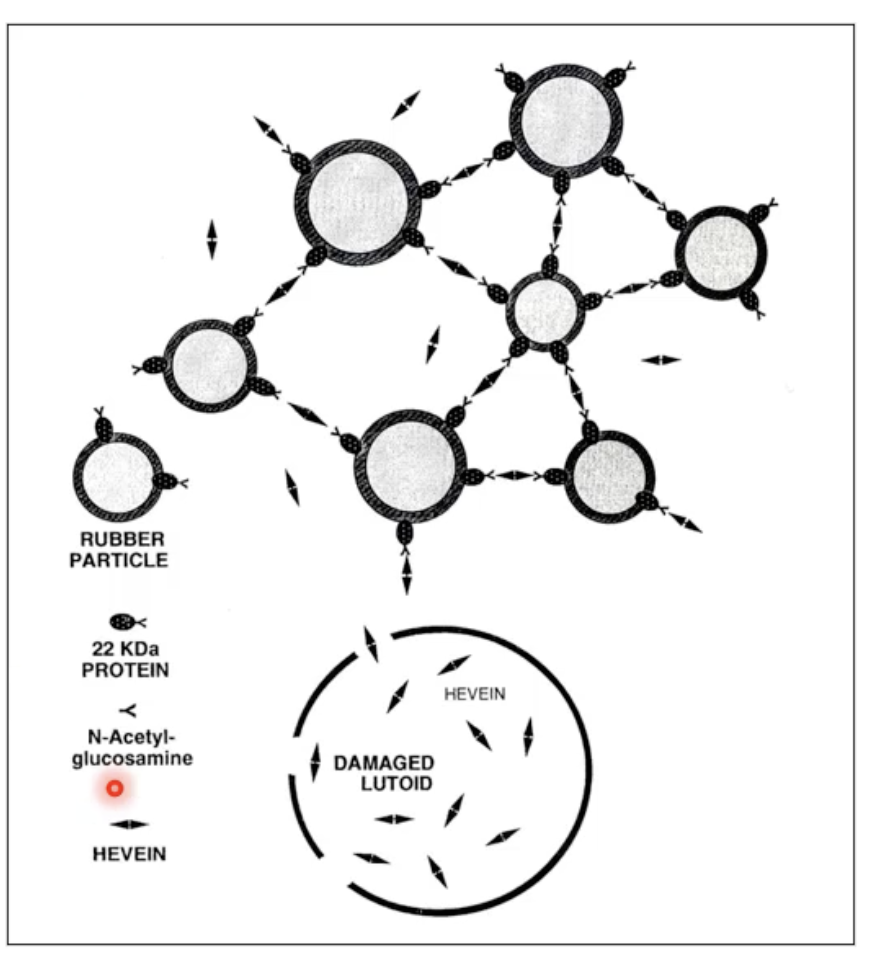
\includegraphics[width=8cm]{lec5/figures/milchsaft.png}
\end{center}
Der \textbf{Milchsaft des Kautschuk-Baumes (Latex)} ist eine Kolloidsuspension von negativ geladenen Latexpartikeln und \textbf{Lutoids} (membranumschlossene Vesikel). Sie befinden sich in Milchröhren (8 bar), im äußeren Bereich des Stammquerschnitts. Die \textbf{Koagulation} des Milchsafts tritt auf, da es durch den \textbf{Druckabfall}, welcher infolge eines Risses in der Außenhülle hervorgerufen wird, zu einem Aufplatzen der Lutoide kommt. Die darin enthaltenen \textbf{Hevein-Proteine} lagern sich an Bindestellen von im Milchsaft vorhandenen Gummipartikeln an und bilden so eine quervernetzte Kettenstruktur \dangersign.\\

\begin{center}
    \includegraphics[width=7cm]{lec5/figures/partikel-frisch.png}
    \includegraphics[width=7cm]{lec5/figures/partikel-wasser.png}
\end{center}
Die Koagulation ist pH-abhängig, das Optimum liegt bei einem pH-Wert von 5.5. Dadurch lässt sich mithilfe von Ammoniak die Aushärtung von eingelagertem Natur-Latex (Kautschuk) verhindern. Dieser Effekt ist in den oberen Grafiken für den Milchsaft des Ficus Benjamina zu erkennen und kann auch mithilfe von Tg-IR-Spektrokopie nachgewiesen werden.

\vspace*{2\baselineskip}

\textbf{Erforschung der mechanischen Eigenschaften der Reparaturmaterialien und reparierten Gewebe}\\

Die Tests zur Bestimmung der mechanischen Eigenschaften umfassen:

\begin{itemize}
    \item Zugfestigkeit, E-Modul, vollständige Spannungs-Dehnungsdiagramme mittels Mikro-Zugbühne
    \item Indentationstests auf Mikro- und Nanoebene mittels Mikro-Drucktester und Raster-Kraft-Mikroskop 
\end{itemize}

\begin{center}
    \includegraphics[width=10cm]{lec5/figures/sd.png}
\end{center}
Eine frisch verletzte Probe hat einen deutlich kürzeren Bereich der plastischen Dehnung und damit ein Totalversagen, welches schon bei ca. 25\% der maximalen Dehnung im Vergleich zur unverletzten Probe auftritt. Die Probe mit ausgeheiltem Riss verhält sich ähnlich, kann allerdings in diesem unteren Dehnungsbereich mehr Zugspannung als die unverletzte Probe aushalten. Die \textbf{Reparaturzeit} umfasst dabei bei den meisten Pflanzen ein Minimum von \textbf{10 min}. Da dies für viele technische Anwendungen zu lange ist, wurde ein spezielles Augenmerk auf die \textbf{Glockenblume} gelegt, welche bereits nach \textbf{2 s} signifikante Reparatureffekte aufweist \dangersign.

\vspace*{2\baselineskip}

\subsubsection{Abdichtung nach Vorbild des mechanischen Wundverschlusses bei Pflanzen}

Zugrundeliegendes Problem aus den Ingenieurswissenschaften sind pneumatische Strukturen, welche gegen Luftverlust abgedichtet werden müssen.

\begin{center}
    \includegraphics[width=14cm]{lec5/figures/top-down.png}
\end{center}
Motivation für die Erforschung der biochemischen Selbstreparturmechanismen bei Pflanzen ist die Vermeidung eines Luftverlustes bei Beschädigung der Außenhülle von pneumatischen Systemen. Ein relevanter Anwendungsfall hierfür ist die mobile pneumatische Brücke Tensairity (8m Spannweite, 3.5t max.\ Traglast).\\

Als \textbf{biologische Vorbilder wurden schnellwachsende Pflanzen wie bspw.\ die Liane oder der Bohnenstängel} betrachtet. Beim Rissverschluss wird kein neues Material aufgebaut, sondern das bestehende Material verteilt (Änderung der Zellform, Abnahme der Zellwanddicke, gleichbleibendes Zellwandvolumen). Verholzung erfolgt, allerdings auch erst nach mehreren Tagen. Durch Vierpunktbiegung wurde nachgewiesen, dass bei einer Verletzung quer zur Hauptrichtung des Bohnenstängels es erst zu einer signifikanten Abnahme des Biegeelastizitätsmoduls kommt (-40\% nach Tag 3), bis nach 15 Tagen die mechanischen Eigenschaften vollständig wiederhergestellt sind.\\

Abstraktion daraus ist ein technisches Modell mit \textbf{innerer Schaumschicht} aus unter Druck stehenden Zellen (bionische Umsetzung der Selbstreparatur bei Pflanzen) und einer \textbf{äußeren faserverstärkten Membran} der pneumatischen Struktur, wie in der folgenden Abbildung gezeigt. Verschiedene Schaumstrukturen in Zerstörungsprüfungen wurden untersucht. Beschichtung der Membran führt zu einem Reparaturfaktor von 12 (Dauer für Druckabfall 12-mal länger als bei unbeschichteter Membran). Ein \textbf{Überdruck während der Polymerisation} von 2 bar verbessert den Reparaturfaktor auf bis zu 1600.
\\\\
(\dangersign \textit{Worauf basiert die Selbstreparatur bei der Tensairity Luftkissenbrücke? Wie wird ein hoher Reparaturfaktor erreicht?})
\\\\
(\dangersign \textit{Nenne Beispiele für biologische Selbstreparatur + die technische Anwendung})


\begin{center}
    \includegraphics[width=11cm]{lec5/figures/funktionsmodell.png}
\end{center}

\subsubsection{Selbstschärfende Messer nach Vorbild von Nagetierzähnen}

\begin{center}
    \includegraphics[width=9cm]{lec5/figures/zahn.png}
    \includegraphics[width=5cm]{lec5/figures/messer.png}
\end{center}
Nagetierzähne wachsen 2-3 mm pro Woche, bleiben allerdings durch einen unterschiedlich starken Abrieb von weicher Spanfläche (Dentin) und harter Freifläche (Schmelz) sowohl in der Länge konstant als auch gleichermaßen an der Zahnspitze scharf. \\

Messer, welche beim Schneiden durch harte Partikel im zu schneidenen Material abstumpfen, müssen zeitaufwändig geschnitten werden. Nach Vorbild des Nagetierzahns wurden daraus selbstschärfende Messer für Industrieschneidemaschinen entwickelt. Ein Nachteil ist, dass immer harte Materialien geschnitten werden müssen um den Effekt der Selbstschärfung auferechtzuerhalten.
\section{Selbstorganisation und Verpackungen}

Organismen organisieren sich in hierarchischen Ebenen: Molekül $\rightarrow$ Organell $\rightarrow$ Zelle $\rightarrow$ Gewebe $\rightarrow$ Organ $\rightarrow$ Lebenwesen $\rightarrow$ Ökosystem.
\\\\
\textbf{Was ist Selbstorganisation \dangersign?} \textcolor{red}{Spontane Strukturbildung in nicht linearen dynamischen Systemen}. Durch Selbstorganisation entstehen zeitlich, räumlich oder funktional geordnete Strukturen. \textit{Biologische Strukturen basieren auf Hierarchien sowie Grenz- und Oberflächen auf allen Größenbereichen.}

\subsection{Organisationsebenen von Organismen}

\textbf{Bspl.\ bei biologischen (auf Molekülebene):} Bei geeigneten Umweltbedingungen, spontan aufgrund der Moleküleigenschaften (d.h. ohne Einwirkung äußerer Faktoren) erfolgende Bildung komplexer Strukturen bei: Makromolekülen, Membranen, Zellen, Zellverbänden... $\rightarrow$ Phospholipide bilden z.B.\ in Wasser eine Micelle oder Doppelschicht. Dieses Phänomen tritt bei Zellwänden auf.

\begin{center}
    \includegraphics[width=5cm]{lec6/figures/phospholipid.png}
    \hfill
    \includegraphics[width=10cm]{lec6/figures/zellwand.png}
\end{center}
\textbf{Bspl.\ Schwarmverhalten} von Vögeln/Fischen. Dient dem Schutz vor Jägern.
\\\\
\textbf{Bspl.\ Ameisenalgorithmus:} Wie wird der kürzeste Weg zwischen Nest (N) und Futterquelle (F) gefunden? Späherameisen finden Futterquellen zu Beginn auf zufälligen Wegen und hinterlassen dabei eine Pheromonspur. Weitere Ameisen folgen den Spuren zum Futter und hinterlassen selbst Pheromone. Da die Pheromone mit der Zeit verdunsten sind die Pheromonspuren auf kürzeren Spuren stärker als auf Längeren (da pro Zeit mehr Ameisen strömen) $\rightarrow$ Lösung wird optimiert ist aber nicht optimal. Nachteil: die optimale Lösung wird nie gefunden, wenn die Späherameisen nicht per Zufall auf sie stoßen. (Aus dem Internet: Ein Vorteil ist, dass als heuristischer Algorithmus schneller eine gute Lösung gefunden wird, als z.B.\ mit Breitensuche.)\\
\textit{Technische Anwendung:} Routing von Internetpaketen, Logistik, etc.
\\\\
(\dangersign \textit{Beschreibe den Ameisenalgorithmus + seine Vor- \& Nachteile.})
\\\\
\textbf{Bpsl.\ Schleimpilze (auf Zell-/Zellverbandebene):} Können sich in Verbänden fortbewegen + in schlechten Umgebungsbedingungen bildet sich durch Selbstorganisation ein ``Fruchtkörper'', der Sporen freisetzt. \textit{Technische Anwendung:} Schleimpilz wurde zu Beginn des Experimentes auf einer Oberfläche in Form der japanischen Küste ``in Tokio plaziert''. Andere Städte wurden mit Nahrung markiert. Zu Beginn wächst der Pilz auf vielen Wegen in alle Richtungen und löscht nach einiger Zeit ``ineffiziente Wege''. Es zeigt sich, dass das Verbindungsnetz des Schleimpilzes dem Bahn-Netz von Tokio ähnelt.
\\\\
(\dangersign \textit{Nenne Beispiele für Selbstorganisation.})
\\\\
(\dangersign \textit{Welcher einfache Organismus kann eine kürzeste Wegsuche durchführen wie die Ameisen?})

\begin{center}
    \includegraphics[width=6cm]{lec6/figures/ameisenalg.png}
    \hfill
    \includegraphics[width=4cm]{lec6/figures/schleimpilz.png}
    \hfill
    \includegraphics[width=6cm]{lec6/figures/japan.png}
\end{center}
\textbf{Bspl.\ der Selbstorganisation von komplexen Organismen: Glasschwamm \& Rotbuche.} Der Glasschwamm ist in der Lage bei geringen Temperaturen Glaskristalle zu bilden und Glasfasern zu einem Gesamtskellett zu verweben. Im Verlauf der Entwicklungsstadien der Rotbuche organisiert sie sich vom Samen, zum Keimling und Baum.
\begin{center}
    \includegraphics[width=4.5cm]{lec6/figures/Glasschwamm.png}
    \hfill
    \includegraphics[width=5cm]{lec6/figures/Rotbuche.png}
\end{center}
Biologische Strukturen
\begin{itemize}
    \item sind anpassungsfähig an variable Umweltbedingungen,
    \item haben einer hohe Schadenstoleranz + Selbstreparaturvermögen und
    \item unterliegen den evolutionären Randbedingungen (z.B.\ die Federn des Pfaus diesen reproduktiven Zwecken).
\end{itemize}

\subsection{Pflanzliche Festigungsgewebe: Holz}

Jahresringe entstehen durch zyklische Änderungen des Umgebungsklimas. Bäume sind adaptive, multifunktionale Strukturen (\dangersign \textit{Welche besonderen Funktionen machen Bäume für
die Bionik so interessant}):
\begin{itemize}
    \item Mechanik (Holz): Biege- und Torsionssteifigkeit, Zähigkeit, Schwingungsdämpfung, Schadenstoleranz
    \item Transport (Holz \& Phloem): Transport von Wasser und Nährsalzen (stammaufwärts) von Assimilaten (stammabwärts)
    \item Speicherung (Holz \& Phloem): Nährstoffe und Wasser
    \item \textcolor{red}{Mechanischer Schutz, Schutz vor Pilzen \& Frass, Hitzeisolation (Borke \& Rinde): Schutz vor Waldbränden}
    \item Ernährung (Rinde, bei einigen Arten): Photosynthese Adaptives Wachstum (Holz): Bildung von Reaktionsholz
    \item Selbstreparatur: Reparatur von Rissen und Wunden hervorgerufen durch Verletzungen, überkritischen Belastungen, und/oder Wachstumsprozessen (Kambium, Parenchym)
\end{itemize}
\textit{In der folgenden Abbildung wurde auf Borke, Bast, Kambium und Jahrring eingegangen.}
\begin{center}
    \includegraphics[width=7cm]{lec6/figures/holz.png}
\end{center}

\subsection{Bionische Verpackungen}

\subsubsection{Rinde von Bäumen als Hitzeisolation}

Während ``kalte'' Oberflächenfeuer häufig eine positive Wirkung für Pflanzen haben beschädigen Grund- und Kronenfeuer die Bäume. \textcolor{red}{Gemessen wird die Waldbrandanpassung eines Baumes an der Zeit $\tau_{60}$} nach der 60°C am Kambium erreicht sind \dangersign (Letaltemperatur für das lebende Kambium). Im nachfolgenden Bild sind $\tau_{60}$ Zeiten auf Versuchen für verschiedene Bäume aufgetragen $\rightarrow$ die Rindendicke korreliert mit der $\tau_{60}$ Zeit \dangersign. Gleichzeitig haben Bäume in Gebieten mit häufigen Waldbränden eine geringe Rindendichte und hohen Strukturierungsgrad.

\begin{center}
    \includegraphics[width=8cm]{lec6/figures/rindendicke.png}
    \hfill
    \includegraphics[width=8cm]{lec6/figures/rindendichte.png}
\end{center}
\textit{Technische Umsetzung:} Verwendung von biogenem Rindematerial, z.B.\ Korkplatten. \textit{Bionische Umsetzung:} Entwicklung bionisch-technischer Materialien anhand der physikalischen \& chemischen Rindeneigenschaften.

\subsubsection{Adaptive Strukturen in der Rinde fossiler Pflanzen für adaptive bionische Hüllen}

Fossile Pflanzenreste zeigen eine netzartige Kambiumstruktur, die gestaucht wird während der Baumstamm wächst und anschließend die äußerste Rindenschicht zerreist und abwirft. Dabei muss das netzartige Kambium eine hohe Energie aufnehmen und aushalten -- Ideengeber für die bionische Optimierung von adpativen Hüllstrukturen, z.B.\ Explosionsdämpfungssystemen (\dangersign $\rightarrow$ \textit{Bspl.}).

\begin{center}
    \includegraphics[width=8cm]{lec6/figures/rindennetz.png}
    \hfill
    \includegraphics[width=4cm]{lec6/figures/explosion.png}
\end{center}

\subsubsection{Straußenei und Kokosnuss}

Interessante Eigenschaften vom \textbf{Straußenei}:
\begin{itemize}
    \item Hervorragende mechanische Eigenschaften (Druck- und Bruchstabilität), bedarfsgerechte Öffenbarkeit beim Schlüpfen des Kükens
    \item Material- und strukturoptimierte Eischale, die Gasaustausch ermöglicht
    \item Optimiertes Oberflächen-Volumen-Verhältnis
    \item Schutz des Inhaltes (Embryo \& Nährstoffe) gegen Hitze, UV-Strahlung, Bakterien- und Pilzbefall ...
    \item Langfristiger Schutz des verderblichen, lebendigen Inhalts
    \item Vollständige Rezyklierbarkeit der Eischale
\end{itemize}

\textit{Mögliche bionische Anwendung:} Atmungsaktive, bakterienresistente Frischhaltefolie. (\dangersign $\rightarrow$ \textit{Bspl.})
\\\\
Auch verschiedene Früchte bieten Ideen für bionische Verpackungen. Früchte werden nur von Blütenpflanzen gebildet und sind ``Blüten im Zustand der Samenreife''. Sie dienen dabei dem Schutz und der Verbreitung der Samen. Es gibt Streufrüchte (Samen werden zur Zeit der Fruchtreife freigegeben), Sammelfrüchte (entstehen aus einer Blüte mit vielen Fruchtblättern, die je eine eigenständige Frucht bilden) und Schließfrüchte (Samen bleiben bis zur Verbreitung von der Fruchtwand eingeschlossen).

\begin{figure}[!h]
  \centering
  \includegraphics[width=8cm]{lec6/figures/ei.png}
  \hfill
  \begin{minipage}{.5\linewidth}
    \centering
      \includegraphics[width=\linewidth]{lec6/figures/streufrucht.png}
      \includegraphics[width=\linewidth]{lec6/figures/sammelfrucht.png}
      \includegraphics[width=\linewidth]{lec6/figures/schließfrucht.png}
  \end{minipage}\quad
\end{figure}
Die \textbf{Kokosnuss} hat folgende für bionische Umsetzungen (\dangersign $\rightarrow$ \textit{Bspl.}) interessante Eigenschaften:

\begin{itemize}
    \item Hervorragende mechanische Eigenschaften (Dämpfung, Bruch- und Durchstoßstabiliät...) bedarfsgerechte Öffnung bei Keimung
    \item Optimiertes Oberflächen-Volumen-Verhältnis
    \item Schutz des Inhaltes (Keimling \& Nährstoffe) gegen Salzwasser, Hitze, UV-Strahlung, Bakterien- und Pilzbefall, Fressfeinde...)
    \item Monatelanger Transport in Salzwasser ohne Verlust der Keimfähigkeit, d.h. effektiver \& langfristiger Schutz des verderblichen Inhalts
    \item Vollständige Rezyklierbarkeit sämtlicher „Verpackungsmaterialien“
\end{itemize}

Bisher existieren keine bionischen Umsetzungen für Verpackungen anhand der Kokosnuss, obwohl diese die Vorraussetzungen für eine optimale Verpackung vom Deutschen Verpackungsinstitut und Bund Deutscher Verpackungsingenieure erfüllt. Aufgrung ihrer Zähigkeit, Härte und hoher Energiedissipation, eignet sich die Kokosnuss als Vorbild für Behälter für Gefahrengüter. Die Kokosnuss hat eine faserige Fruchtwand.
\\\\
Aufgrund der hohen Energiedissipation eignet sich die Fruchtwand der \textbf{Pomelo} für aufpralldämpfende und durchschlagsichere Helme. Die Pomelo hat eine sehr dicke, schaumartige Fruchtwand. In Aufpralltests aus dem freien Fall aus 6m wird über 90\% der \textbf{Energie dissipiert} $\rightarrow$ für aufpralldämpfende und durchschlagsichere Helme \hintsign.
\\\\
\textit{Technische Idee:} Hochbelastabares Material mit bionischer Schaum- und Faserstruktur (kompakte, teilweise faserverstärkte Aussenschicht + Metallschäume im Kern). (\dangersign $\rightarrow$ \textit{Bspl.})
\\\\
\textbf{Macadamia-Nuss:} Hohe Zähigkeit und Härte $\rightarrow$ schusssichere Westen \hintsign.

\begin{center}
    \includegraphics[width=12cm]{lec6/figures/fruchtwand.png}
\end{center}

\subsubsection{Faltstrukturen zur Verpackung auf engstem Raum}

\textbf{Blüten, Blätter, Käferflügel:} Sonnensegel für Satelliten müssen zu Beginn ihres Einsatzes ausgefaltet werden. Beispiele für Faltungen finden sich z.B.\ bei Kaktusblüten, Fangblättern von fleischfressenden Pflanzen, den Hinterflügeln des Maikäfers (technisch in Faltstühle umgesetzt \dangersign) und den Hautkragen der Kragenechse.
\\\\
\textbf{Verpackungs- \& Materialeffizienz Bienenwaben:} Direkt nach dem Bau haben die Bienenwaben eine runde Form. Durch den Flügelschlag der Bienen erwärmt sich das Wachs auf die Sprungtemperatur sodass die hexagonale Struktur entsteht
\\\\
\textbf{Bionische Kabeldurchführungen nach dem Vorbild biologischer Falt-Klapp-Strukturen:} Dabei ist es das Ziel, eine Kabeldurchführung zu entwickeln, die sowohl eine hohe Schutzklasse besitzt (dichte gegenüber Flüssigkeiten und Staub) und nicht ausgebaut werden muss, um Stecker hindurchzuführen. \textit{Hohe Öffnungs-/Schließverhältnisse} finden sich z.B.\ in den Schlauch-Muskelsystemen bei Regenwürmern, Korallentieren und Seeigeln.

\begin{center}
    \includegraphics[width=4cm]{lec6/figures/biene.png}
    \hfill
    \includegraphics[width=6cm]{lec6/figures/regenwurm.png}
    \hfill
    \includegraphics[width=6cm]{lec6/figures/kabeldurchführung.png}
\end{center}
Bei Tieren sind diese Falt-/Klappstrukturen meist Muskel-gesteuert,
bei Pflanzen hingegen durch Wasserdruck gesteuert. \textit{Biologische Strukturen mit ``hoher Fähigkeit abzudichten''} sind z.B.\ Blüten. Eine Bionische Kabeldurchführung nach diesem Vorbild kann schnell öffnen und präzise schließen, dichtet gegen Staub und Spritzwasser ab, erreicht aber nicht die höchsten Schutznormen. (\dangersign $\rightarrow$ \textit{Bspl.})

\begin{center}
    \includegraphics[width=11cm]{lec6/figures/top-down.png}
\end{center}
\textbf{Strukturoptimierte, schockabsorbierende Transportpalette aus Naturfaserverbundstoff.} Transportpaletten sind nicht mehr verwendbar, wenn z.B.\ deren Tragfähigkeit beeinträchtigt ist oder sie komtaminiert sind. Gibt es hier eine bionische Verbesserung? Die Stacheln von Igeln sind sehr stabil \& dämpfend in eine vordefinierte Biegerichtung. Deckplatten aus Naturfasern (Bäume, Bambus, etc.) sind schwer entflammbar, wasserabweisend und wiederverwertbar. In der Kombination entsteht eine Palette mit \textbf{geringerem Gewicht und modularer Dämpfung}. Probleme vor der Serienreife dieses Produkts sind allerdings hohe Herstellungskosten und die Notwendigkeit zusätzlicher Kompetenzen in der Produktion.
\\\\
(\dangersign Was ist das biologische Vorbild der bionischen Palette + Vor- \& Nachteile?)
\begin{center}
    \includegraphics[width=8cm]{lec6/figures/palette.png}
    \hfill
    \includegraphics[width=8cm]{lec6/figures/palette-top-down.png}
\end{center}


\section{Sonnenenergie und Baubionik}

\subsection{Sonnenenergie}

\subsubsection{Energietransformation in der Natur}

Ohne Sonne gibt es kein Leben. Primärproduzenten sind Pflanzen, die ihre Energie nur mithilfe von Sonnenlicht durch die Photosynthese herstellen. Elementar wichtig dafür ist der Aufbau der \textbf{Pflanzenzelle}, die aus folgenden Zellorganellen besteht:

\begin{center}
    \includegraphics[width=10cm]{lec7/figures/pflanzenzelle.png}
\end{center}

\begin{itemize}
    \item \textbf{Zellkern} mit genetischem Material, Zusammenbau von Proteinen.
    \item \textbf{Mitochondrien} Energiebereitstellung, Kraftwerk der Zelle
    \item \textbf{Chloroplasten} Photosynthese \dangersign
\end{itemize}
(\dangersign \textit{Nenne drei Unterschiede zwischen einer pflanzlichen und tierischen Zelle})
\\\\
Bei der \textbf{Photosynthese} wird elektromagnetische Energie durch Chlorphylle absorbiert und in chemische Energie umgewandelt. Diese chem.\ Energie wird zum Aufbau von energiereichen chemischen organischen Verbindungen genutzt. In der \textbf{Lichtreaktion} \textcolor{red}{nehmen Pflanzen Licht und Wasser auf und erzeugen daraus NADPH, ATP und Sauerstoff} \dangersign. Im \textbf{Calvin-Zyklus} wird aus Kohlenstoffdioxid aus der Umgebung und den gebildeten NADPH \& ATP das Produkt Saccarose (Zucker) erzeugt. Der Wirkungsgrad beträgt dabei max. $E_{\text{chem}}/E_{\text{abs}}=20\%$ und die Effektivität (Nettoprimärproduktion) beträgt nur 0,8\% der Gesamteinstrahlung (großer Velust durch Reflektion). Durch die Primärproduktion werden ca. 100 Milliarden Tonnen Trockenmasse pro Jahr erzeugt, wobei marine Pflanzen nur marginal dazu beitragen. Wichtige Nebenprodukte sind Sauerstoff und fossile Energieträger.
\\\\
(\textit{Mögliche Klausurfrage: Nenne die Nettoreaktionsgleichung der Photosynthese.})

\begin{center}
    \includegraphics[width=14cm]{lec7/figures/gleichung.png}
\end{center}
\textbf{Inkohlung}: Pflanzen sterben ab, durch Sumpfgebiet wird aerobe Zersetzung verhindert und es bildet sich Torf. Sedimente lagern sich ab, hoher Druck presst Flüssigkeit aus dem Torf und es werden Brankohle, Steinkohle, Anthrazit gebildet.

\subsubsection{Sonnenkollektor}

Der Sonnenkollektor dient der Erwärmung von einfließendem kalten Wasser und ähnelt einem Wärmetauscher. Sonnenlicht fällt durch eine Glasplatte eine und das Wasserrohr absorbiert möglichst viel der einfalleden Strahlung. Der Betrieb des Sonnenkollektors erfordert das Pumpen des Wasserstroms durch den Kanal, wodurch die Effizienz des Systems reduziert wird. Wie kann der \textbf{Strömungswiderstand des Kanals optimiert} werden \dangersign?

\textit{Bionischer Prozess}: Studie über die \textbf{fraktale Kanalführung in Blättern} zur energieeffizienten Gestaltung von Kanalstrukturen für Solarabsorber. Die Strömungsbedingungen werden anhand des \textbf{Winkels der Verzweigungen} in der Kanalführung optimiert. Das Optimum befindet sich bei Winkeln von 145° (auch bei Blättern vorzufinden). Dadurch kann der erforderliche Druck und die daran gekoppelte notwendige Pumpleistung verringert werden. Aus diesem Ansatz hat sich ein \textbf{bionisches Produkt, die Software Fractherm} entwickelt, welche fraktale Kanalstrukturen für Solarabsorber modelliert \dangersign.

\begin{center}
    \includegraphics[width=12cm]{lec7/figures/kanal.png}
    \hfill
    \includegraphics[width=4cm]{lec7/figures/fraktal.png}
\end{center}
Prinzipiell lässt sich Sonnenenergie durch Sonnenkollektoren (Warmwassererzeuger/Solarthermie), Sonnenwärmekraftwerke, Solarkocher und indirekt durch Winkraft und Biokraftstoffe nutzen.
\\\\
Vorteile von alternativen Energien ggü.\ fossilen Energieträgern:

\begin{itemize}
    \item (Praktisch) unbegrenzte Verfügbarkeit
    \item Klimaschonend ($CO_2$)
    \item Keine Feinstaubbelastung
    \item Geringe Abhängigkeit von Ölstaaten
\end{itemize}
Nachteile:
\begin{itemize}
    \item Fluktuation (Wetter-/ Jahreszeitabhängig)
    \item Energieintensive Produktion
    \item Speicherkapazitäten und Netzwerk
\end{itemize}
Der Wirkungsgrad von Solarzellen außerhalb von Laborbedingungen bis zu 17\% und ist damit vergleichbar mit der Photosynthese ($\rightarrow$ wurde nicht weiter vorgestellt, da es nicht wirklich bionisch ist).
\\\\
\textit{Bionische Anwendung von einem selbstausrichtendem Sonnekollektor:} Sonnenkollektoren müssen mit Motorkraft dem Sonnenstand nachgeführt werden. Dieses Nachführen wird vermieden, indem man den Kollektor als innenverspiegelten, parabolischen Trichter ausführt. Dabei dient die Wüstenpflanze Fenestraria als biologisches Vorbild, bei der das eintreffende Licht durch Wasserzellenstruktur aus jeder Einfallsrichtung auf die fotosynthetischen Zellen gestreut wird.
\begin{center}
    \includegraphics[width=6cm]{lec7/figures/wüstenpflanze.png}
\end{center}

\subsubsection{Solarbetriebene Hornissen}

Die Wechselwarmen Insekten haben eine geringe Aktivität bei kühlen Temperaturen, sodass Aufwärmphasen eine Gefahr durch Prädatoren darstellen. Bei der Orientalischen Hornisse weisen die braunen Streifen Kerben auf, die Reflexionen verringern und die gelben Strreifen wandeln das Sonnenlicht in elektrische Energie durch das Pigment Xanthopterin um.

\subsubsection{Schmetterlingsflügel als Solarfänger}

Schmetterlinge verfügen über feinstrukturierte Schuppen auf den Flügeln (siehe die nachfolgende Abbildung). \textbf{Wozu dient diese Feinstrukturierung \dangersign?}
\begin{itemize}
    \item Erhöhen durch veränderte Fluidreibung den aerodynamischen Auftrieb um ca.\ 10\%
    \item Erzeugen Schillerfarben durch Interferenz (Strukturfarben $\rightarrow$ kein Pigment!). 
    \item Thermoregulation (optimale Betriebstemperatur 40° im Thorax)
    \begin{itemize}
        \item Nutzen Flügelstellung zur Reflexion der Strahlen auf den Thorax
        \item Thoraxschuppen verhindern Wärmeverlust
        \item Flügeladern sind mit Hämolymphe durchströmt und leiten Wärme in den Thorax
    \end{itemize}
\end{itemize}
Auf der rechten Seite der folgenden Abbildung ist der Reflexionsgrad des einfallenden Lichtes über den Wellenlängenbereich des sichtbaren Lichts eingezeichnet. Der schwarze Schmetterling absorbiert fast das gesamte Licht, während der weiße Schmetterling einen Großteil reflektiert. Ein entschuppter Flügel reflektiert fast kein Licht mehr.

\begin{center}
    \includegraphics[width=8cm]{lec7/figures/schmetterling.png}
    \hfill
    \includegraphics[width=8cm]{lec7/figures/absorption.png}
\end{center}
\textit{Bionische Anwendung:} Gerade Spezialisten sind hierfür besonders interessant -- der Alpenapollo kommt in Höhen bis 2800m vor. Es könnte gezeigt werden, dass die Schuppen den wesentlichen Beitrag zur Absorption des Sonnenlichtes stellen und der Schmetterling dadurch in der Lage ist, seinen Thorax auf bis zu 59°C aufzuwärmen (vgl.\ mit 11°C beim entschuppten Flügel). Es wird vermutet, dass der Abstand zwischen den Längsrippen auf den Schuppen ja nach Verhältnis zur Wellenlänger des einfallenden Lichts zu Reflektion ($\rightarrow$ Kühlung von z.B.\ Mikrochips) oder zu Interferenz ($\rightarrow$ Aufheizen, z.B.\ Verbesserung von Solarzellen) führen.

\subsection{Baubionik}

\subsubsection{Bio-/Natur-inspiriertes Bauen} 

Der Münchner Architekt Frei Otto entwarf die frei hängenden Dächer des Olympiastations in München nach dem Vorbild von ``hängender'' Seifenhaut. Im Stuttgarter Flughafen wurden Trägerstrukturen von Bäumen abstrahiert.

\begin{center}
    \includegraphics[width=8cm]{lec7/figures/seife.png}
    \hfill
    \includegraphics[width=6cm]{lec7/figures/flughafen.png}
\end{center}
Gerade die biologischen und technischen Materialien unterscheiden sich wesentlich:

\begin{center}
    \includegraphics[width=8cm]{lec7/figures/material.png}
\end{center}
Der die Glasstruktur des Kristallpalasts in London wurde nach dem Vorbild der Seerose Gebaut. Der geodäsische Pavillon von Buckminster Fuller ist am Silicatskelett der Radiolarie (ein einzelliger Organismus) inspiriert. Gerade die Strukturen von Radularien können bei vielen technischen Anwendungen genutzt werden, um eine optimale Balance aus Gewichtsersparnis, Fertigungsaufwand und Herstellungskosten zu erreichen.

\begin{center}
    \includegraphics[width=8cm]{lec7/figures/palast.png}
    \hfill
    \includegraphics[width=4cm]{lec7/figures/pavillon.png}
    \hfill
    \includegraphics[width=3cm]{lec7/figures/radularie.png}
\end{center}

\paragraph{Methode der Zugdreicke \dangersign} Stämme brechen selten, was an der Ausprägung der Kerben bei Verzweigungen liegt. Bei der Methode der Zugdreicke entsteht die Materialoberfläche indem man zwei Schnittpunkte von einem Kreis und der bisherigen Oberfläche findet, diese verbindet und anschließend das Vorgehend iterativ von dem Mittelpunkt der Verbindungslinie weiterführt. Es zeigt sich, dass bei einer solchen Kerbe die Spitzenbelastung geringer als bei einer Ingenieurskerbe ist.
\\\\
\textit{Bionische Anwendung:} Um die Kerben in den Gewinden von orthopädischen Schrauben so zu gestalten, dass Spannungsspitzen in der Belastung vermieden werden $\rightarrow$ mehr Lastwechsel bis zum Auftreten von Rissen möglich.

\begin{center}
    \includegraphics[width=6cm]{lec7/figures/zugdreiecke.png}
    \hfill
    \includegraphics[width=8cm]{lec7/figures/kerbe.png}
\end{center}
\textbf{Kakteen} verwenden \textit{nicht die Methode der Zugdreiecke}, da sie als Einkeimblättrige Pflanzen kein Holz bilden.
Stattdessen haben sie ein Festigungsgewebe mit Holzlamellen zur Stabilisierung. Dieses Gewebe kann technisch mit einem speziellen 3D Flechtverfahren abstrahiert werden, um ein Seil mit Verzweigungen zu erzeugen, welches an der Verzweichung keine Schwachstelle aufweist.
\\\\
(\dangersign \textit{Skizziere eine Baumverzweigung. Welche Pflanze macht das anders? Was ist die bionische Umsetzung?})

\subsubsection{Baubotanik}

In Asien werden Gerüste für Fassadenarbeiten vorwiegend aus Bambus gebaut. Auch in Europa gibt es Projekte, bei denen Objekte, z.B.\ ein Metallsteg, ohne Schrauben/Nägeln an Bäumen befestigt wird und durch deren Wachstum stabilisiert wird.

\begin{center}
    \includegraphics[width=5cm]{lec7/figures/bambus.png}
    \hfill
    \includegraphics[width=5cm]{lec7/figures/steg1.png}
    \hfill
    \includegraphics[width=5cm]{lec7/figures/steg1.png}
\end{center}

\subsubsection{Wandelbarer Leichtbau in der Architektur}

Es gibt unterschiedliche Pflanzenbewegungen in der Natur. Diese können autonom entstehen, wobei Aktive Bewegungen auf die Umgebung reagieren, oder müssen von außerhalb aktiviert werden (nicht-autonom). Lose aufgehängte Pflanzenorgane werden bspw.\ vom Wind gelöst und fortgetragen, während diese bei elastischer Deformation durch Belastung gewisser Druckpunkte (z.B.\ durch mechanische Interaktionen mit einem Bestäuber) die Bewegung auslösen. Diese Bewegung kann (z.B.\ bei Blüten), aber muss nicht (z.B.\ für den Abwurf von Samen) reversibel sein.

\begin{center}
    \includegraphics[width=13cm]{lec7/figures/pflanzenbewegung.png}
\end{center}
Viele Pflanzen haben sich in Koevolution auf einen bestimmten Bestäuber angepasst. Ein Beispiel ist eine \textbf{Paradisvogelblume (Strelitzia), die Nektar und Pollen freigibt, wenn ein Vogel sich auf eine Stange an der Blütenkrone setzt} \dangersign. In der Natur dient dies zum Schutz des Blütenstaubs.

\textit{Bionische Anwendung} \dangersign: Eine elastisch deformierbare Sonnenblende, die bei Schub an einem Ende ihre Fläche um 90° zur Seite faltet. Mögliche Anwendung zur außenliegenden Fassadenverschattung.

\begin{center}
    \includegraphics[width=6cm]{lec7/figures/stange.png}
    \hfill
    \includegraphics[width=6cm]{lec7/figures/stange_bio.png}
    \hfill
    \includegraphics[width=3cm]{lec7/figures/sonnenblende.png}
\end{center}

\subsubsection{Das Eisbärfell als transparentes Isoliermaterial}

Jedes Haar vom Eisbären einthält einen schwarzen Zentralzylinder (``Haarmark'') mit Strukturen (``Streuzentren'') die das Licht streuen. Dieses \textbf{Streulicht lässt die Haare weiß erscheinen}. Weil das Haar zylindrisch gebaut ist wird das Licht aufgrund von Totalreflexion im Haar gehalten. Zudem wird \textbf{kurzwelliges Licht durch Lumniszenz in Wärmestrahlung umgewandelt und dann durch die dunkle Haut aufgenommen} \dangersign. Weiterhin bilden die Haare im Fell eine Vielzahl von luftgefüllten Zwischenräumen
und unterstützen daduch die Wärmeisolation \dangersign.

\textit{Bionische Anwendung als Transparentes Isoliermaterial.} Vorteil:
Streuung des Lichts führt zu blendfreier Bürobeleuchtung

\begin{center}
    \includegraphics[width=8cm]{lec7/figures/eisbär.png}
\end{center}

\subsubsection{Klimaregelung im Termitenbau}

Termitenstaaten bestehen aus mehreren Millionen Individuen und einige Termitenarten kultivieren Pilze in ihren Bauten. Sowohl diese Pilze als auch die Termiten haben gewisse Ansprüche an die Menge an $CO_2$ und $O_2$, sowie die Temperatur im Bau. Es werden deshalb Lüftungsmechanismen eingebaut und die Bauten nach der Sonneneinstrahlung ausgerichtet. 

\textbf{Die Klimaregelung funktioniert folgendermaßen \dangersign:} Kaminartige Strukturen
führen bei starker Erwärmung durch Sonneneinstrahlung zum Aufsteigen von warmer Luft im Bau. Es entsteht ein Unterdruck der kühle Luft aus tieferen kühlen Gängen ansaugt (z.T. in Kontakt mit Grundwasser). Bei extremen Bedingungen verändern die Termiten den Kaminquerschnitt aktiv durch Anlagerung / Abtragung von Baumaterial.

\begin{center}
    \includegraphics[width=8cm]{lec7/figures/termiten.png}
\end{center}
\textit{Bionische Umsetzung:} Lüftungskamine der Universität Leicester, wobei der Stromverbrauch um 50\% reduziert wurde. Allerdings sind diese Systeme weiterhin nicht passiv.
 


\section{Informationsverarbeitung in Natur und Technik}

\subsection{Neuroprothetik: Auslesen aus dem Gehirn}

Dies ist eigentlich kein direkter Teilbereich der Bionik, da selten Lösungen aus der Biologie in die Technik übertragen werden und stattdessen die biologischen Funktionen des Menschen durch Technische ersetzt werden. Z.B.\ Cochlea-Implantate, Retina-Implantate, Cortex-Implantate.

Beim \textit{Cochlea-Implantat} wird ein Elektrodenträger in die Hörschnecke eingebracht. Je nach Frequenz eines am Mikrofon eingehenden Tons wird eine bestimmte Elektrode aktiviert, und das Signal an die entsprechende Stelle des Innenohrs weitergegeben. Dadurch kann der Hörsinn wiederhergestellt werden.

Beim \textit{Retina-Implantant} wird ein Mikroelektroden-Raster entweder auf oder unter die Retina gesetzt und Signale werden an die optischen Nerven weitergegeben.

Bei \textit{Cortex-Implantaten} geht es darum, Signale direkt im Gehirn einzubringen. Solche Systeme ermöglichen es z.B.\ Kamerabilder direkt ins Gehirn zu schicken.

\begin{center}
    \includegraphics[width=10cm]{lec8/figures/neuroprothetik.png}
\end{center}

\subsection{Biohybridtechnik}

Hierbei geht es um die Kombination von biologischen und technischen Systemen. Ein Beispiel wäre z.B.\ die Nutzung einer biologischen Nase, um die an den Rezeptoren erzeugten Signale direkt elektronisch weiterzuverarbeiten. Allerdings ist dieser Bereich auch nicht wirklich bionisch.

\begin{center}
    \includegraphics[width=7cm]{lec8/figures/biohybrid.png}
\end{center}

\subsection{Datenverarbeitung im Gehirn (Neurobionik i.e.S.)}

\textbf{Was können Gehirne besser als technische Informationsverarbeitungssysteme \dangersign?} Biologische Systeme kommen mit Beschränkungen aus, bspl.\ einem beeinträchtigten Seh-/Gehörsinn bei wechselhaften Umweltbedingungen. Wir möchten dies gerne auf autonome Roboter übertragen.

Organismen müssen z.B.\ auf Gefahren in Echtzeit reagieren können, weshalb die Verarbeitungsgeschwindigkeit zu Lasten der Verarbeitungsqualität optimiert ist. Dies ist möglich, da das Gehirn eingehende Signale unter der Annahme zahlreicher Regeln verarbeitet, siehe die optischen Illusionen. Bei dem Krebs wird je nach Sehwinkel der Auflösung der Augen eingeschränkt ($\rightarrow$ Datenreduktion). Zudem erkennen Hilfsmechanismen wichtige Ereignisse in der Peripherie (z.B. Bewegungen) und lösen Augenbewegungen aus, um den Fokus dorthin zu setzen (siehe im Bild rechts unten).

\begin{figure}[!h]
  \centering
  \includegraphics[width=7cm]{lec8/figures/täuschung.png}
  \hfill
  \begin{minipage}{.45\linewidth}
    \includegraphics[width=\linewidth]{lec8/figures/krebs.png}
    \\
    \includegraphics[width=\linewidth]{lec8/figures/fokus.png}
  \end{minipage}
\end{figure}
Organismen nehmen also, was immer an Informationen aus der Umwelt erhältlich ist, bewerten diese auf der Grundlage ihrer Erfahrungen und passen ihre Interpretationsschemata fortlaufend an. Dadurch können sie gut und schnell reagieren. \textbf{Ziel: Regeln für die Informationsintegration in Organismen verstehen!}

\textbf{Was sind Biologische Sinnessysteme?} Umwandlung von physikalischen Reizen aus der Umwelt in Signale des Nervensystems. Bei der \textbf{Sinnesphysiologie} geht es dann um die Untersuchung der Funktion der Sinnessysteme und der Wahrnehmung von äußeren Umweltreizen. Das Pendant hierzu in der Technik sind technische Sensoren und die Messtechnik.
\\\\
Biologische Sinnessysteme haben folgende Eigenschaften:
\begin{itemize}
    \item Sehr hohe Empfindlichkeit
    \item Hohe Toleranz gegenüber Rauschen (hochselektiv)
    \item Reagieren vorwiegend auf Änderungen
    \item Hohe Bandbreite an Komplexität (Einfach – sehr komplex)
    \item Große Bedeutung für das Überleben der Tiere $\rightarrow$ Analyse im Zusammenhang mit Betrachtung der Ökologie
\end{itemize}
Technische Sensoren:
\begin{itemize}
    \item Hohe Empfindlichkeit erfordert erhöhten Energieaufwand und erhöhtes Gewicht
    \item Häufig sehr komplex
    \item Messung von absoluten Werten
\end{itemize}
\textcolor{red}{
\textbf{Ziele der bionischen Sensorik:}
\begin{itemize}
    \item Optimierung von technischen Sensoren
    \item Konstruktion neuartiger Sensoren nach dem
Vorbild der Natur
\end{itemize}
}

\subsubsection{Grundlegende Organisation von Nervensystemen}

Der Aufbau des Nervensystems ist wie im folgenden Bild beschrieben. Zentralnervensysteme (ZNS) sind Ansammlungen von Nervenzellen, wobei solche Ansammlungen am vorderen Pol eines Tieres auch \textbf{Gehirne} genannt werden. Gehirne werden unterteilt in:
\begin{itemize}
    \item \textbf{Ganglion:} normale periphere Zellmasse, manchmal auch zentral: Basalganglien. In den Ganglien finden sich die Zellkörper (Somata) der Nervenzellen.
    \item \textbf{Nucleus:} mehrere Zellkörper zusammen, im ZNS gelegen, oft gut abgrenzbar vom restlichen Gewebe.
    \item \textbf{Markstrang:} Strangartige Anordnung von NZ und Axonen, keine Sonderung in Ganglien und Nerven, bei einigen Wirbellosen $\rightarrow$ z.B.\ Quallen
\end{itemize}

\begin{center}
    \includegraphics[width=16cm]{lec8/figures/nervensystem.png}
\end{center}
Bei Wirbeltieren ist ein Gehirn mit verschiedenen Unterbereichen ausgeprägt.

\subsubsection{Sensoren und Sinnessysteme}

Es gibt 5 Sensortypen \dangersign:
\begin{itemize}
    \item Mechanosensoren: Haut, Muskel, Ohr, Gleichgewichtsorgan, Seitenlinie
    \item Temperatursensoren: Haut, Infrarotsinn
    \item Chemosensoren: Geschmack, Geruch, CO2-Rezeptoren
    \item Photorezeptoren: Stäbchen und Zapfen der Retina
    \item Nozisensoren: registrieren Gewebeschädigungen
\end{itemize}
Viele Sensoren vom gleichen Typ bilden ein Sinnesorgan. Um die Nervenzellaktivität aufzuzeichen gibt es 4 Möglichkeiten.
\begin{itemize}
    \item extra / -intrazelluläre Ableitung (Elektrode in der Nähe der Nervenzelle platzieren; im Bild oben links)
    \item patch-clamp (Einzelne Kanäle ``einsaugen''; im Bild unten links)
    \item Voltage-sensitive dyes (Einfärben der Nervenzellen; im Bild oben rechts)
    \item Magnet-Resonaz-Imaging (MRI) $\rightarrow$ hier entstehen auch statistische Fehler
\end{itemize}

\begin{center}
    \includegraphics[width=10cm]{lec8/figures/elektrode.png}
    \hfill
    \includegraphics[width=6cm]{lec8/figures/dye.png}
    \\
    \includegraphics[width=10cm]{lec8/figures/clamp.png}
    \hfill
    \includegraphics[width=6cm]{lec8/figures/MRI.png}
\end{center}

\subsubsection{Infrarotwahrnehmung von Schlangen}

Manche Schlangenarten besitzen ein Sinnesorgan, um per Infrarotwahrnehmung Beute zu lokalisieren (auch im Dunkeln), Feinde zu erkennen und Aufwärmplätze zu finden. In den nachfolgenden Infrarotbildern ist zu erkennen, dass der Kontrast der Beutetiere zum Hintergrund ausreichend ist, um es gezielt anzugreifen. Nordamerikanische Erdhhörnchen haben sich durch Coevolution an Schlangen mit Infrarotwahrnehmung angepasst, indem sie die Blutzufuhr in ihren Schwanz regulieren,  damit seine Temperatur anpassen und anschließend mit dem Schwanz wedeln, um die Schlangen zu irritieren.
\\\\
Warmblütige Tiere emittieren bei ca.\ 310 Kelvin IR-Strahlung mit eine Wellenlänge von $10\mu m$. Die Sinneswahrnehmung der Schlange demnach auf einen Bereich $0,75 \mu m \leq \lambda \leq 15 \mu m$ optimiert.
\\\\
\textbf{Biologische IR-Sensoren sind (meistens) Bolometer und funktionieren nach dem Prinzip \dangersign:} \textcolor{red}{IR-Strahlung trifft ein $\rightarrow$ Absorption in wasser- und bluthaltigem Gewebe $\rightarrow$ Wärme- und Temperatur-Zunahme auf der Grubenmembran $\rightarrow$ Wahrnehmung durch Temperaturrezeptoren}. Dazu sind biologische Bolometer effiziente Absorber, die Grubenmenbran hat eine geringe thermische Masse und ist gut gegen den Körper isoliert (durch eine luftgefüllte Kammer). Im nachfolgenden Bild rechts ist ein biologisches Bolometer angebildet, welches zusätzlich noch ein ``Lochkameraprinzip'' verwendet. Bei Schlangen produziert das Bolometer ein unscharfes Bild, da es wenige Rezeptoren dort gibt, wobei es Indizien gibt, dass das Bild neuronal nachgeschärft wird.

\begin{center}
    \includegraphics[width=6cm]{lec8/figures/wärmebild.png}
    \hfill
    \includegraphics[width=3.5cm]{lec8/figures/erdhörnchen.png}
    \hfill
    \includegraphics[width=6.5cm]{lec8/figures/bolometer.png}
\end{center}

Die Schlange überlagert die Signale aus dem visuellen Wahrnehmungssinn und der IR-Wahrnehmung in bimodalen Neuronen.

\begin{center}
    \includegraphics[width=8cm]{lec8/figures/sinne.png}
    \hfill
    \includegraphics[width=8cm]{lec8/figures/kombiniert.png}
\end{center}
 
 \subsubsection{Weitere Infrarotsensoren im Tierreich}

\paragraph{Vampirfledermäuse} Diese Fledermäuse besitzen Infrarotsensoren in der Nasenregion, wobei deren Transduktionsmechanismus vergleichbar mit dem von Schlangen ist. 

\paragraph{Feuerkäfer} Sie fliegen gezielt Waldbrände an (Orientierung durch Geruch, IR?), paaren sich im Waldbrandgebiet und legen ihre Eier in geschädigten Bäumen (Abwehrmechanismen stark geschwächt) ab. Dabei dienen die Infrarotsensoren auch zum Auffinden von bereits abgekühlten Flächen. Die Infrarotsensoren unterscheiden sich zwischen den pyrophilen Käfern. Während manche den Bolometern der Schlangen ähneln (siehe im Bild oben links; Acanthocnemus), bedienen sich andere an einem ``photo-mechanischen'' Transduktionsprinzip \dangersign (siehe im Bild unten links). Hierbei wird die Ausdehnung einer Flüssigkeit durch Temperaturerhöhung genutzt, um Signale an Druckrezeptoren zu aktivieren.

\textbf{Bionische Anwendung des ``photo-mechanischen'' IR-Sensors \dangersign:} Dabei erwärmt die einkommende IR-Strahlung Wasser in der Druckkammer, wodurch sich das Flüssigkeitsvolumen erhöht und einen Kondensator auslenkt. Die Spannungsänderung am Kondensator infolge der Auslenkung kann dann gemessen werden. 

\textit{Mögliche Klausurfrage: Erklären sie das Funktionsprinzip des bionischen Vorbildes und der technischen Anwendung.} 

\begin{center}
    \includegraphics[width=5cm]{lec8/figures/feuerkäfer.png}
    \hfill
    \includegraphics[width=10cm]{lec8/figures/photo-mechanisch-bionisch.png}
    \\
    \includegraphics[width=6cm]{lec8/figures/photo-mechanisch.png}
    \hfill
    \includegraphics[width=10cm]{lec8/figures/photo-mechanisch-bionisch-2.png}
\end{center}

\subsubsection{Andere Sensorik im Tierreich}

\paragraph{Seitenliniensystem der Fische \dangersign} Bewegungen von Objekten führen zu Wasserschwingung, welche durch das Seitenlinienorgan wahrgenommen werden können. Dabei werden Sensoren durch mechanosensitve Elemente gebildet. Die Seitenlinien sind in (teilweise) dunkel pigmentierte Kanäle an der Fischseite und am Kopf eingelassen und bestehen aus \textbf{zwei Grundelementen: freie Neuromasten} (an der Schuppenoberfläche) und \textbf{Kanalneuromasten} (unter den Schuppen je zwischen zwei Kanalöffnungen). Die \textit{freien Neuromasten codieren die Geschwindigkeit der Wasserbewegungen}, während die \textit{Kanalneuromasten die Beschleunigung der Wasserteilchen zwischen den Kanalöffnungen codieren} und das Signal an den Seitenliniennerv weitergeben. Bei Fischen in turbulenten Gewässern sind daher vor allem die Kanalneuromasten ausgeprägt.

Wasserbeweguneng von großen Räubern lösen einen Fluchtreflex aus. Die Empfindlichkeit wird mit zunehmender Entfernung zum Objekt durch die Abschwächung der Wasserbewegung drastisch verringert.
\\\\
\textit{Bionische Anwendung des Seitenlinienorgans} \dangersign: Ein bionischer Mechanirezeptor (im Bild unten) bestehte aus einer optischen Faser aus Silikon, einer IR-Diode und einem Fototransistor. Die Strahlung der IR-Diode wird über die Faser in Richtung des Fotortransistors durch den flüssigkeitdurchströmten Kanal geschickt. Wird die Faser durch die Strömung ausgelenkt, so wird das Signal unterbrochen, was messtechnisch erfasst wird. Das künstliche Seitenlinienorgan besteht letztendlich aus einer Batterie dieser Mechanirezeptoren und ist in der Lage Wassergeschwindigkeiten/Durchfluss zu messen.

\begin{center}
    \includegraphics[width=5cm]{lec8/figures/fisch.png}
    \hfill
    \includegraphics[width=11cm]{lec8/figures/seitenliniensystem.png}
    \\
    \includegraphics[width=5cm]{lec8/figures/mechanirezeptor.png}
\end{center}

\paragraph{Elektroortung bei Fischen} Hierbei haben die Rezeptoren sich vermutlich aus den Seitenlinienorganen entwickelt \dangersign. Die Voraussetzung ist ein leitendes Medium, z.B.\ Meerwasser. Spannungspotentiale steuern bspl.\ Muskelbewegungen in Lebewesen und erzeugen dadurch elektromagnetische Felder in der Umgebung. Haie oder Rochen besitzen Lorenzinische Ampullen am Kopf, über die sie diese Felder wahrnehmen und die Beute dann \textbf{passiv elektro-orten} können.

\paragraph{Starkelektrische Fische} Der Zitteraal, Zitterrochen und Zitterwels können elektrische Impulse (bis zu $500V$ und $0.83A$ beim Zitteraal) aussenden, um Räuber zu lähmen und Beute \textit{aktiv elektro-zu-orten}. \textbf{Wie generieren die Fische dieser hohen Spannungen \dangersign?} ``Zurückgebildete'' Muskelzellen bauen bei Aktivierung durch das Nervensystem Spannungspotentiale auf der Rückseite der Zelle auf (kontrahieren dann aber nicht wir herkömmliche Muskelzellen) $\rightarrow$ siehe im Bild unten. Da die Gegenseite der Muskelzelle isoliert ist, ergibt sich extrazellulär eine Nettospannung. Durch eine Reihenschaltung vieler Muskelzellen, können hohe Gesamtspannungen erreicht werden.

\begin{center}
    \includegraphics[width=7cm]{lec8/figures/hai.png}
    \hfill
    \includegraphics[width=6cm]{lec8/figures/starkelektrisch.png}
    \\
    \includegraphics[width=11cm]{lec8/figures/muskelzellen.png}
\end{center}

\paragraph{Schwachelektrische Fische} Entladungen haben niedrige Leistung und erfolgen oft spontan und ausdauernd. Dabei dient das elektrische Feld der Kommunikation (Erzeugung eines eigenen elektrischen Feldes mit bestimmter Frequenz) und der Orientierung (Ein elektrisches Feld wird erzeugt und aus der Verzerrung des Feldes durch gute und schlechte elektrische Leiter in der Umgebung die Umgebung „errechnet“). Diese Fische kommen in trüben Wasser oder Wasser mit vielen Turbulenzen vor und bewegen sich nicht durch Schwanzschlag fort, sondern durch undulierende Bewegung (langsame vor- und zurück-Bewegungen zur Stabilisierung des erzeugten Feldes).
\\\\
\textit{Bionische Anwendung} \dangersign: Bei der Ateriosklerose kommt es zur Verengung von Blutgefäßen durch Ablagerungen (Plaques), wodurch Herzinfakte hervorgerufen werden können. Da sich durch die Ablagerungen die Leitfähigkeit der Gefäßwand verändert, können die \textbf{Plaques mithilfe der aktiven Elektroortung erkannt} werden.


\begin{center}
    \includegraphics[width=8cm]{lec8/figures/leiter.png}
    \hfill
    \includegraphics[width=8cm]{lec8/figures/plaques.png}
\end{center}
\section{Fortbewegung und Robotik}

Bionische (biomimetische) Robotik ...

\begin{itemize}
    \item ist inspiriert durch Tiere (weniger Pflanzen).
    \item kopiert nicht, sondern extrahiert Prinzipien.
    \item ist an konkrete Einsatzvorstellungen gekoppelt (Medizin, Militär). 
    \item kombiniert verschiedene Sensordaten nach Vorbild der multimodalen Erfassung von Tieren.
\end{itemize}

\subsection{Inspiration durch Bewegungsmuster}

\begin{enumerate}
    \item Manipulation
    \begin{itemize}
        \item Roboterarm als Abbild des Elefantenrüssels (keine echte Bionik) mit bionischem Greifer nach Vorbild der Fischflosse (echte Bionik) [Festo].
        \begin{center}
            \includegraphics[width=4cm]{lec9/figures/elefant.png}
        \end{center}
        \item FlexShapeGripper: Greifarmkopf inspiriert von der ballistischen Zunge des Chamäleons [Festo].
    \end{itemize}
    \item Kriechen
    \begin{itemize}
        \item Schlangenroboter mit geringer Anzahl an Elementen, damit das System noch gesteuert werden kann (max. 20 Elemente beim Roboter vs. 220 Wirbel bei Boa).
    \end{itemize}
    \item Klettern
    \begin{itemize}
        \item Geckoroboter mit Haftfüßen.
    \end{itemize}
    \item Schwimmen (im Wasser)
    \begin{itemize}
        \item Hairoboter mit geringem Energieverbrauch durch geringen Strömungswiderstand. Haie (die keine Bodenbewohner sind) schwimmen durchgehend, da sie keine Kiemenbewegungen erzeugen können und keine Schwimmblase zum Schweben haben. Daher evolutionär Mikrostruktur der Haut, die Bewuchs verhindert, Reibung reduziert und dadurch eine laminare Strömung und somit einen geringen Energieverbrauch begünstigt. \textbf{\dangersign Detaillierte Funktionsweise?} V-förmige Kämme auf der Haut führen zu spiralförmigen Turbulenzen, dadurch reduzierter Wiederstand in Relation zu chaotischer Turbulenz an normaler Haut. 
        \item Fastskin Schwimmanzüge nach Vorbild der Haihaut [Speedo] .
        \item Riblet-Folie nach Vorbild der Haihaut zur Beklebung von Flugzeugen (Reduktion der Wandreibung ca. 8\%, dadurch ca. 4\% weniger Treibstoffverbrauch).
        \item Schkwal-Torpedo nach Vorbild des Luftblasenschleiers bei Pinguinen mit selbsterneuernder Gashülle. \textbf{\dangersign Funktionsweise?} Pinguin speichert Luftmantel unter Federkleid, die er kontrolliert als Blasenschleier abgeben kann. Dadurch wird der Widerstand verringert, da Zähigkeit von Wasser-Luft-Gemisch geringer ist.
    \end{itemize}
    \item Schimmen (im Sand)
    \begin{itemize}
        \item Roboter nach Vorbild des Sandfischs. Charakteristische Merkmale des Sandfischs sind die keilförmige Schnauze, die rechteckige Körperform, eine scharfe Bauchkante, glatte Schuppen ohne Zwischenraum sowie ein kurzer, kräftiger Schwanz. Abrollwinkel beim Sandfisch (ca. 18 Grad vs. 35 Grad bei Teflon) wird experimentell wie beim Lotus-Effekt mit Sand und toten Tieren ermittelt. Haut ist abriebresistent. Dorsal (auf dem Rücken) befinden sich sägezahnartige Profile mit kammartigen Kanten. Lateral schwach ausgeprägt, ventral nicht vorhanden. Durch diese \textbf{Spikes auf den Strukturen kommt es zu einer Kontaktflächenreduktion} (ein Sahara-Sandkorn berührt ca. 20000 Spikes), welche die \textbf{Reibung reduziert}. Abbrechen der Spikes wird durch spezielle Biegedynamik verhindert. 
        \begin{center}
            \includegraphics[width=10cm]{lec9/figures/sandfisch.png}
        \end{center}
        \hintsign Eine neuere und anerkannte Hypothese führt den geringen Reibungswiderstand auf die Chemie anstatt der Struktur zurück. Mittels einer SDS-PAGE Chromatographie (Auftrennung eines Stoffgemischs in Einzelbestandteile und Phasen) wurde ermittelt, dass stark glykosylierte $/beta$-Karotione in der Haut des Sandfisch vorhanden sind. Bei Deglykosylierung der Haut (Entfernung des Zuckers) kommt es zu einer starken Zunahme des Reibungswinkels und einer Wechselwirkung mit Sand. \textbf{Glykolsiliertes Kreatin} ist möglicherweise für die geringe Reibung verantwortlich. Dafür spricht, dass die aufgelösten Schuppen des Sandfisches auf Glas aufgebracht einen nahezu identischen Reibungskoeffizienten wie die nicht-aufgelösten Schuppen haben.
        \item Abriebsfester Autolack durch Einbringen der Glykosierten Kreatine in Lacke (siehe Sandfisch).
        \item Abriebfeste Touchscreens, Oberflächen für Sandboards, Antistatik-Belag (geplant).
    \end{itemize}
    \item Fliegen
    \begin{itemize}
        \item Verlängerung der Tragfläche von Flugzeugen nach Vorbild von Albatrossen, um Verhältnis Auftrib zu Umströmung zu verbessern und energiereiche Wirbelbildungen an Flügelenden der Tragflächen zu reduzieren.
        \item Winglets (als fertigungstechnischer Kompromiss zu einem Schlaufenende) nach Vorbild der Auffächerung am Flügelende von Greifvögeln.
        \item Schlagflugmodelle zur Untersuchung von Strömungsverläufen.
        \item Geräuschdämpfung anhand der Untersuchung von Eulenflügeln und deren Turbulenzdämpfungsmechanismen.
    \end{itemize}
    \item Laufen
    \begin{itemize}
        \item Walking Tractor [John Deere], Sechsbeiniger Laufroboter nach Vorbild der Stabheuschrecke \dangersign.
        \item Implementierung von Rückenmarksnetz-werken um motorische Muster des Tieres auf die Größe des Roboters zu skalieren nach Vorbild der CPGs des Salamanders. Das ermöglicht einen hybriden Roboter, welcher sich im Wasser schlängelt und an Land mithilfe seiner Gliedmaßen alternierend laufen kann. \dangersign \textbf{Was sind CPGs? In welchem Teil des Nervensystems
        befinden sich die CPGs bei Wirbeltieren wie zum Beispiel den Salamandern?} (CPG = central pattern generator) sind Ansammlungen von Nervenzellen im Rückenmark, die ohne äußere Aktivierung rhytmisch aktiv sind und Muskeln ansteuern. Unten abgebildete Grafik: Erregung (excitation) in rot und Blockierung (inhibition) in blau bauen sich alternierend auf. Außerdem ist das Aktivierungsmuster zu sehen.
        \begin{center}
            \includegraphics[width=8cm]{lec9/figures/cpg.png}
        \end{center}
        (\dangersign \textit{Welche Strukturen werden bei der Schwimmbewegung des Salamanders von dem CPGs aktiviert?})\\
        (\dangersign \textit{Wie sieht das Aktivierungsmuster der aktivierten Strukturen bei einem schwimmenden Salamander aus?})
        \item Big dog, vierfüßiger Roboter für unwegsames Gelände [Boston Dynamics].
        \item Bionic Kangaroo. Übertragung des Sprungverhaltens durch elastisches Sprungelement nach Vorbild des Känguruu-Schwanzes [Festo].
        \item Zweibeinige Roboter nach Vorbild des Menschen. "Klassische" Robotik, Bein- und Gelenkstellungen mit vielen Sensoren und Stellmontoren kontrolliert, ineffizient. Vereinfachung der Struktur durch "Embodiment".\\
        \begin{center}
            \includegraphics[width=10cm]{lec9/figures/passive-walker.png}
        \end{center}
        (\dangersign \textit{Erklären Sie das Funktionsprinzip eines „passive walker“ aus der bionischen Robotik! Welchen
        wesentlichen Vorteil bringt die Einbeziehung dieses Prinzips bei der Konstruktion von Robotern?})\\
        Prinzip: Rein mechanischer Antrieb ohne Controller, mechanische Umwandlung von potenzieller in kinetische Energie durch Schwerkraft.\\
        Vorteil: Keine kompliziere Steuerung notwendig (Bewegung ohne „Gehirn“ möglich).
    \end{itemize}
\end{enumerate}


\end{document}